%!TEX root = ../thesis.tex
%*******************************************************************************
%****************************** Third Chapter **********************************
%*******************************************************************************
\chapter{Cross section measurement}
\label{sec:xsec}

This chapter describes the measurement of the \ttbar production cross section.
A general overview of the analysis strategy is given in Section~\ref{sec:xsec_strat}.
The event selection is described in detail in Section~\ref{sec:xsec_sel}.
The agreement between measured data and simulation is verified for several relevant distributions in Section~\ref{sec:xsec_datamc}.
To extract the cross section a template fit is performed, which is described in Section~\ref{sec:xsec_templates}.
A detailed description of the fitting function to be minimized and the parameters involved are given in Section~\ref{sec:xsec_stat},
including a discussion of the statistics model and the nuisance parameters which account for systematic uncertainties.
The description of the extrapolation of the cross section to the full phase space concludes this chapter in Section~\ref{sec:xsec_extraction}.

\section{Analysis strategy}
\label{sec:xsec_strat}

In general, the cross section in the full phase space can be measured using Equation~\ref{eq:CaC}. Here, $N_{top}$ denotes the number of selected events containing a top quark pair, $A$ stands for the kinematic acceptance of the selection,
$\varepsilon$ corresponds to the  detector efficiency within the visible phase space and $\lumi$ is the integrated luminosity.


\begin{equation}
\sttbar = \frac{N_{top}}{A \cdot \epsilon \cdot \lumi }
\label{eq:CaC}
\end{equation} 

The integrated luminosity is determined from an independent measurement~\cite{CMS-PAS-LUM-17-001}, briefly described in Section~\ref{det:LHC}. It is uncorrelated to other aspects of this measurement.

The efficiency $\epsilon$ is defined as the ratio of selected \ttbar events divided to the number of \ttbar events within the visible, or fiducial, phase space, taking into account the event selection. The efficiency is defined as the product of the efficiencies of the reconstruction, identification and kinematic selection of the objects on which the selection is based.
The efficiencies for these specific objects, such as the
efficiencies for the reconstruction and identification of two different lepton flavors, are assumed to be uncorrelated. Consequently, the single efficiencies are combined multiplicatively to obtain the total efficiency.
It is possible to measure these single object efficiencies independently in data and simulation.
In practice, the efficiency is taken from simulation, but only after the simulation has been corrected to describe the efficiency in data. The simulation is corrected by applying event-by-event weighting (see Chapter~\ref{sec:SimReco_Reco}).

The acceptance is defined by a set of kinematic cuts on basic physics objects, which mostly depend on the geometry of the detector and the trigger thresholds described in Section~\ref{sec:TriggerSel}.
The phase space determined by these cuts is also called visible phase space and the acceptance is then given by the ratio of the number of simulated \ttbar events within the visible phase space to the total number of simulated \ttbar events. 

The above definition of the cross section (Equation~\ref{eq:CaC}) can be modified to only measure the cross section in the visible phase space, as opposed to the larger full phase space. The so called visible cross section $\sttvis = N_{top} /(\varepsilon \lumi)$,\ie $A$ is set to unity, is less dependent on theoretical assumptions as all ingredients can be determined from data.
In this analysis the visible cross section is measured and then extrapolated to the full phase space.

The remaining quantity to be determined is the number of \ttbar events in the selected data sample. The selected data contain events from signal and numerous background processes. A likelihood fit based on binned 
observables that distinguish between signal and backgrounds is used to estimate $N_{top}$. As the simulation used to produce the histogram inputs (templates) depends on systematic variations, nuisance parameters are incorporated to account for these uncertainties.

Due to the large dataset used in this measurement, statistical uncertainties are expected to be negligible with systematic uncertainties limiting the precision. The estimation and minimization of these systematic uncertainties 
is a key component of this work and is described in detail in Chapter~\ref{sec:syst_uncert}.
The systematic uncertainties are included as nuisance parameter and fitted simultaneously in the template fit allowing to reduce their impact on the final result and take their full correlation into account.

The precision of the measurement depends on the observables chosen for the templates. Events are also grouped into categories, with each category corresponding to a template. Different observables are chosen for the templates in different categories.
Following previous analyses~\cite{Khachatryan:2016mqs}, events are split according to the number of b-tagged jets. This enables an in-situ measurement of the b-tagging efficiency using \ttbar events (see Section~\ref{sec:xsec_stat} for a detailed explanation).
The events are also divided according to the final state leptons. The two leptons with the highest \pt define the decay channel (\emu, \mumu or \ee). The further division of the events into the three dilepton channels
allows constraining the uncertainties on the lepton efficiencies (see Section~\ref{sec:xsec_templates} for a detailed description).

Distributions of the \pt of non b-tagged jets are used as observables for the templates. Beside uncertainties related to the jet reconstruction these distributions are also sensitive to theoretical variations affecting the kinematics of the top quark or the strong coupling.

The main result of the template fit is the \ttbar production cross section in the visible phase space. This cross section is then extrapolated to the full phase space using predictions from theory and their
respective uncertainties.

\section{Event selection}
\label{sec:xsec_sel}

As explained above, the aim of the selection is to obtain an event sample that is dominated by signal events. The selection defines the acceptance and, conversely, the visible phase space. 
The visible phase space should be as large as possible to limit the amount of phase space covered by the extrapolation and to correspondingly reduce additional uncertainties from the extrapolation. 
In the context of this measurement all systematic uncertainties can be constrained within the visible phase space, therefore it has to correspond to the region of the phase space defined by the selection to avoid over constraining
uncertainties. 

The \emu decay channel was chosen to measure the \ttbar cross section because it already excludes a large amount of background events that affect the same-flavor channels.
For example, in the Drell-Yan process, the decay of the photon or Z boson can only produce an \emu final state via intermediate tau lepton decays. The small branching ratio of tau lepton pairs into one electron and one muon results
in a relatively small background contribution from the Drell-Yan process in the \emu channel.
The contradiction between the aims of a pure sample of signal events and a large visible phase space can be reconciled by exploiting specific topologies of \ttbar decays, especially the low background contamination in the \emu decay channel. The same-flavor channels have a large background contribution from the Drell-Yan process that needs to be suppressed.
Looser selection requirements can be applied in the \emu channel while still reducing the background contribution in the same-flavor channels with stricter requirements.
These additional phase space cuts in the same-flavor channels do not need to be considered for the definition of the visible phase space, based on the assumption that the \ttbar signal process shows analogous behavior to the \emu channel. Since the leptons in \ttbar events originate from the decay of W bosons and the
mass of the leptons themselves is far below the scale of the process, the event kinematics do not depend on the flavor of the leptons.
Consequently, the requirements in the \emu channel define the visible phase space (see below for the specific requirements).

First, all events need to fulfill the trigger selection, described in detail in Section~\ref{sec:TriggerSel}.

Moreover, all events need to contain two isolated and well reconstructed leptons (see Chapter~\ref{sec:SimReco_Reco}).
Both leptons should be within the coverage of the tracker fulfilling the condition of $|\eta| < 2.4$.
Electrons in the range $1.4442<|\eta|<1.566$ are rejected to exclude a region in the calorimeter that is poorly described in simulation.
The channel is then defined according to the two leptons requiring the lepton with the leading $\pt$ to have $\pt > 25 \GeV$
and the subleading lepton to have $\pt > 20 \GeV$. 
The events are then categorized into the \mumu,\ee or \mumu channel according to the lepton flavors.

The mass of the dilepton system, \mll, is required to be above $ 20 \GeV$ to avoid contamination from low-mass DY events.
In the same-flavor channels, events within the Z-mass resonance $76 \GeV < \mll <106 \GeV$ are vetoed to reduce the dominant background of 
resonant Drell-Yan production.

Jets are required to have $\pt > 30 \GeV$ and $|\eta|<2.4$. In order to identify b jets correctly, a tight working point is chosen that minimizes the amount of jets wrongly misidentified as b jets (see Section~\ref{sec:SimReco_BjetReco}).

In the same-flavor channels events are required to contain at least one b-tagged jet, while events in the \emu channel are not required to include any jets.

%The visible phase space is defined according to the cuts in the \emu channel as it has the highest acceptance:
%The leading lepton is required to have $\pt > 25 \GeV$ and the sub leading lepton is required to have $\pt > 20 \GeV$ with the dilepton system
%fullfilling $\mll > 20 \GeV$. The principle of lepton universality allows to assume that the regions of the phase space that are cut in the 
%same-flavor channels can be covered by assuming the same behaviour as in the \emu channel.
%The acceptance is then defined as the fraction of the visible and the full phase space. \todo{Maybe give a number ?}
The visible phase space is defined as follows: The leading lepton in \pt is required to have $\pt > 25 \GeV$ and the trailing lepton is required to have $\pt > 20 \GeV$ while the dilepton system fulfills $\mll > 20 \GeV$. 
The definition applies to particles in simulation: The leptons have to be final state particles after the simulation of the parton shower,
after all final state radiation, but before the detector simulation.

The selection results in an acceptance of $3\%$ (including \ttbar decay branching ratio) and an efficiency of $37\%$.

\section{Comparison of simulation and data}
\label{sec:xsec_datamc}

Distributions for events passing the event selection are shown in the following for all three decay channels. 
The systematic uncertainties affecting the respective observables are shown in the ratio of data and simulation shown in the lower panels of the figures. 
The uncertainties include all systematic uncertainties except for the uncertainties on the luminosity and the normalization of the background processes.
The figures show that the simulation can reproduce the behavior of the data very well. 

The \pt for the leading and subleading lepton for all three decay channels is shown in Figure~\ref{fig:xsec_pt_ctrplots}.
Signal events have the largest contribution in all three channels. The background contribution in the same-flavor channels is smaller than in the \emu channel. 
For \ttbar events the \pt of the leading lepton peaks around $40\; \GeV$, which is especially visible for events in the same-flavor channel. The \pt of the subleading lepton follows a falling distribution for all processes. 
Both the subleading and the leading lepton tend to have higher \pt in \ttbar compared to the backgrounds.
Overall, the simulation mostly agrees with the data, whereas the same-flavor channels have a somewhat larger statistical uncertainty for both data and simulation, especially in the \ee channel.
This is expected, since the \emu channel has a higher branching ratio for \ttbar decays.
In the high \pt region the data tends to have a softer \pt compared to the simulation for both the leading and the subleading lepton.
The disagreement can be explained by the failure of the simulations to model the top \pt spectrum in \ttbar events~\cite{Khachatryan:2015oqa,Aad:2015mbv}. A dedicated systematic uncertainty is introduced (described in Section~\ref{sec:theo_uncert}), which accounts for this effect.


\begin{figure}[htbp!]
  \begin{center}
    \resizebox{0.48 \textwidth}{!}{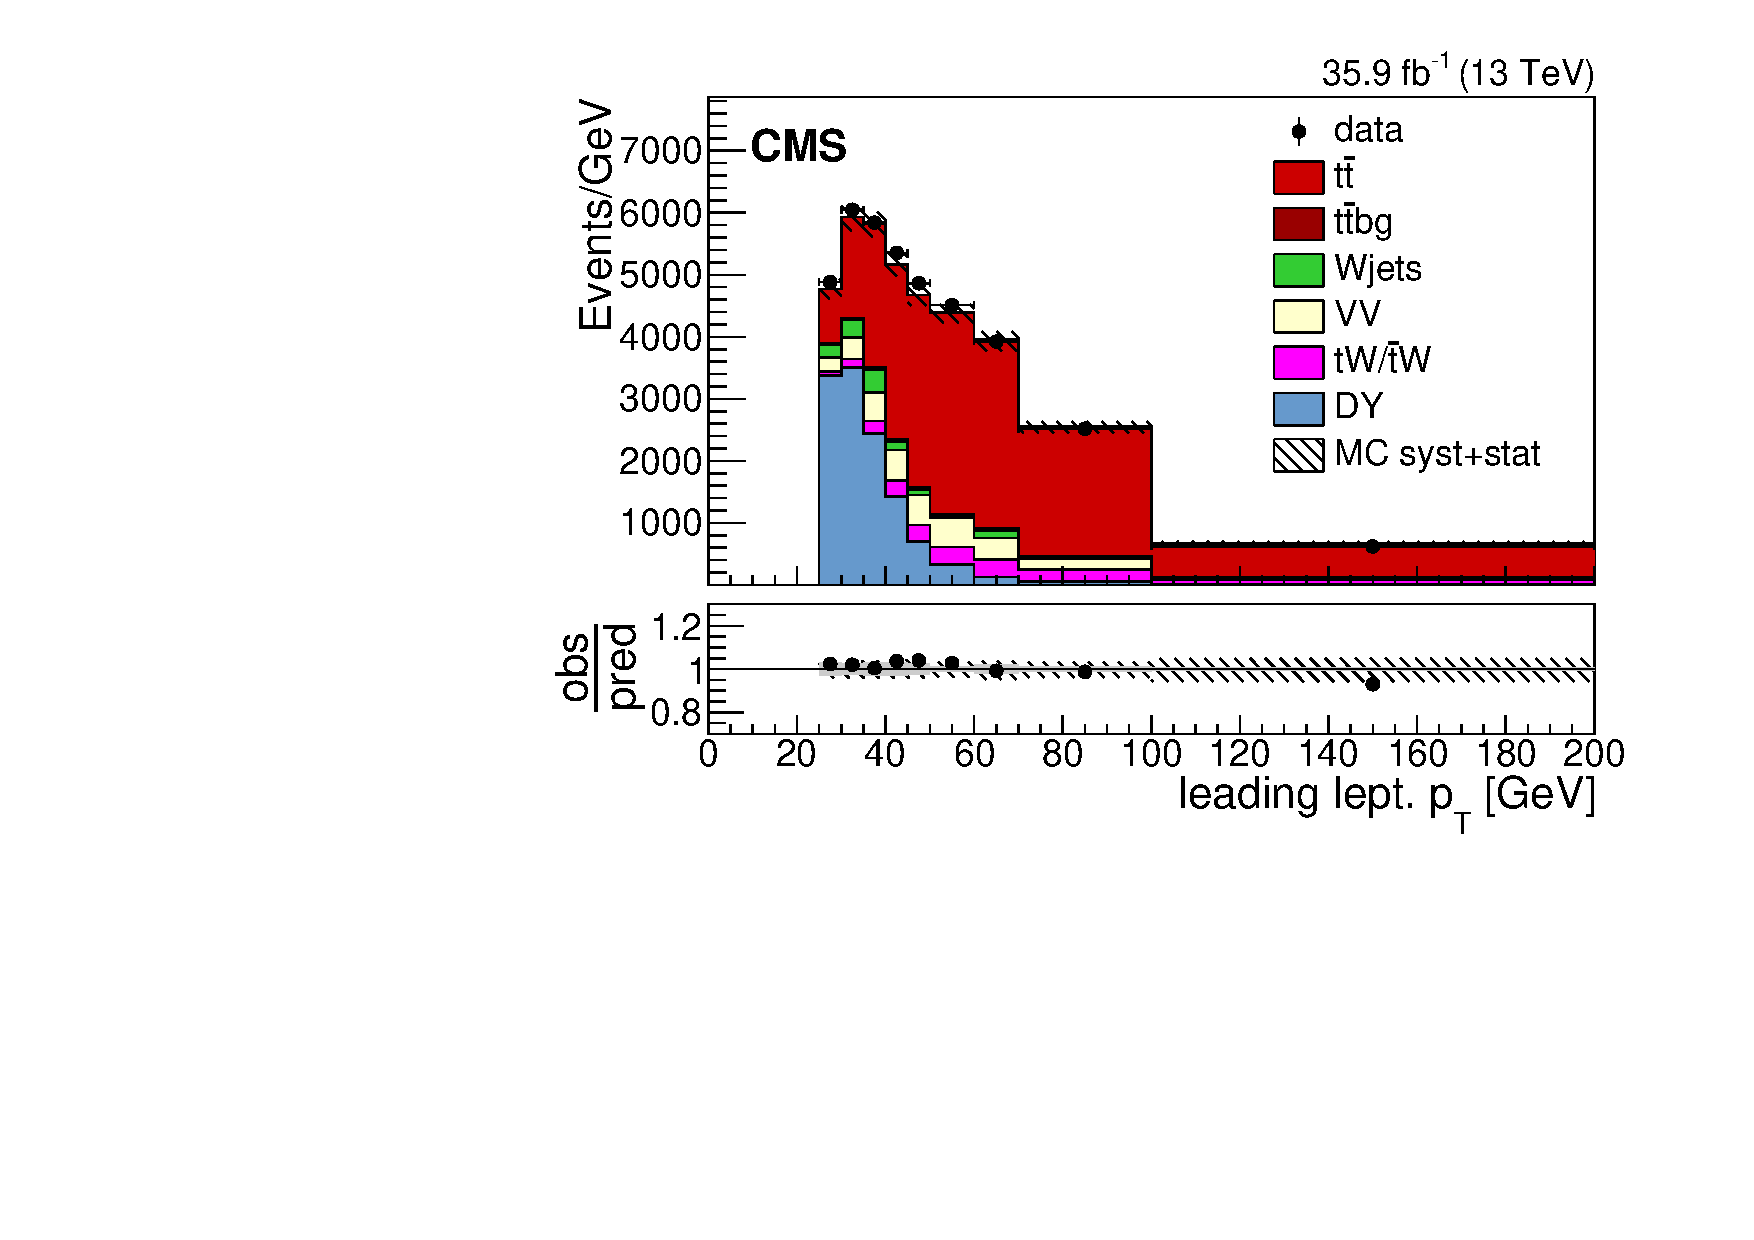
\includegraphics{CrossSection/Figures/ControlPlots/emu_sysnom/lead_lepton_pt_step_8.pdf}}
    \resizebox{0.48 \textwidth}{!}{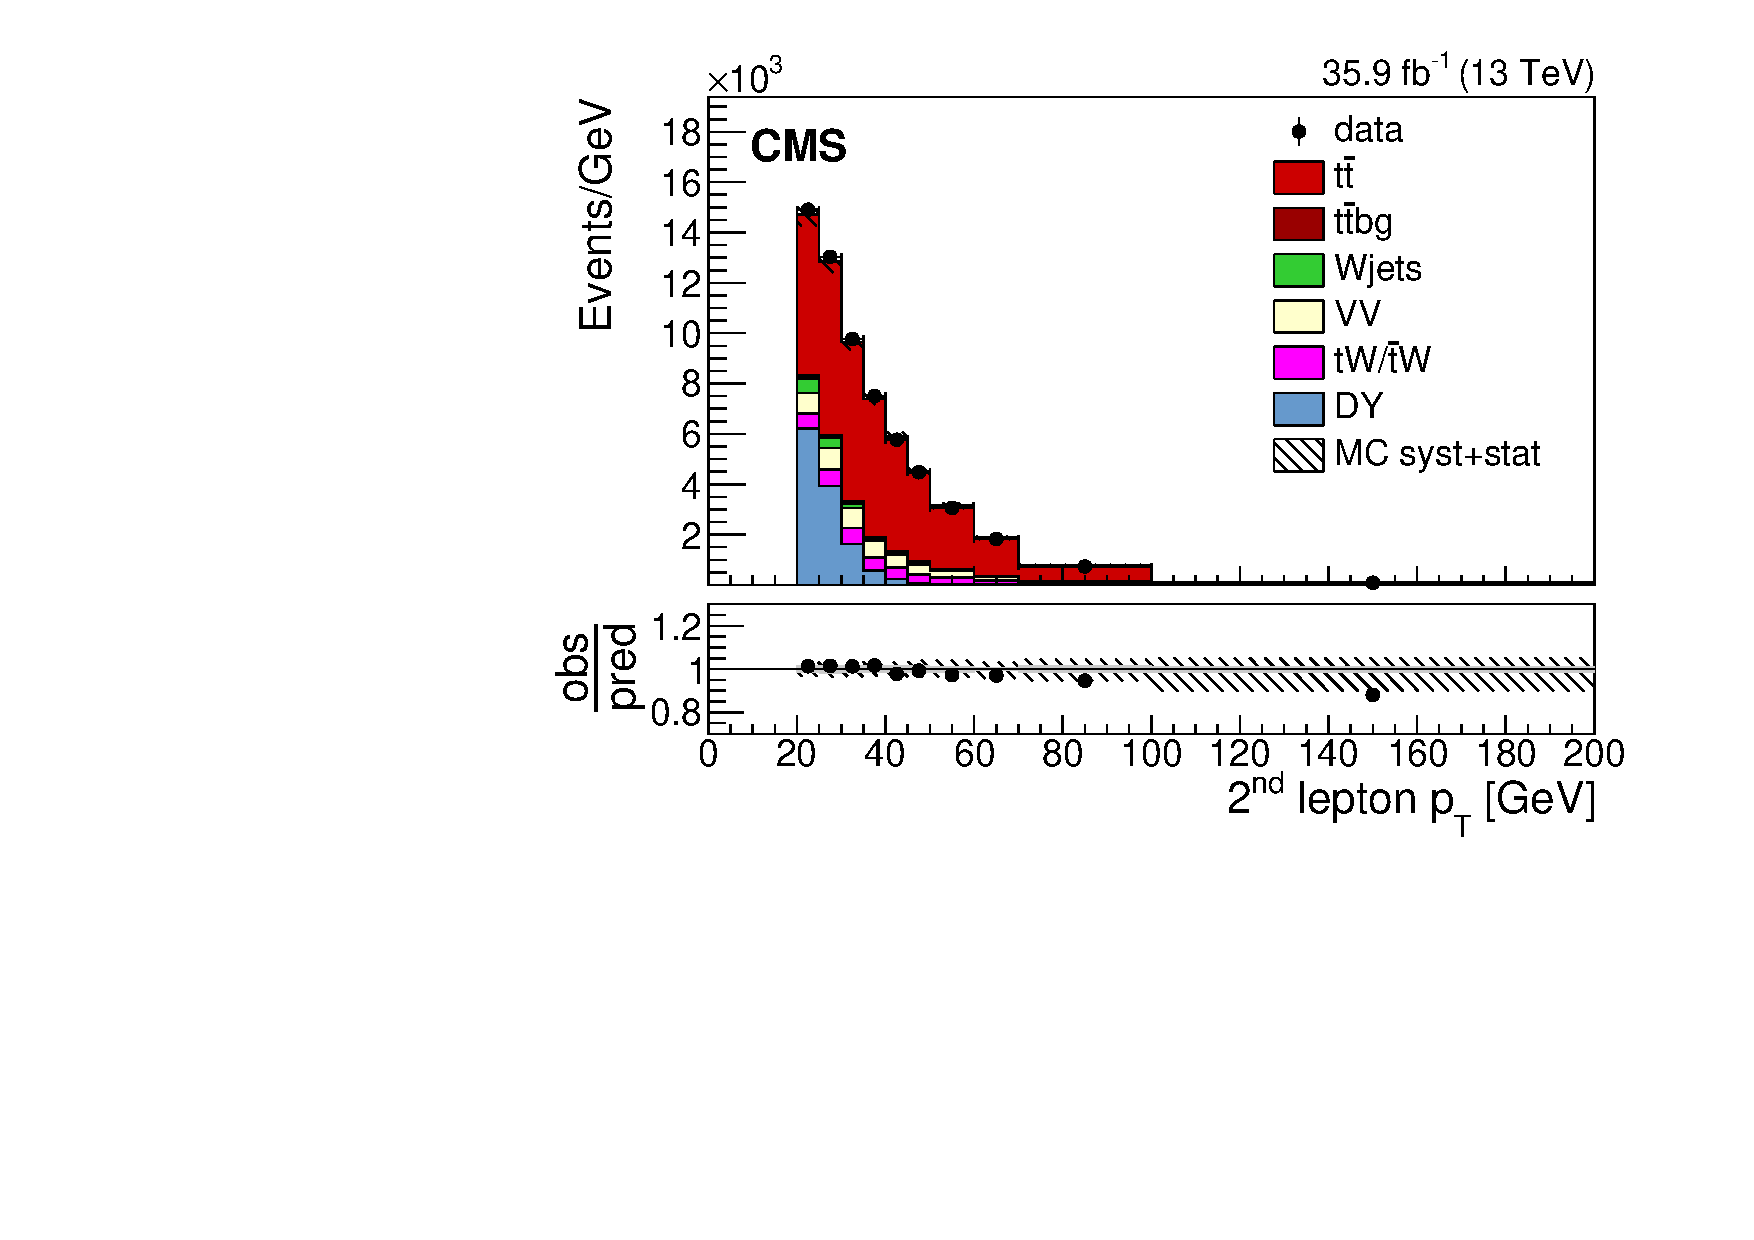
\includegraphics{CrossSection/Figures/ControlPlots/emu_sysnom/seclead_lepton_pt_step_8.pdf}}
        \resizebox{0.48 \textwidth}{!}{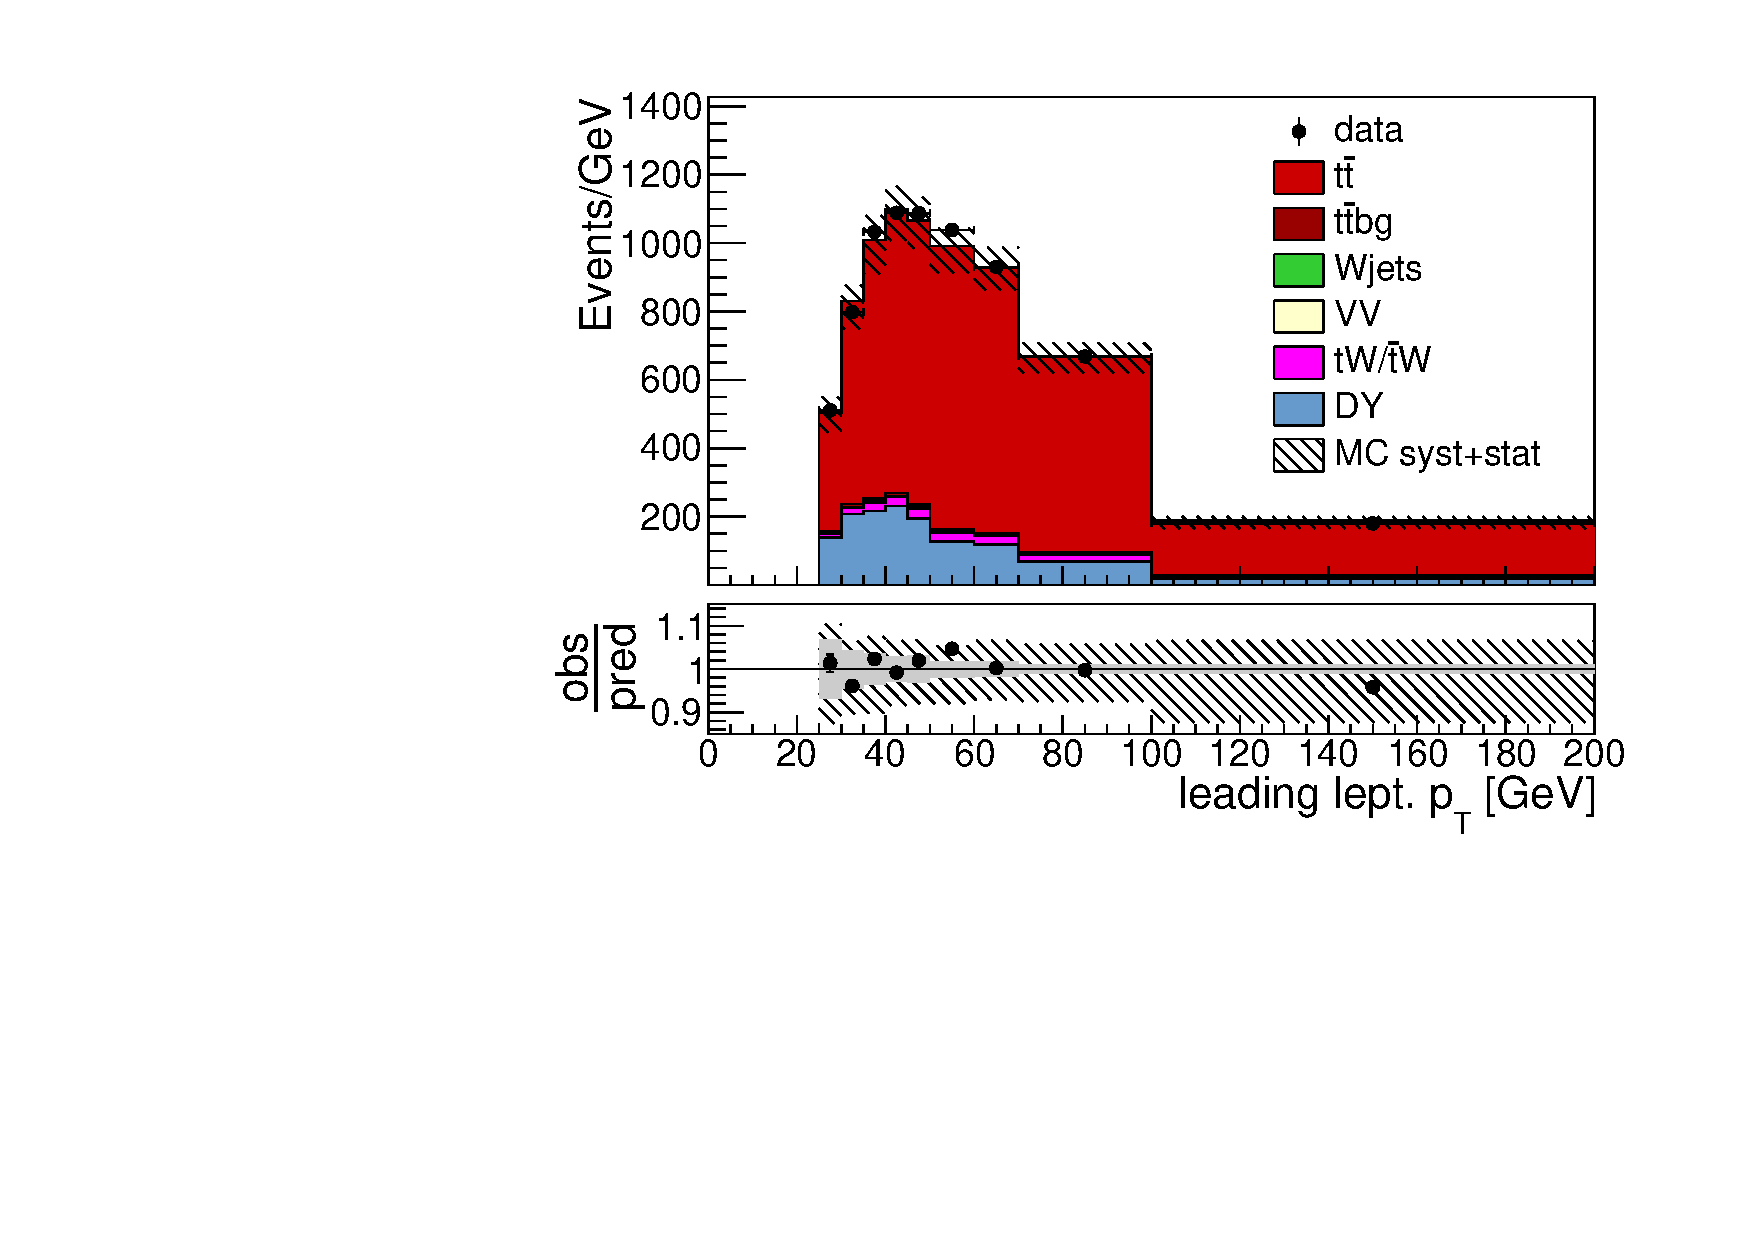
\includegraphics{CrossSection/Figures/ControlPlots/mumu_sysnom/lead_lepton_pt_step_8.pdf}}
    \resizebox{0.48 \textwidth}{!}{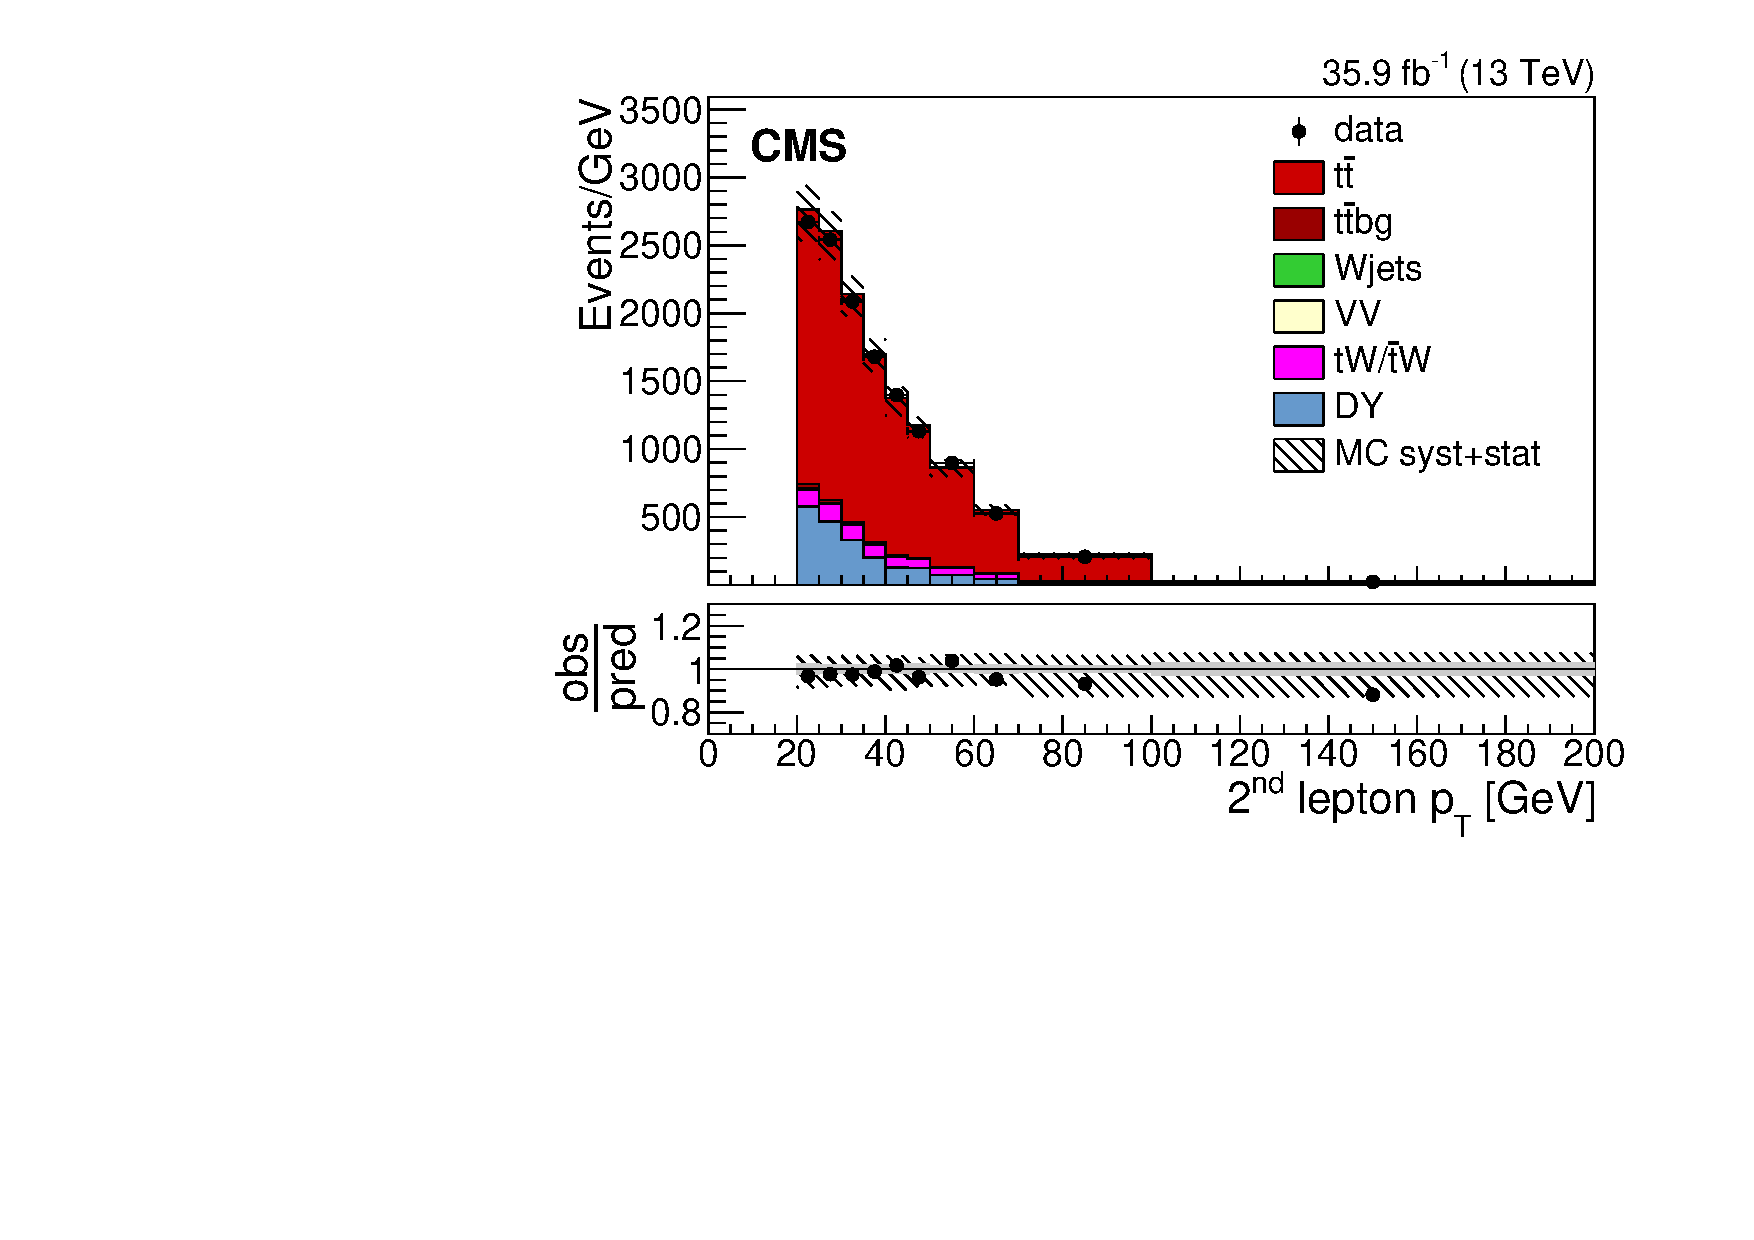
\includegraphics{CrossSection/Figures/ControlPlots/mumu_sysnom/seclead_lepton_pt_step_8.pdf}}
    \resizebox{0.48 \textwidth}{!}{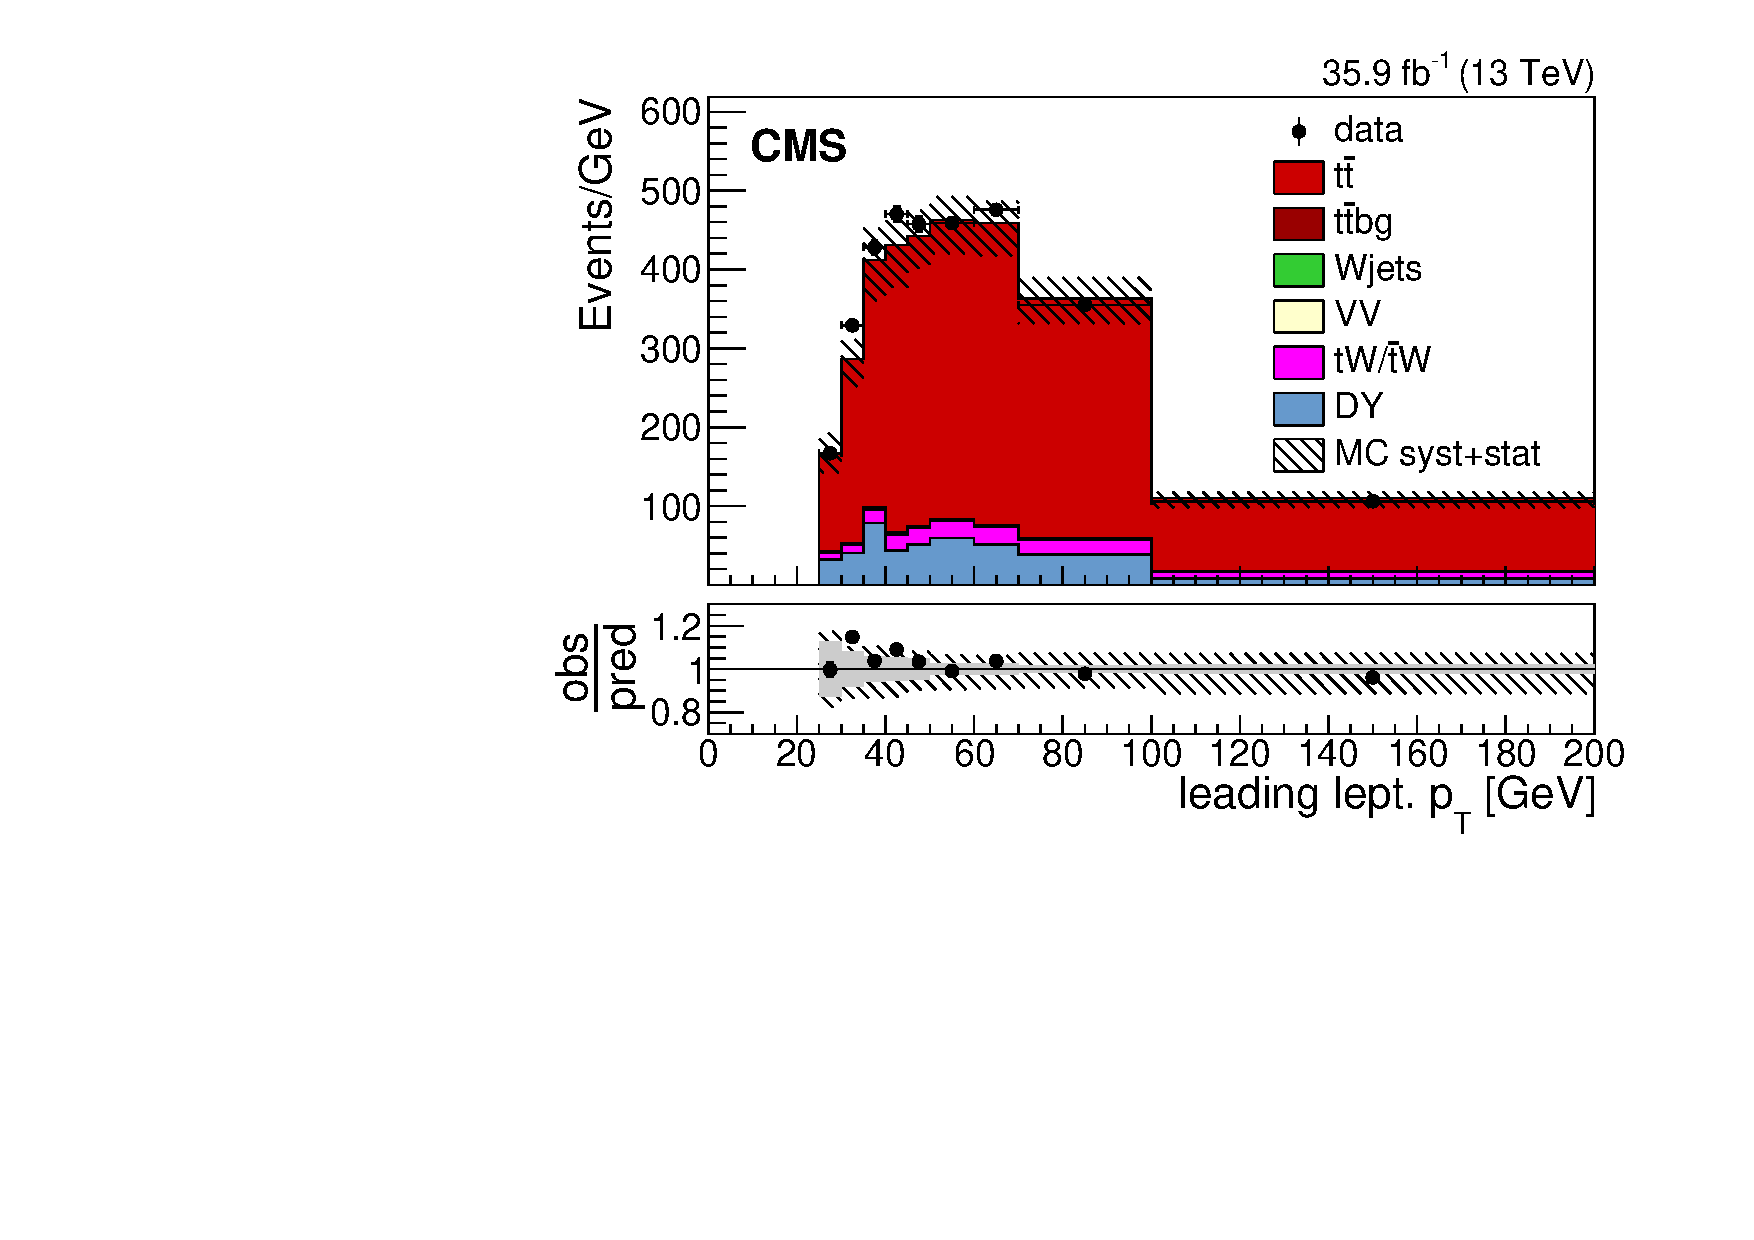
\includegraphics{CrossSection/Figures/ControlPlots/ee_sysnom/lead_lepton_pt_step_8.pdf}}
    \resizebox{0.48 \textwidth}{!}{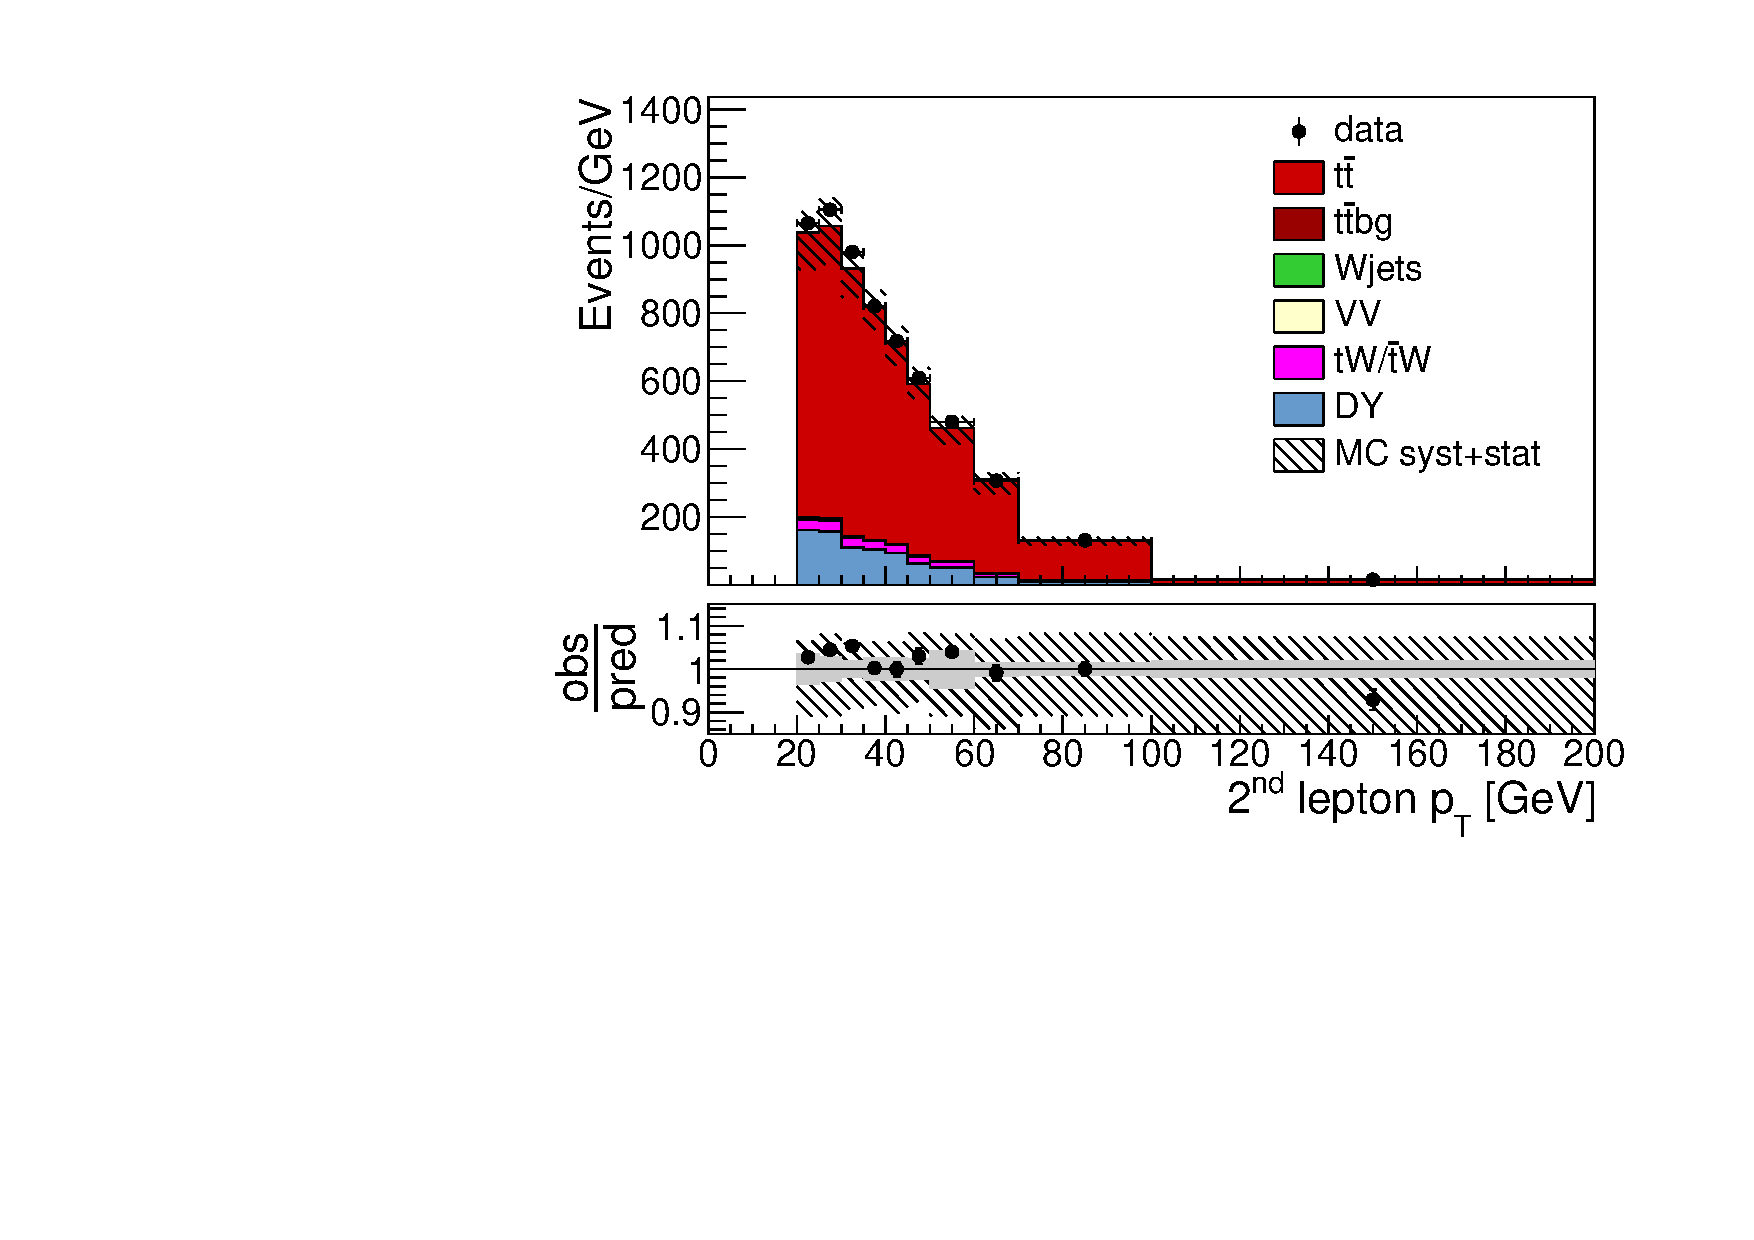
\includegraphics{CrossSection/Figures/ControlPlots/ee_sysnom/seclead_lepton_pt_step_8.pdf}}
      \caption{Transverse momentum of the leading (left) and subleading (right)
        lepton in the \emu (upper row), \mumu (middle row) and \ee (lower row) decay channels.
        The events are shown after the
        event selection.  The hatched
        bands correspond to the total uncertainty on the sum of the
        predicted yields 
        , excluding luminosity and background
        normalization uncertainties. 
        The ratios of data to the sum of the predicted yields are
        shown at the bottom panel of each figure. The solid gray band
        represents the contribution of the statistical uncertainty.}  
       \label{fig:xsec_pt_ctrplots}
  \end{center}
\end{figure}

The $\eta$ distribution for the leading and subleading lepton for all three decay channels is shown in Figure~\ref{fig:xsec_eta_ctrplots}.
For electrons (\emu and \ee channel) the $\eta$ distribution shows a gap around $|\eta| \approx 1.5$. This reduction in the number of events is caused by an instrumentation gap in the ECAL (see Section~\ref{sec:xsec_sel}).
Otherwise, the $\eta$ distribution is smooth as seen for the \mumu channel.
The simulation generally agrees with the data within uncertainties. The systematic uncertainties are generally higher for larger $\eta$ values, as uncertainties on the lepton reconstruction
tend to increase if the lepton is detected in the endcaps of the detector.


\begin{figure}[htbp!]
  \begin{center}
    \resizebox{0.48 \textwidth}{!}{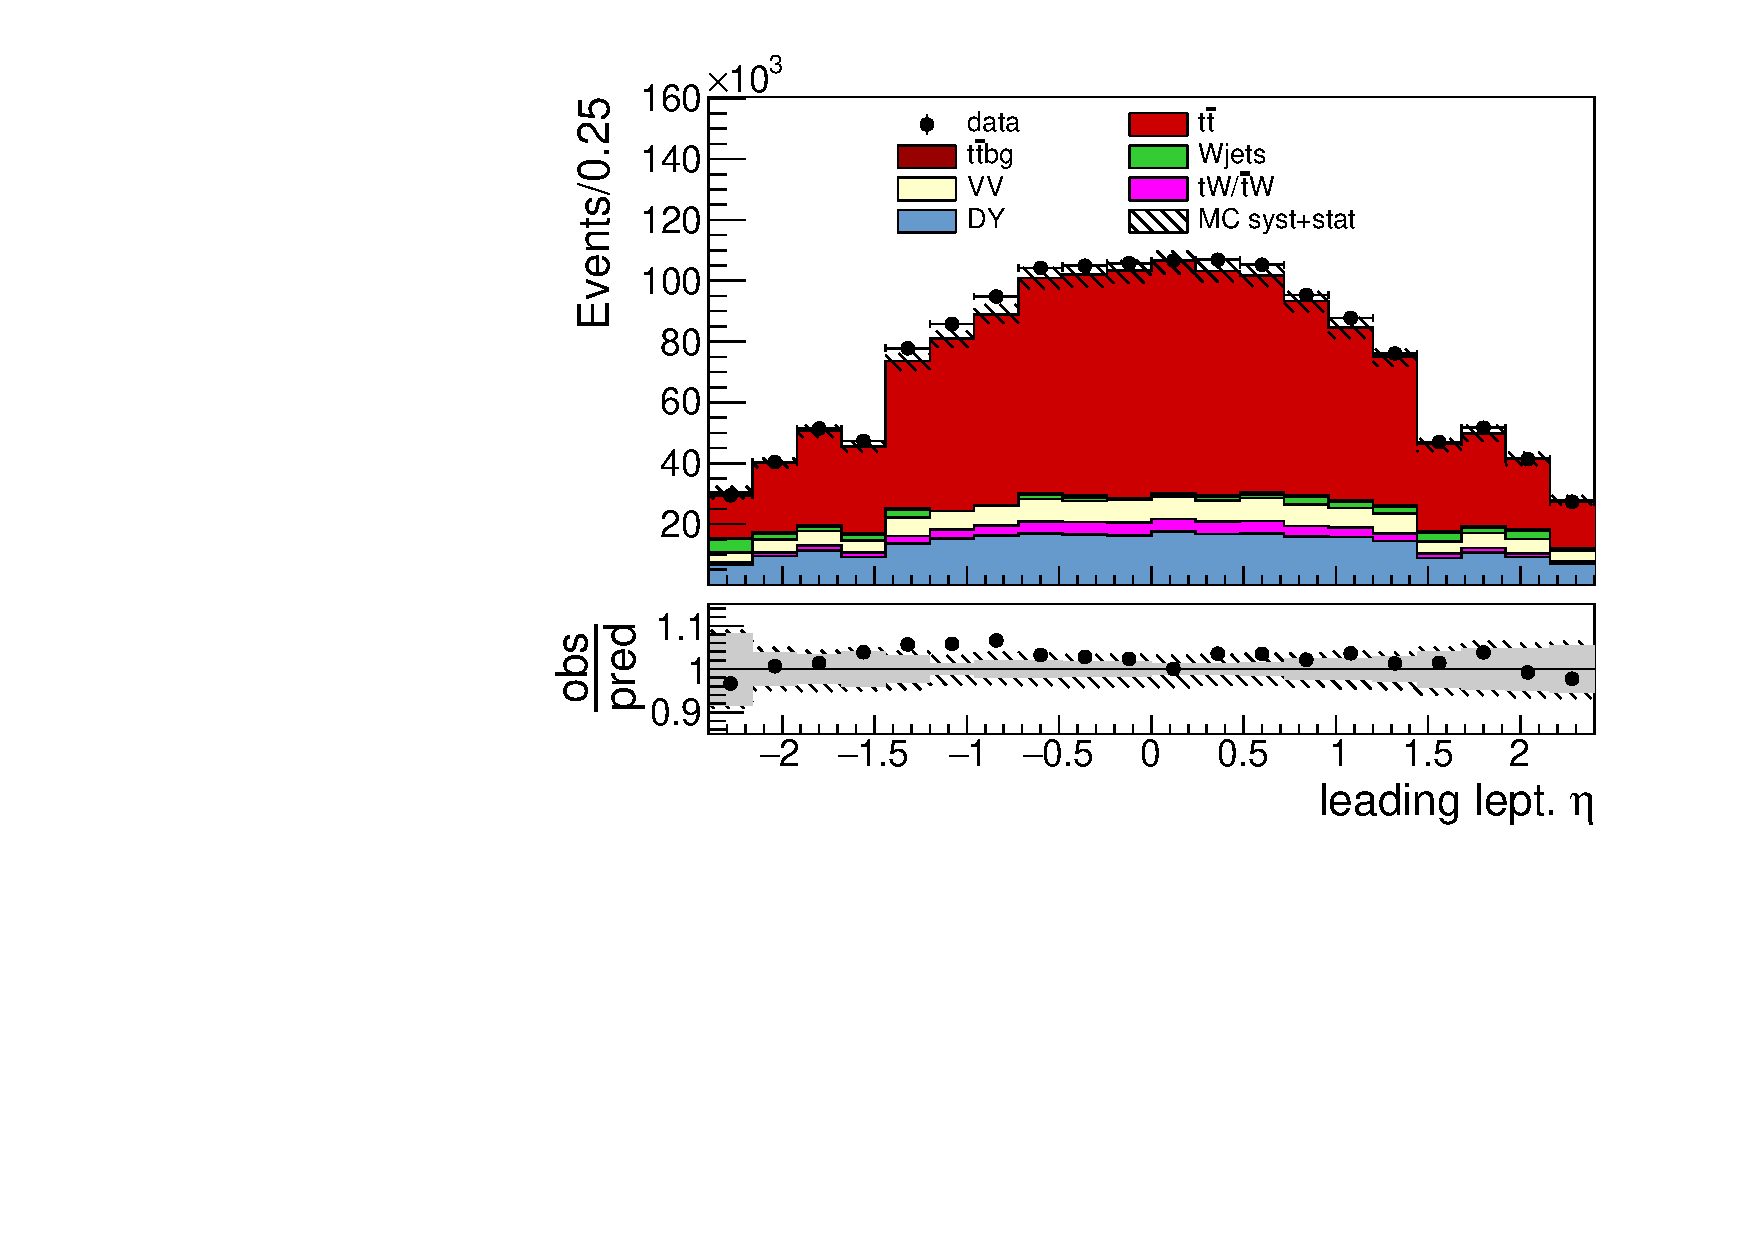
\includegraphics{CrossSection/Figures/ControlPlots/emu_sysnom/lead_lepton_eta_step_8.pdf}}
    \resizebox{0.48 \textwidth}{!}{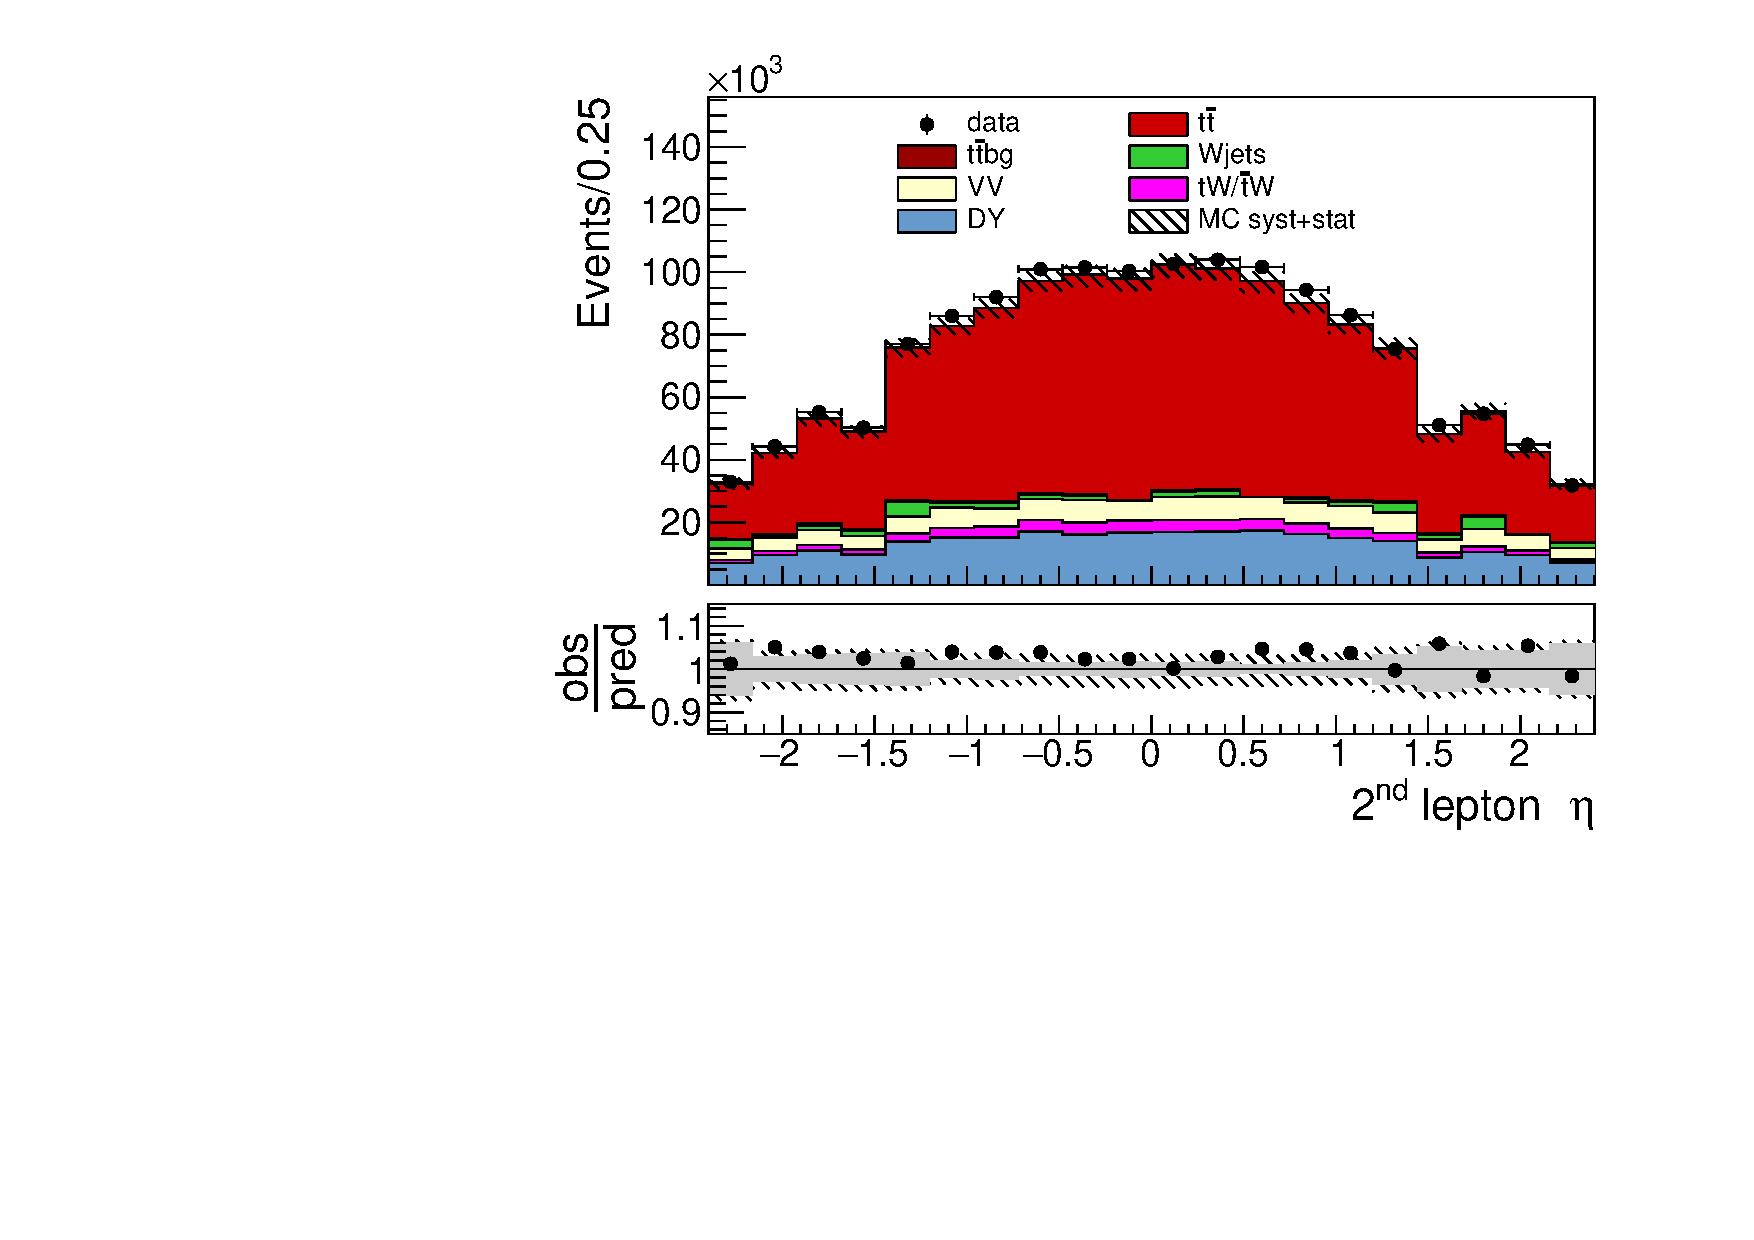
\includegraphics{CrossSection/Figures/ControlPlots/emu_sysnom/seclead_lepton_eta_step_8.pdf}}
        \resizebox{0.48 \textwidth}{!}{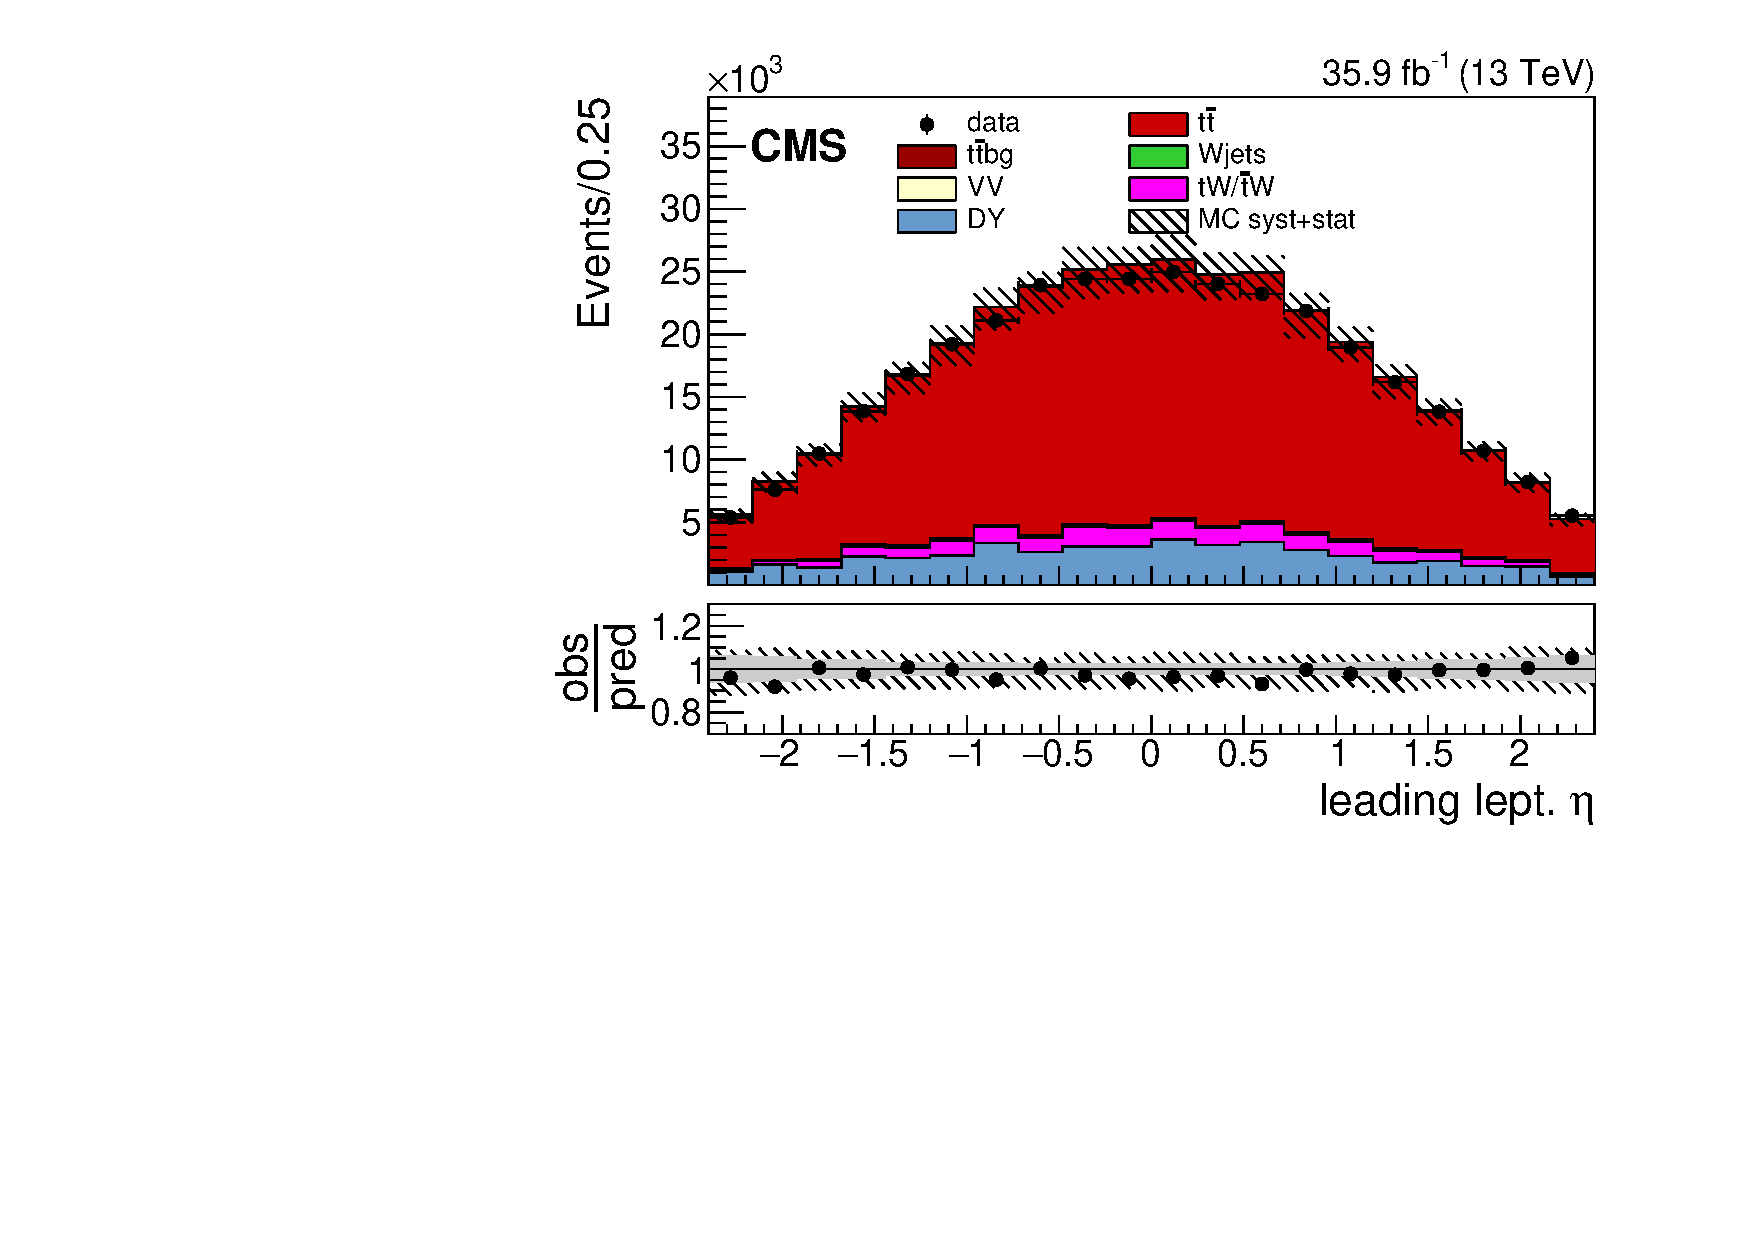
\includegraphics{CrossSection/Figures/ControlPlots/mumu_sysnom/lead_lepton_eta_step_8.pdf}}
    \resizebox{0.48 \textwidth}{!}{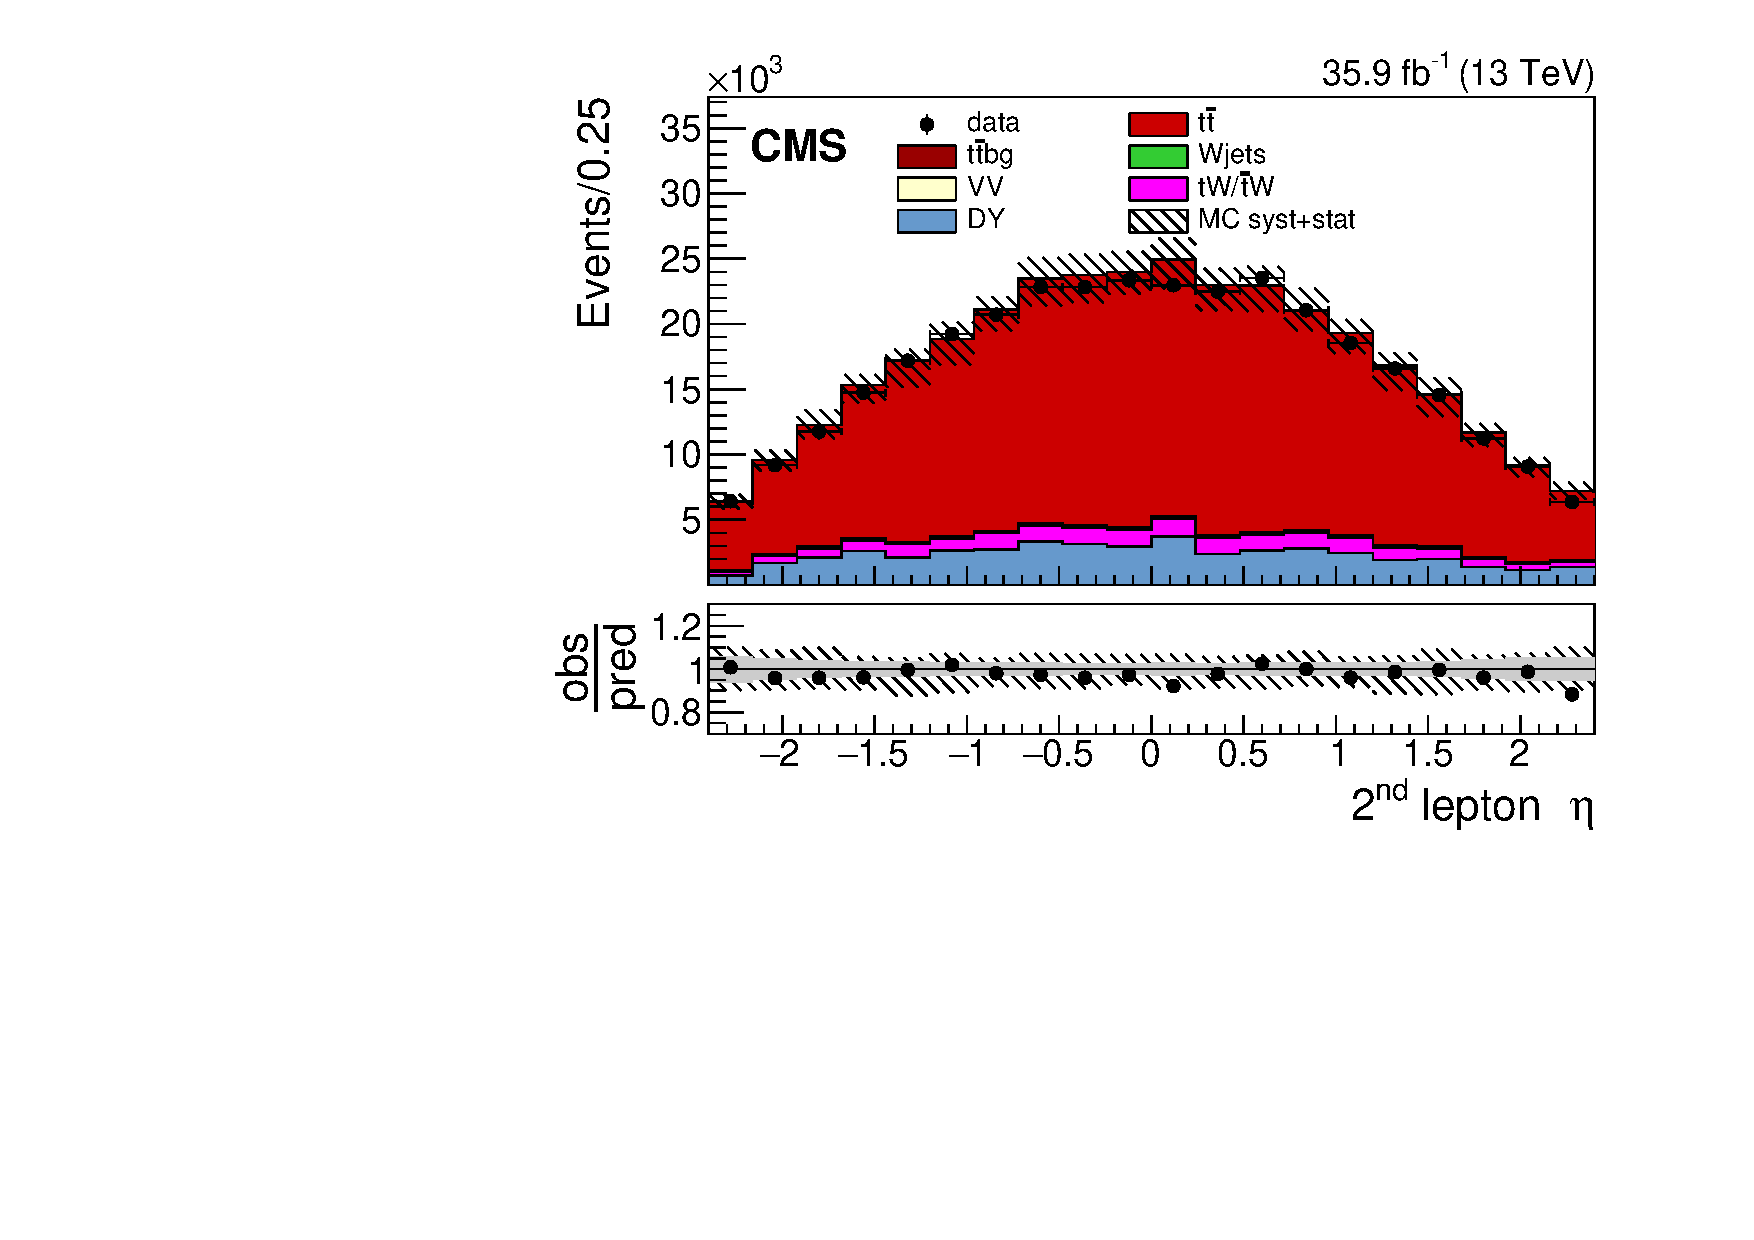
\includegraphics{CrossSection/Figures/ControlPlots/mumu_sysnom/seclead_lepton_eta_step_8.pdf}}
    \resizebox{0.48 \textwidth}{!}{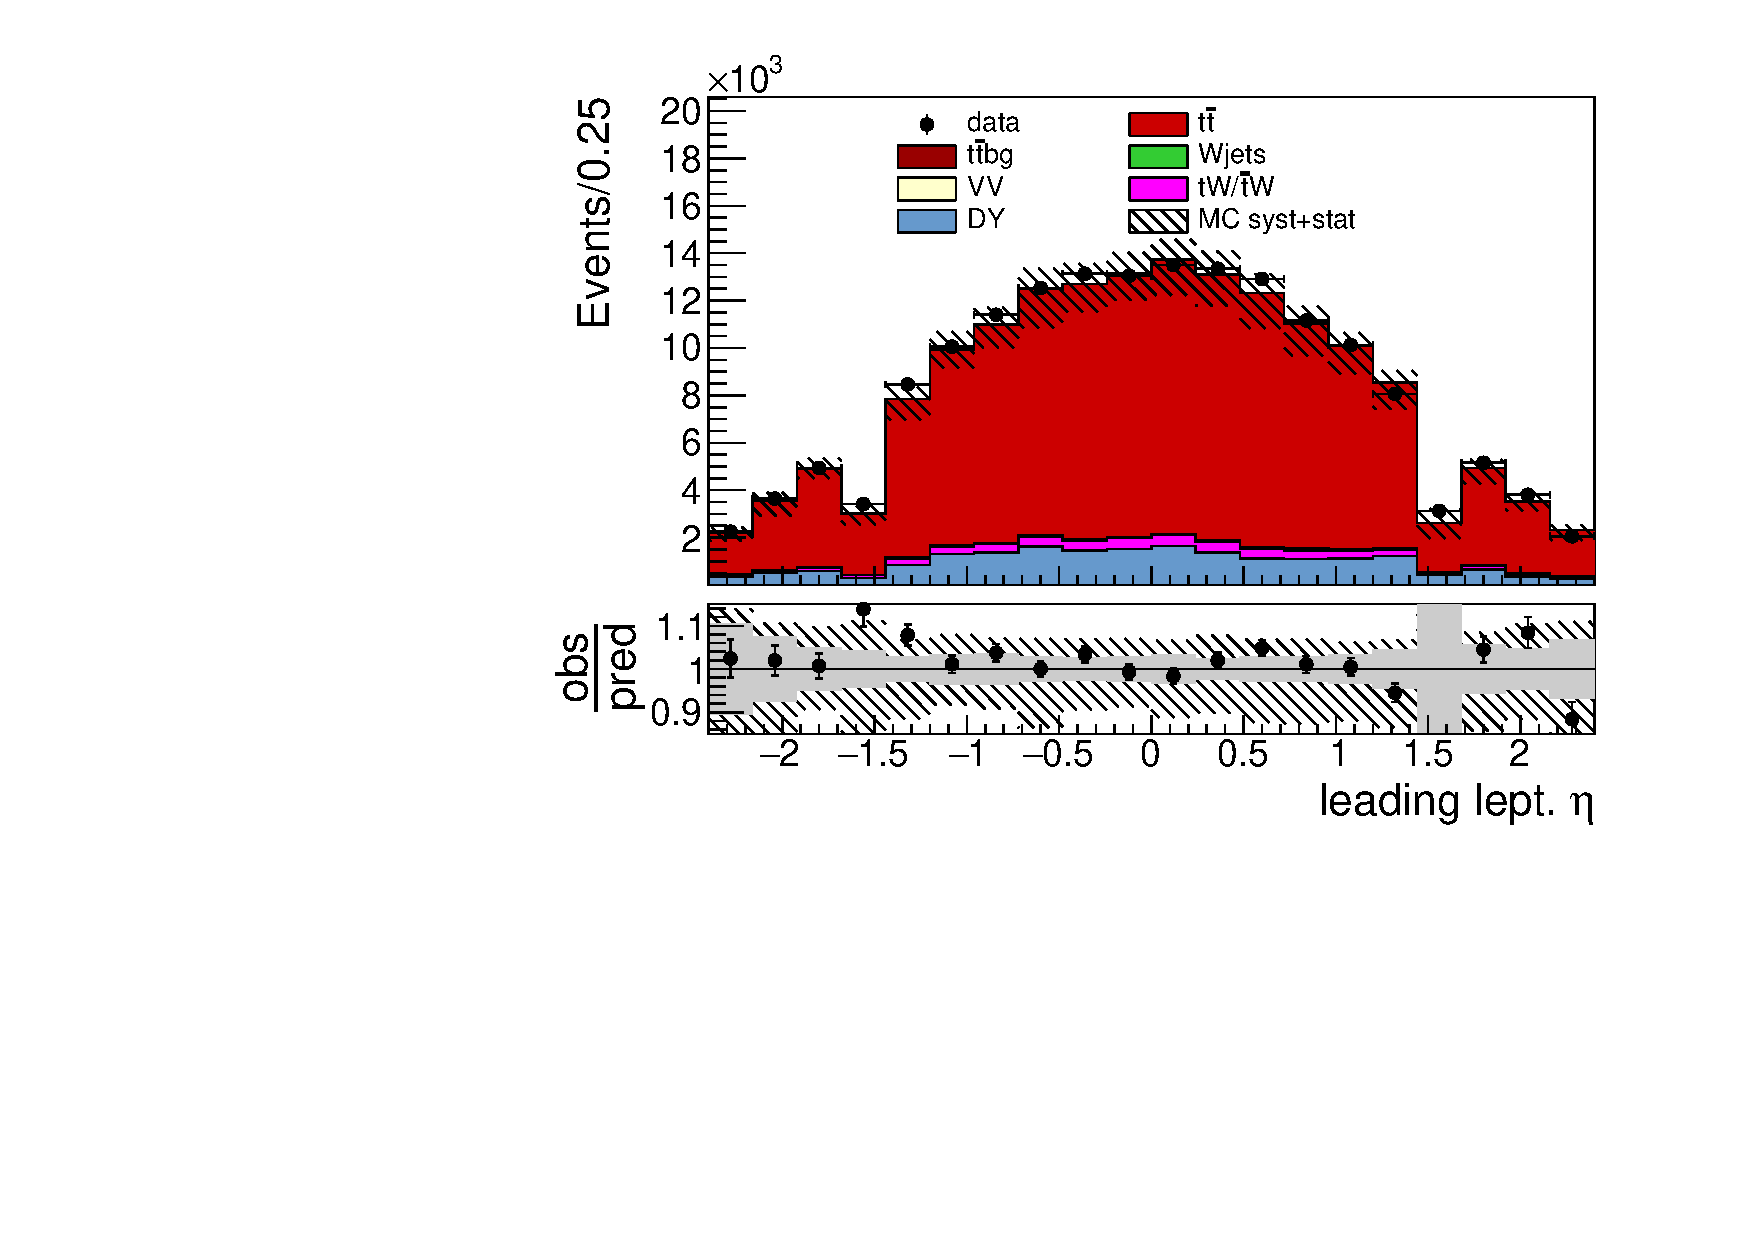
\includegraphics{CrossSection/Figures/ControlPlots/ee_sysnom/lead_lepton_eta_step_8.pdf}}
    \resizebox{0.48 \textwidth}{!}{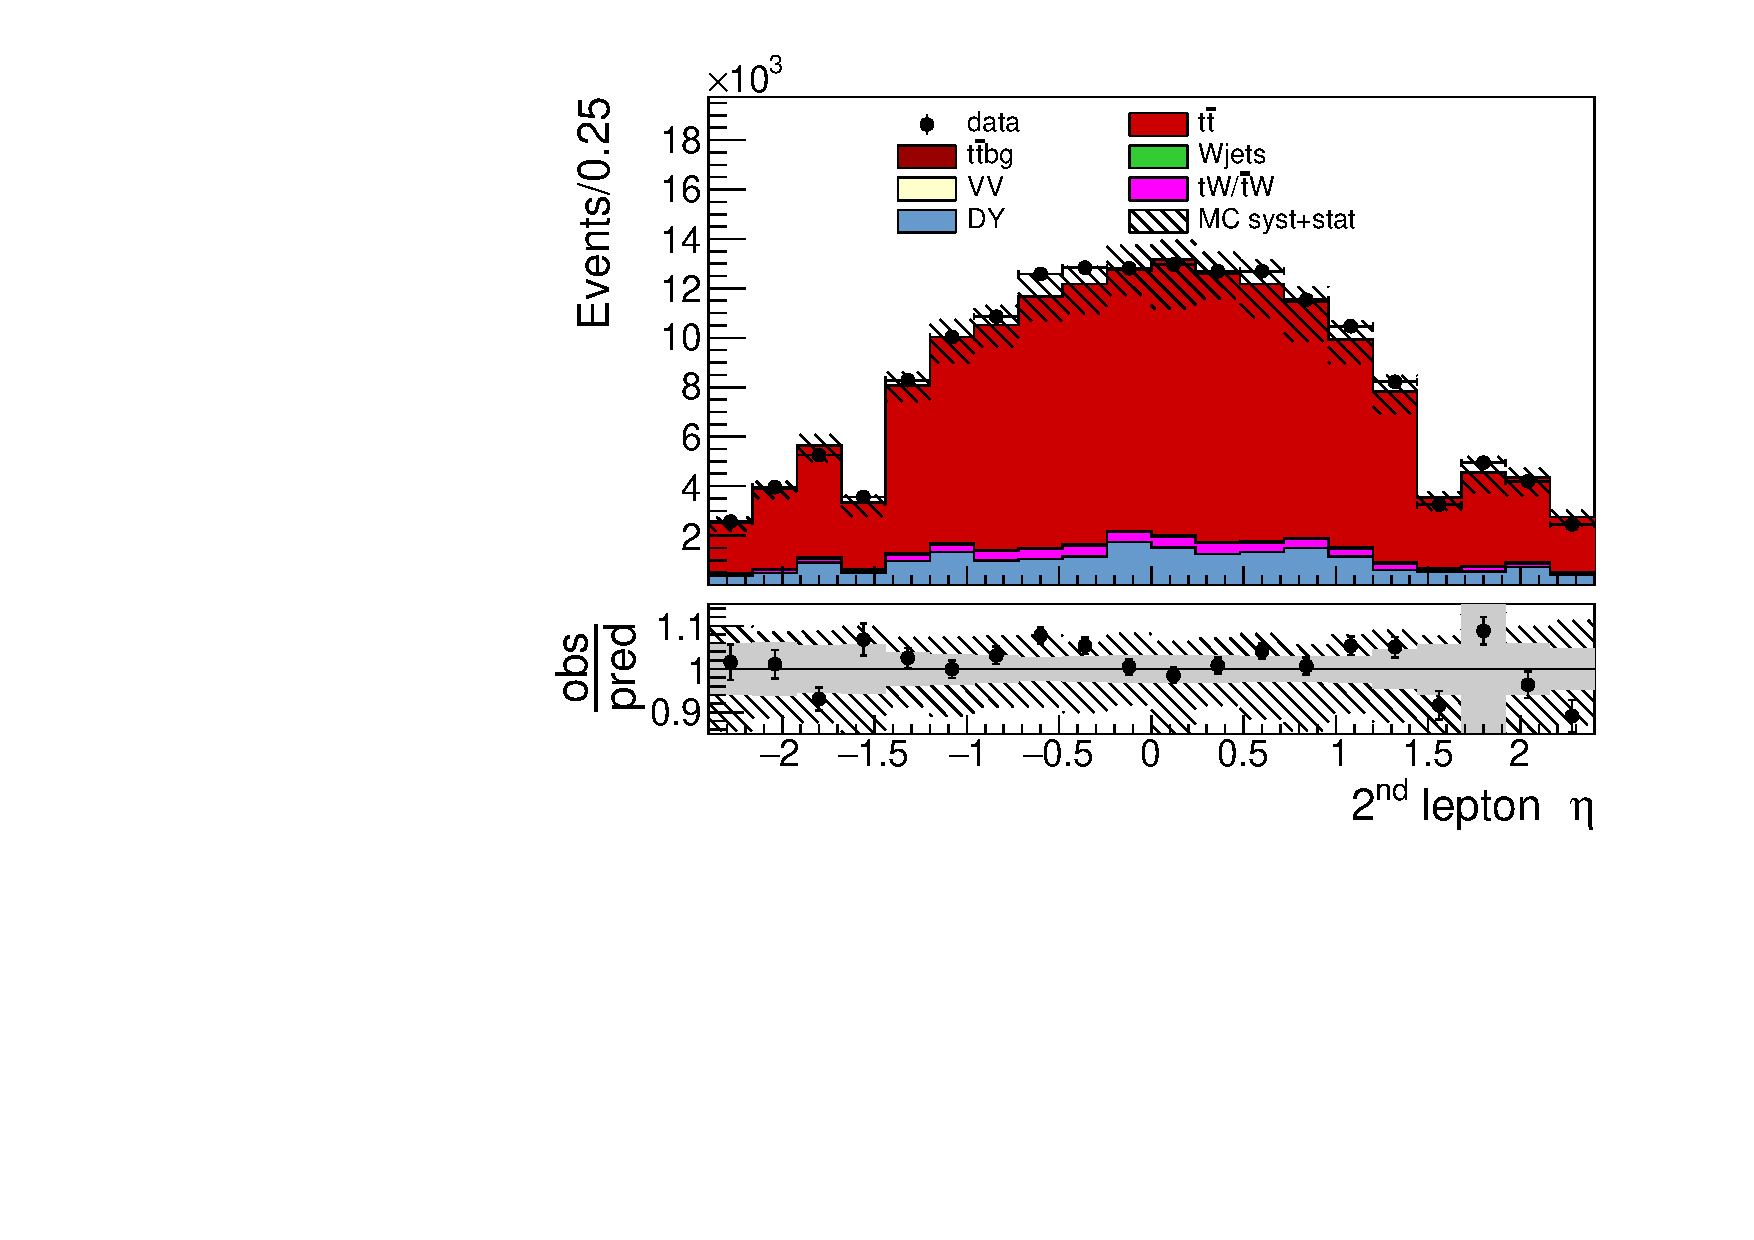
\includegraphics{CrossSection/Figures/ControlPlots/ee_sysnom/seclead_lepton_eta_step_8.pdf}}
      \caption{Pseudo rapidity for the leading (left) and subleading (right)
        lepton in the \emu (upper row), \mumu (middle row) and \ee (lower row) decay channels.
        The events are shown after the
        event selection.  The hatched
        bands correspond to the total uncertainty on the sum of the
        predicted yields, 
        excluding luminosity and background
        normalization uncertainties. 
        The ratios of data to the sum of the predicted yields are
        shown in the bottom panel of each figure. The solid gray band
        represents the contribution of the statistical uncertainty.}  
       \label{fig:xsec_eta_ctrplots}
  \end{center}
\end{figure}



The number of jets for all three channels is shown in Figure~\ref{fig:xsec_jets_ctrplots}.
The largest number of \ttbar events is found in the bin with exactly two jets. 
Events with zero jets are rejected for the \ee and \mumu channel, but the \emu channel shows that the signal
contribution in that region of phase space is comparatively small.
As seen in all channels, \ttbar signal events tend to contain more jets compared to background events, as two jets come from the top quark decays and gluons can be radiated from both the initial state and the final state. 
In Drell-Yan events with two leptons, radiation of additional gluons is only possible for the initial state quarks.

The simulation and the data do not agree for a high number of jets in the \emu and \mumu channels.
In the specific simulation used here (see Section~\ref{sec:SimReco_Sim}) up to three jets are simulated in the hard process, while any other jets are produced in the parton shower.
The more extreme ranges of the phase space, such as events with more than five additional jets, are not well modeled.
This is a well-known issue in the simulation of \ttbar events and as shown in the figures it is well covered by the systematic uncertainties. Especially the systematic variations for the parton shower parameters chosen for the simulation
(see Section~\ref{sec:theo_uncert}) contribute in this region of phase space.
In the \ee channel the statistical uncertainty on both the data and the simulation is too large to draw decisive conclusions.

\begin{figure}[htbp!]
  \begin{center}
    \resizebox{0.48 \textwidth}{!}{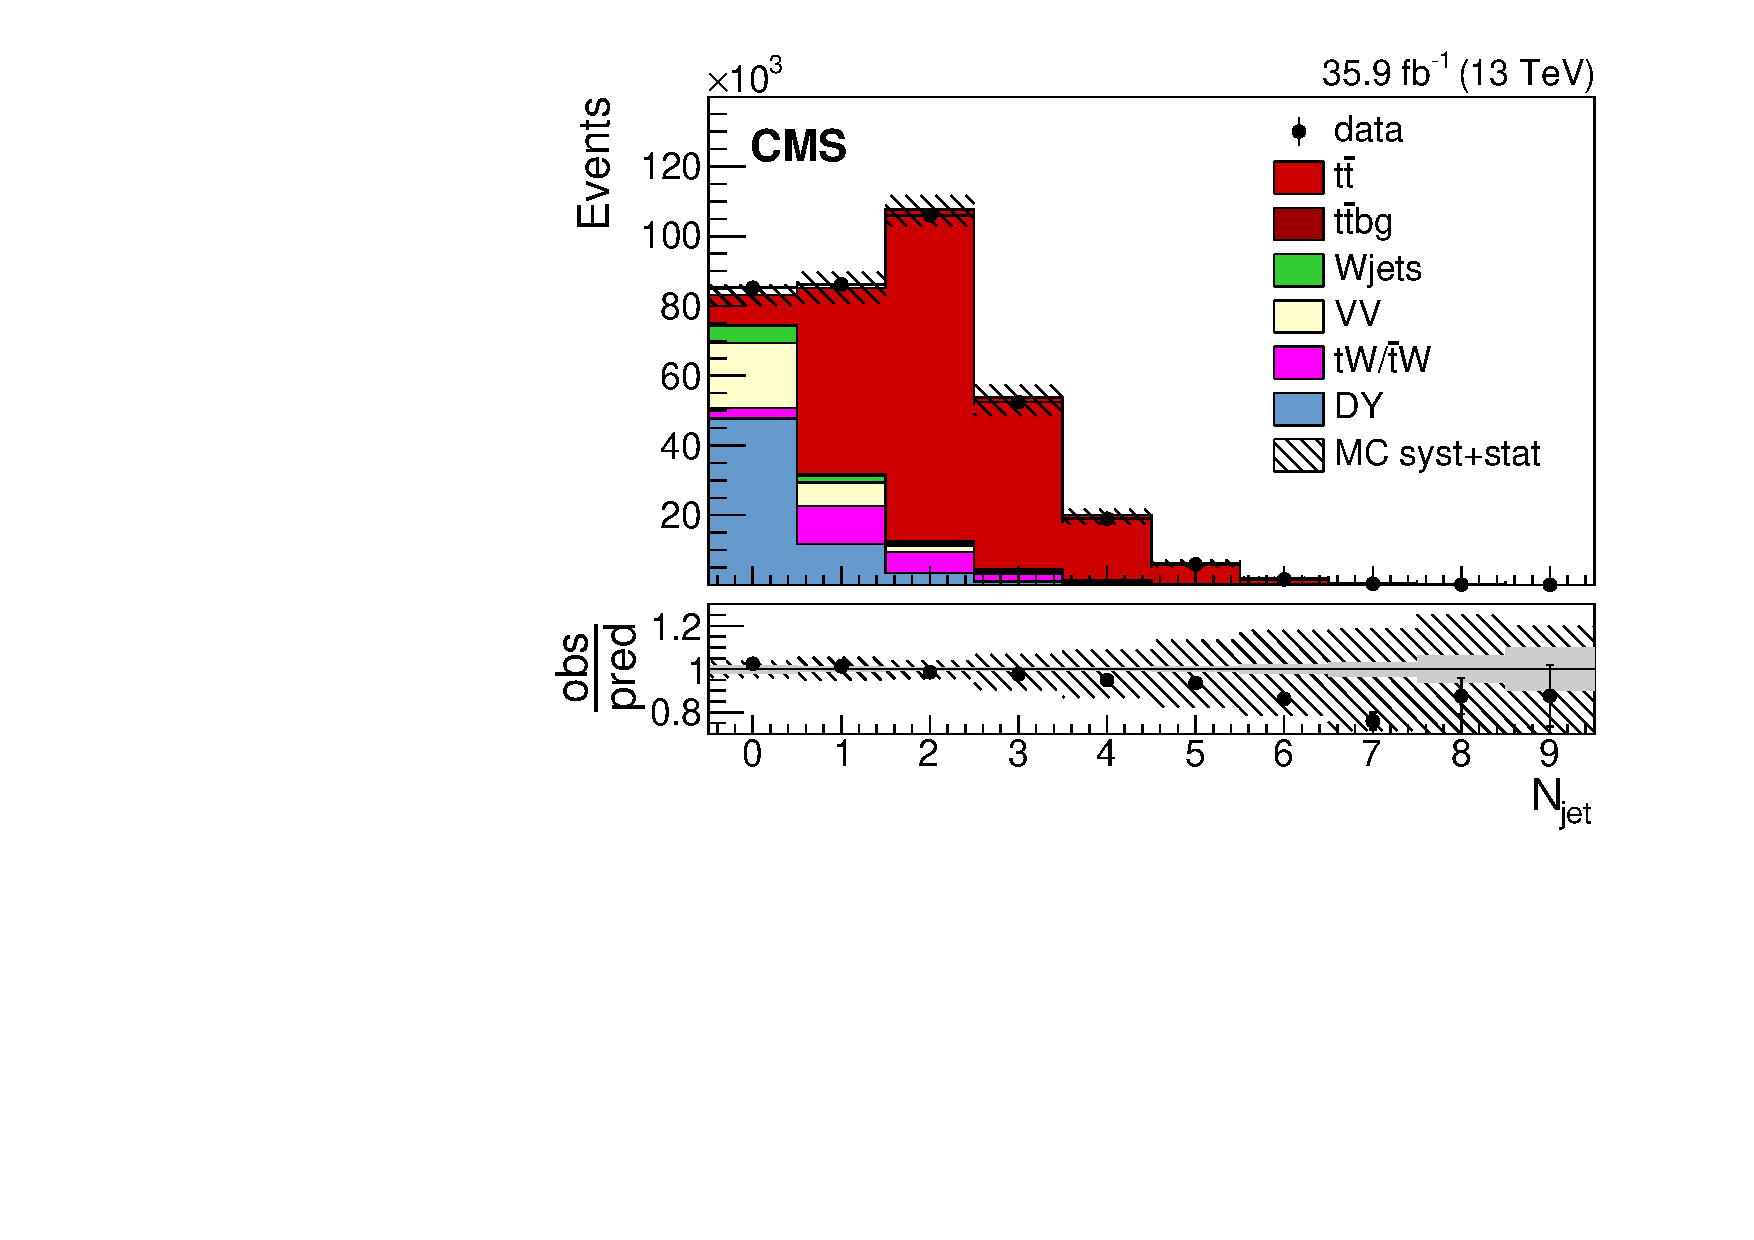
\includegraphics{CrossSection/Figures/ControlPlots/emu_sysnom/selected_jets_multi_step_8.pdf}}
    \resizebox{0.48 \textwidth}{!}{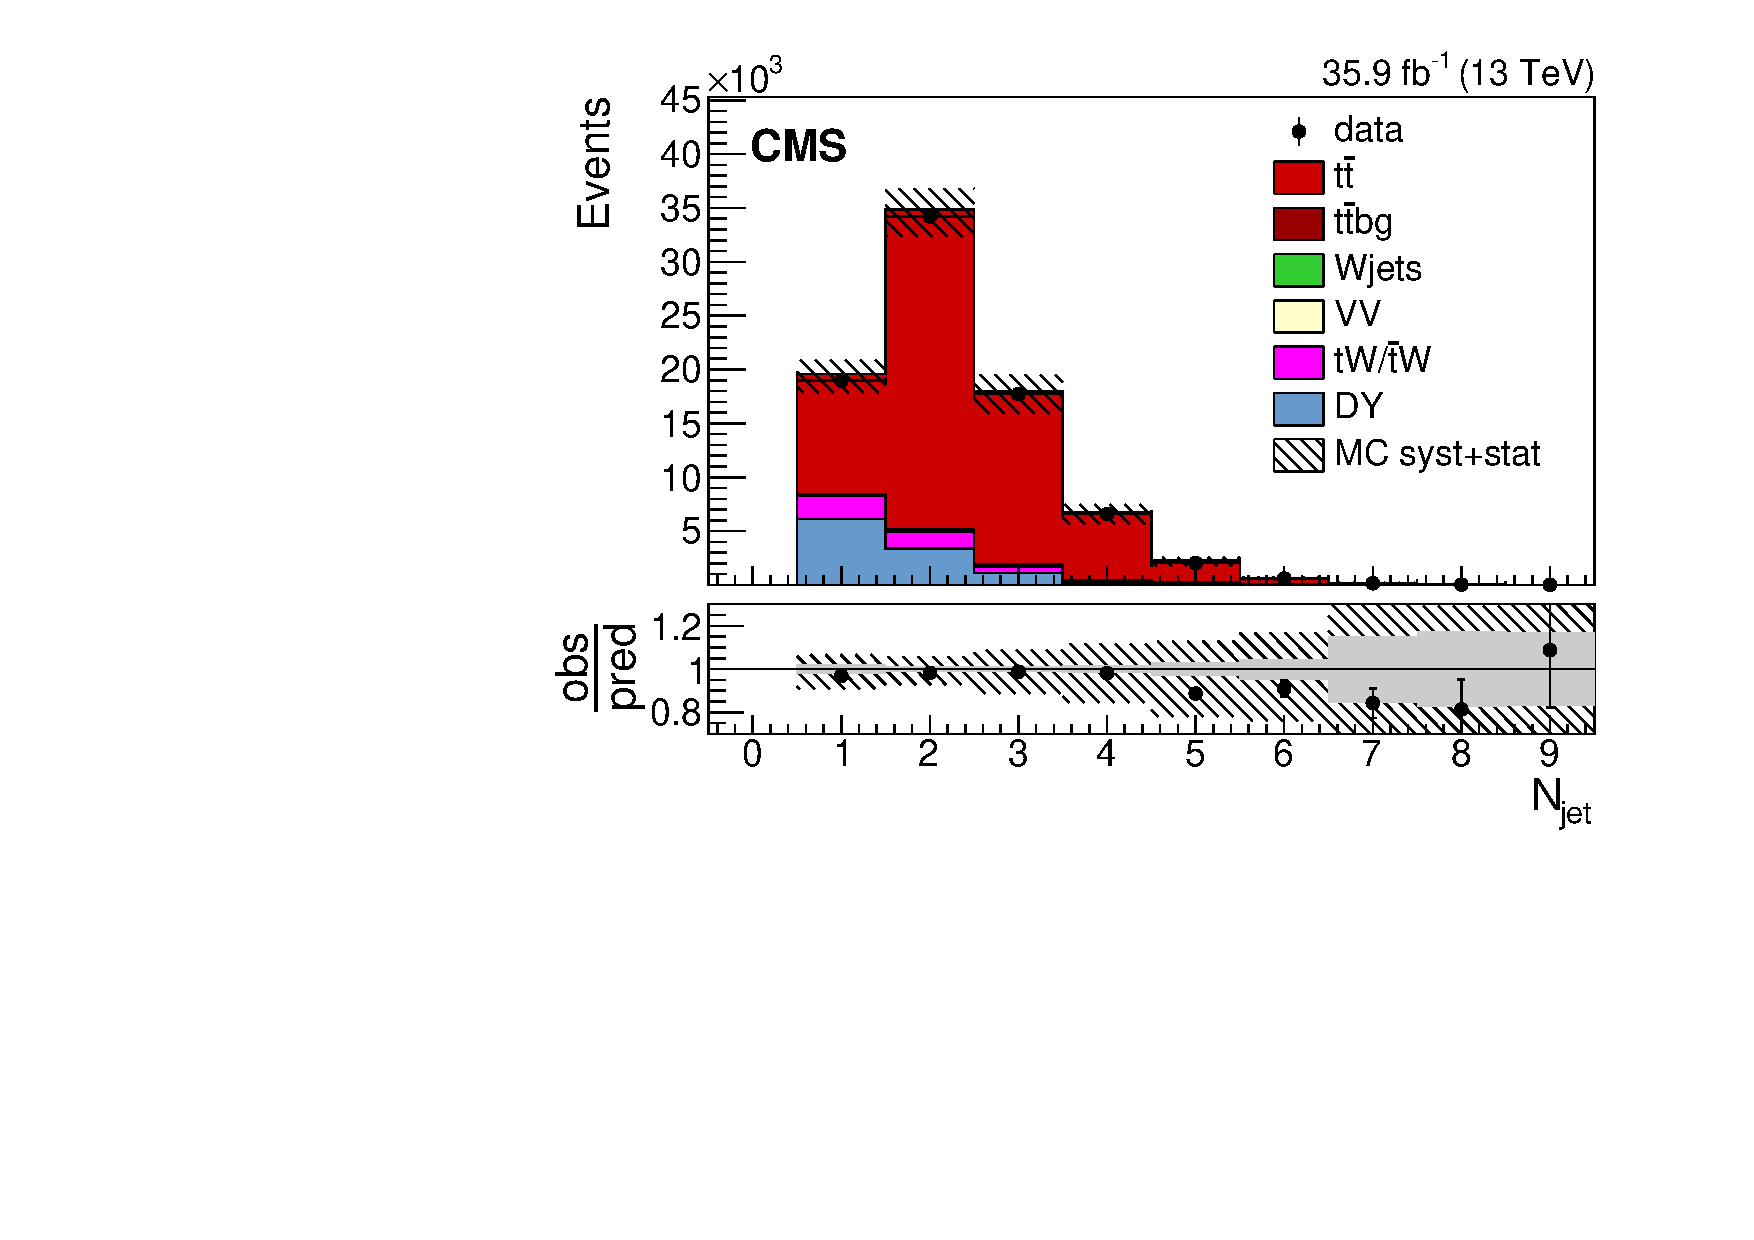
\includegraphics{CrossSection/Figures/ControlPlots/mumu_sysnom/selected_jets_multi_step_8.pdf}}
    \resizebox{0.48 \textwidth}{!}{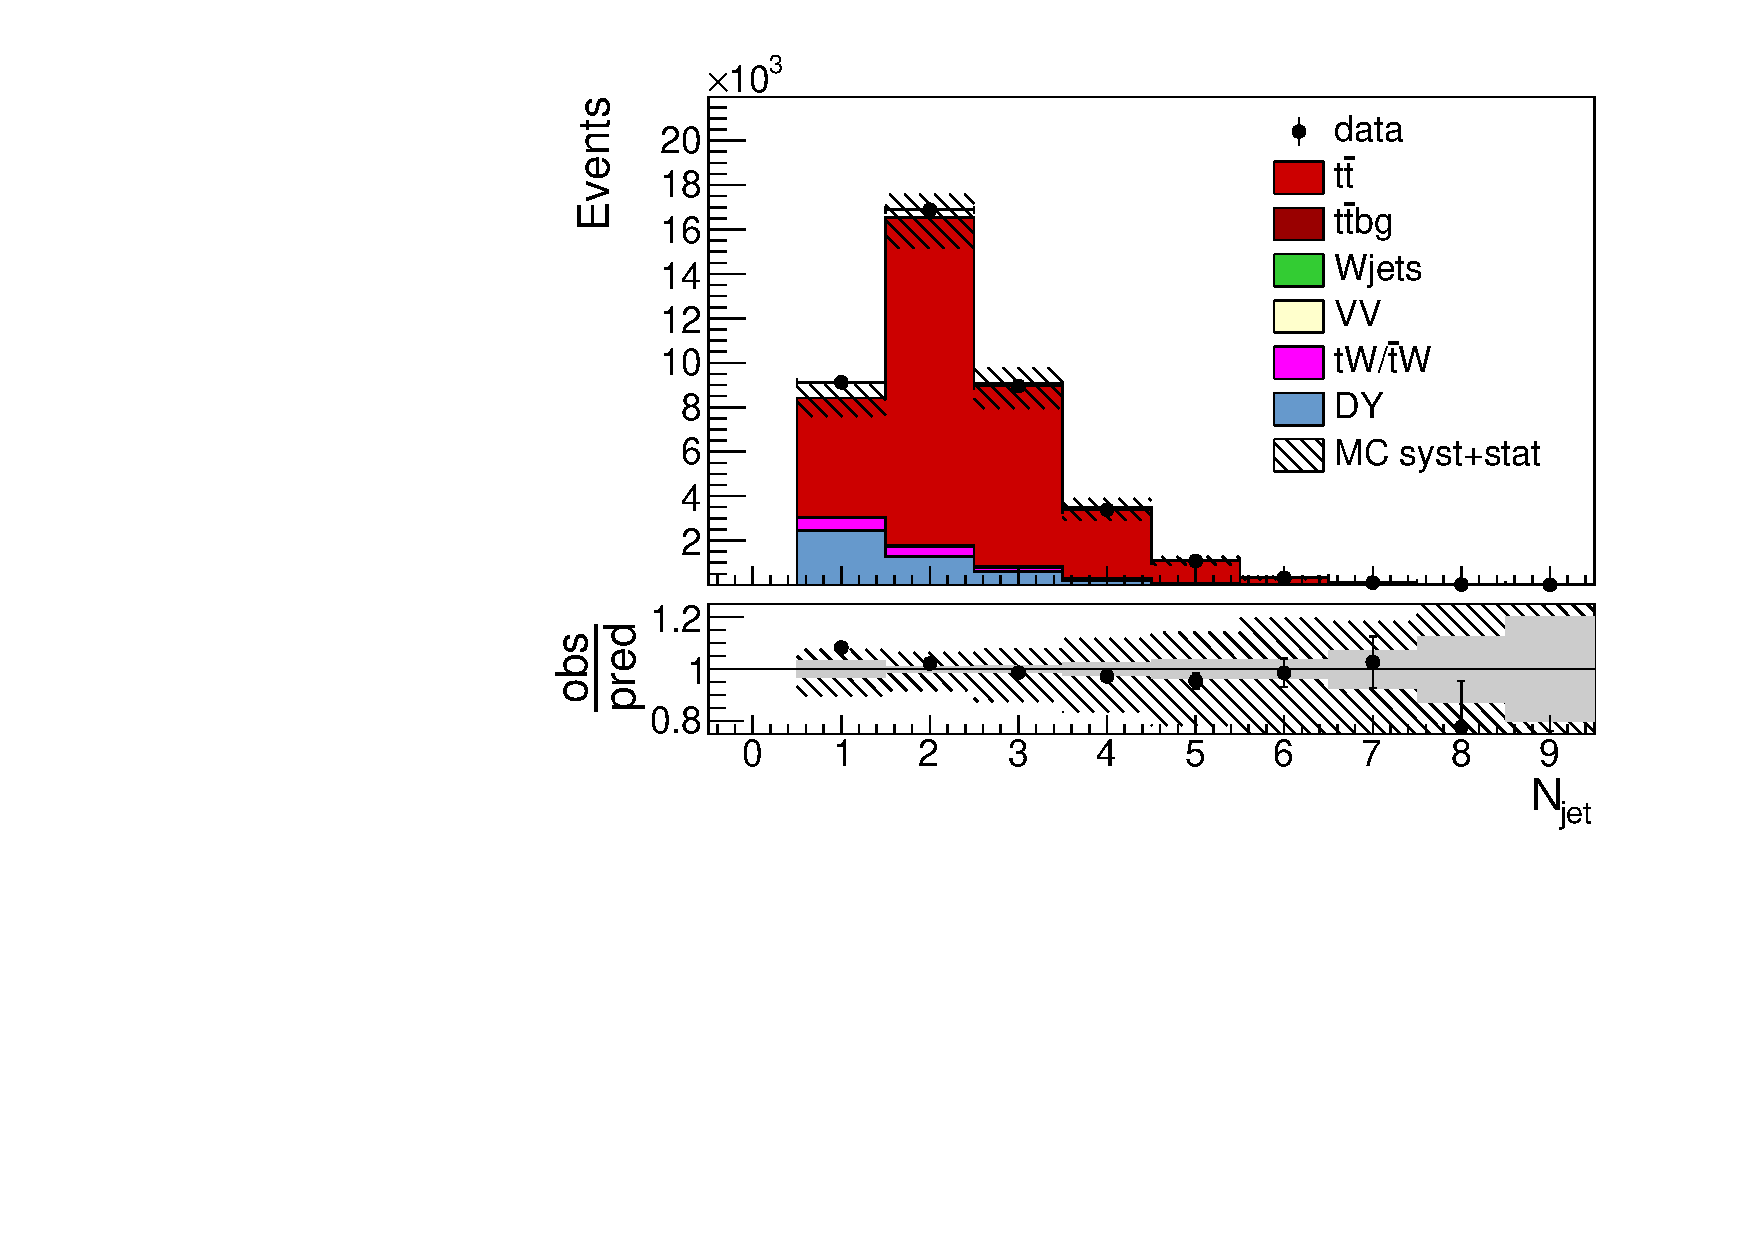
\includegraphics{CrossSection/Figures/ControlPlots/ee_sysnom/selected_jets_multi_step_8.pdf}}
    \caption{Number of jets \emu (upper left), \mumu (upper right) and \ee (lower row) decay channels.
        The events are shown after the
        event selection.  The hatched
        bands correspond to the total uncertainty on the sum of the
        predicted yields, excluding luminosity and background
        normalization uncertainties. 
        The ratios of data to the sum of the predicted yields are
        shown in the bottom panel of each figure. The solid gray band
        represents the contribution of the statistical uncertainty.}  
       \label{fig:xsec_jets_ctrplots}
  \end{center}
\end{figure}

The number of b-tagged jets for all three channels is shown in Figure~\ref{fig:xsec_bjets_ctrplots}.
Events with zero b-tagged jets are rejected for the same-flavor channels.
A significant amount of \ttbar signal events contain zero b-tagged jets, due to the comparably low efficiency to identify a jet containing a b quark.
However, the small amount of background events containing one or more b-tagged jet indicates the low probability to wrongly identify a jet as b-tagged.
The main remaining background contribution with one or more b-tagged jet in the \emu channel are events which contain a b quark from the top-quark decay.
In the same-flavor channel Drell-Yan events contribute significantly as well.
The behavior of the data is well modeled by the simulation in all three channels.

As shown in the figures, variables relating to (b-tagged) jets provide discrimination between signal and background. Hence these variables
are used to further separate signal and background

\begin{figure}[htbp!]
  \begin{center}
    \resizebox{0.48 \textwidth}{!}{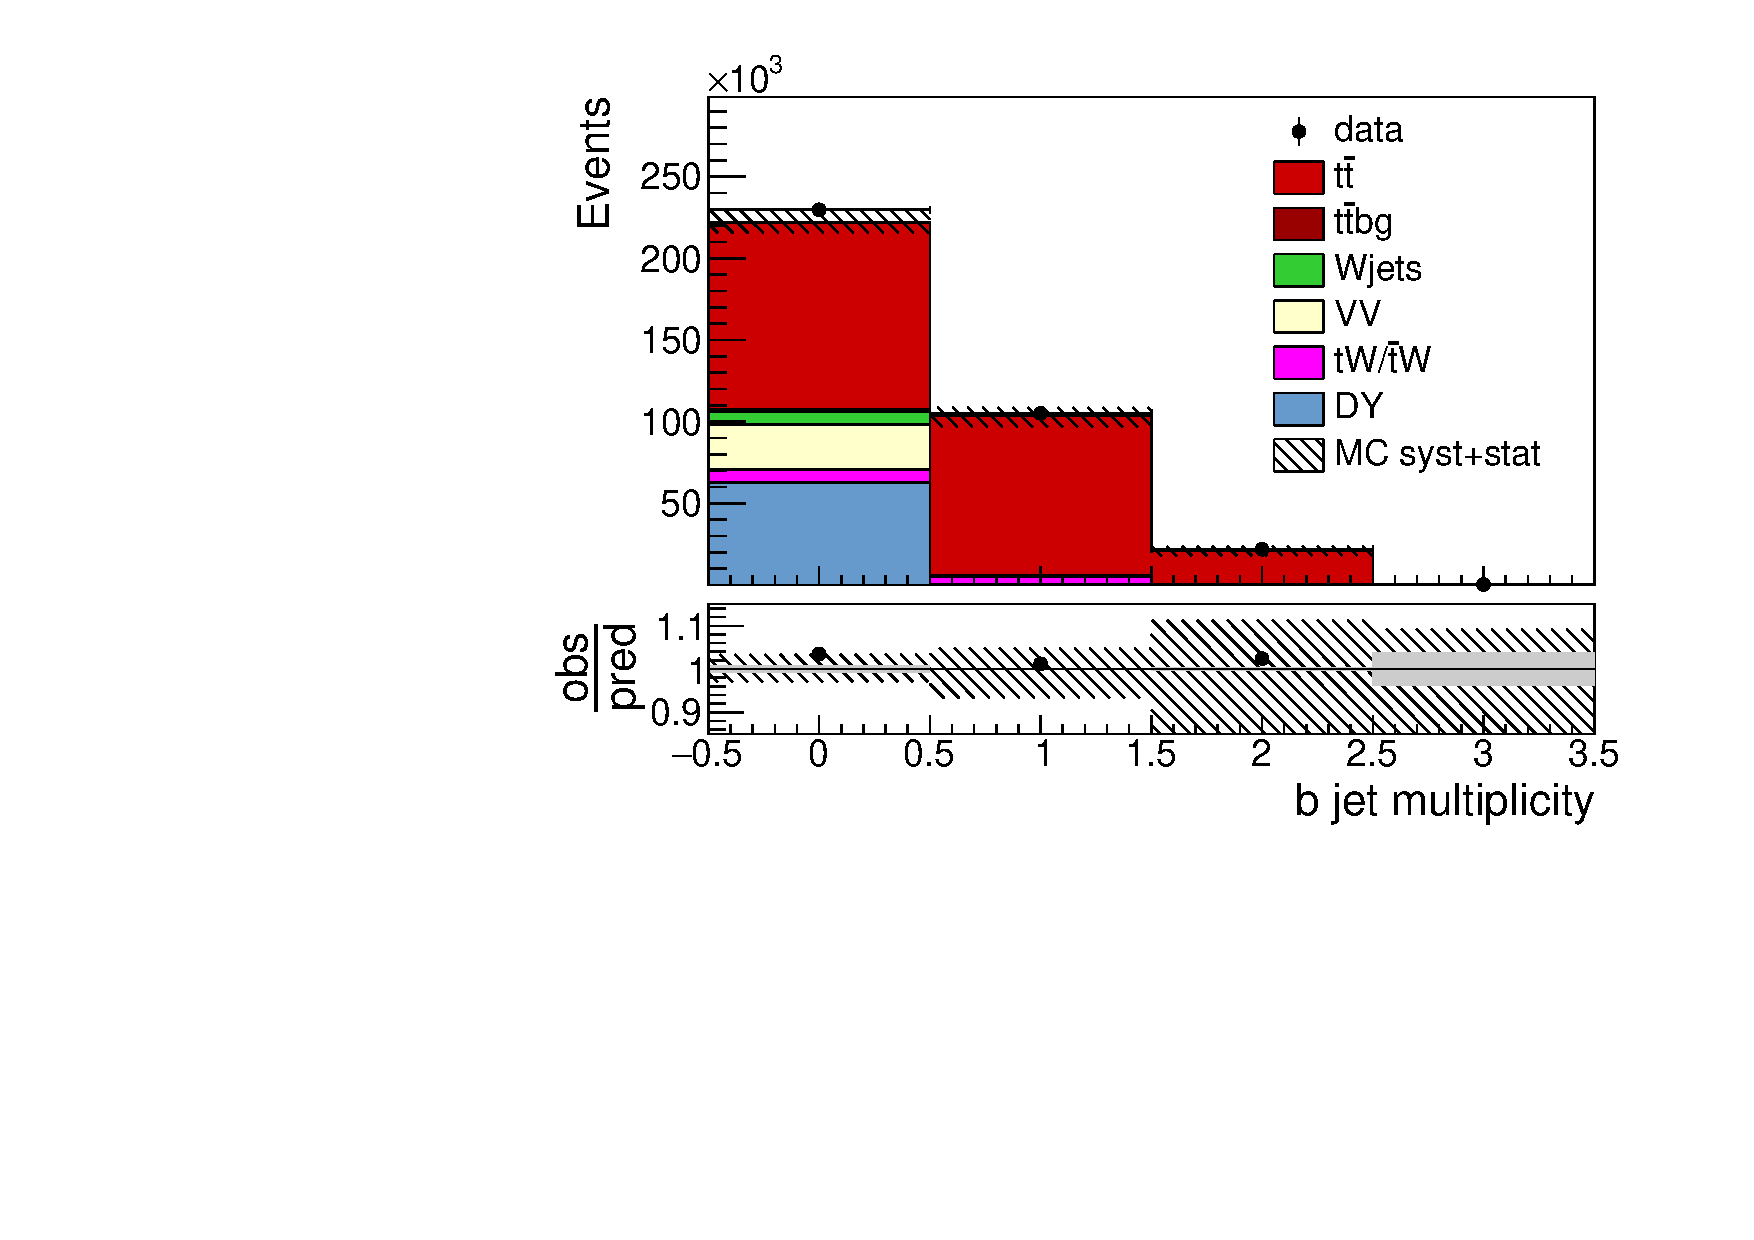
\includegraphics{CrossSection/Figures/ControlPlots/emu_sysnom/selected_b-jet_multi_step_8.pdf}}
    \resizebox{0.48 \textwidth}{!}{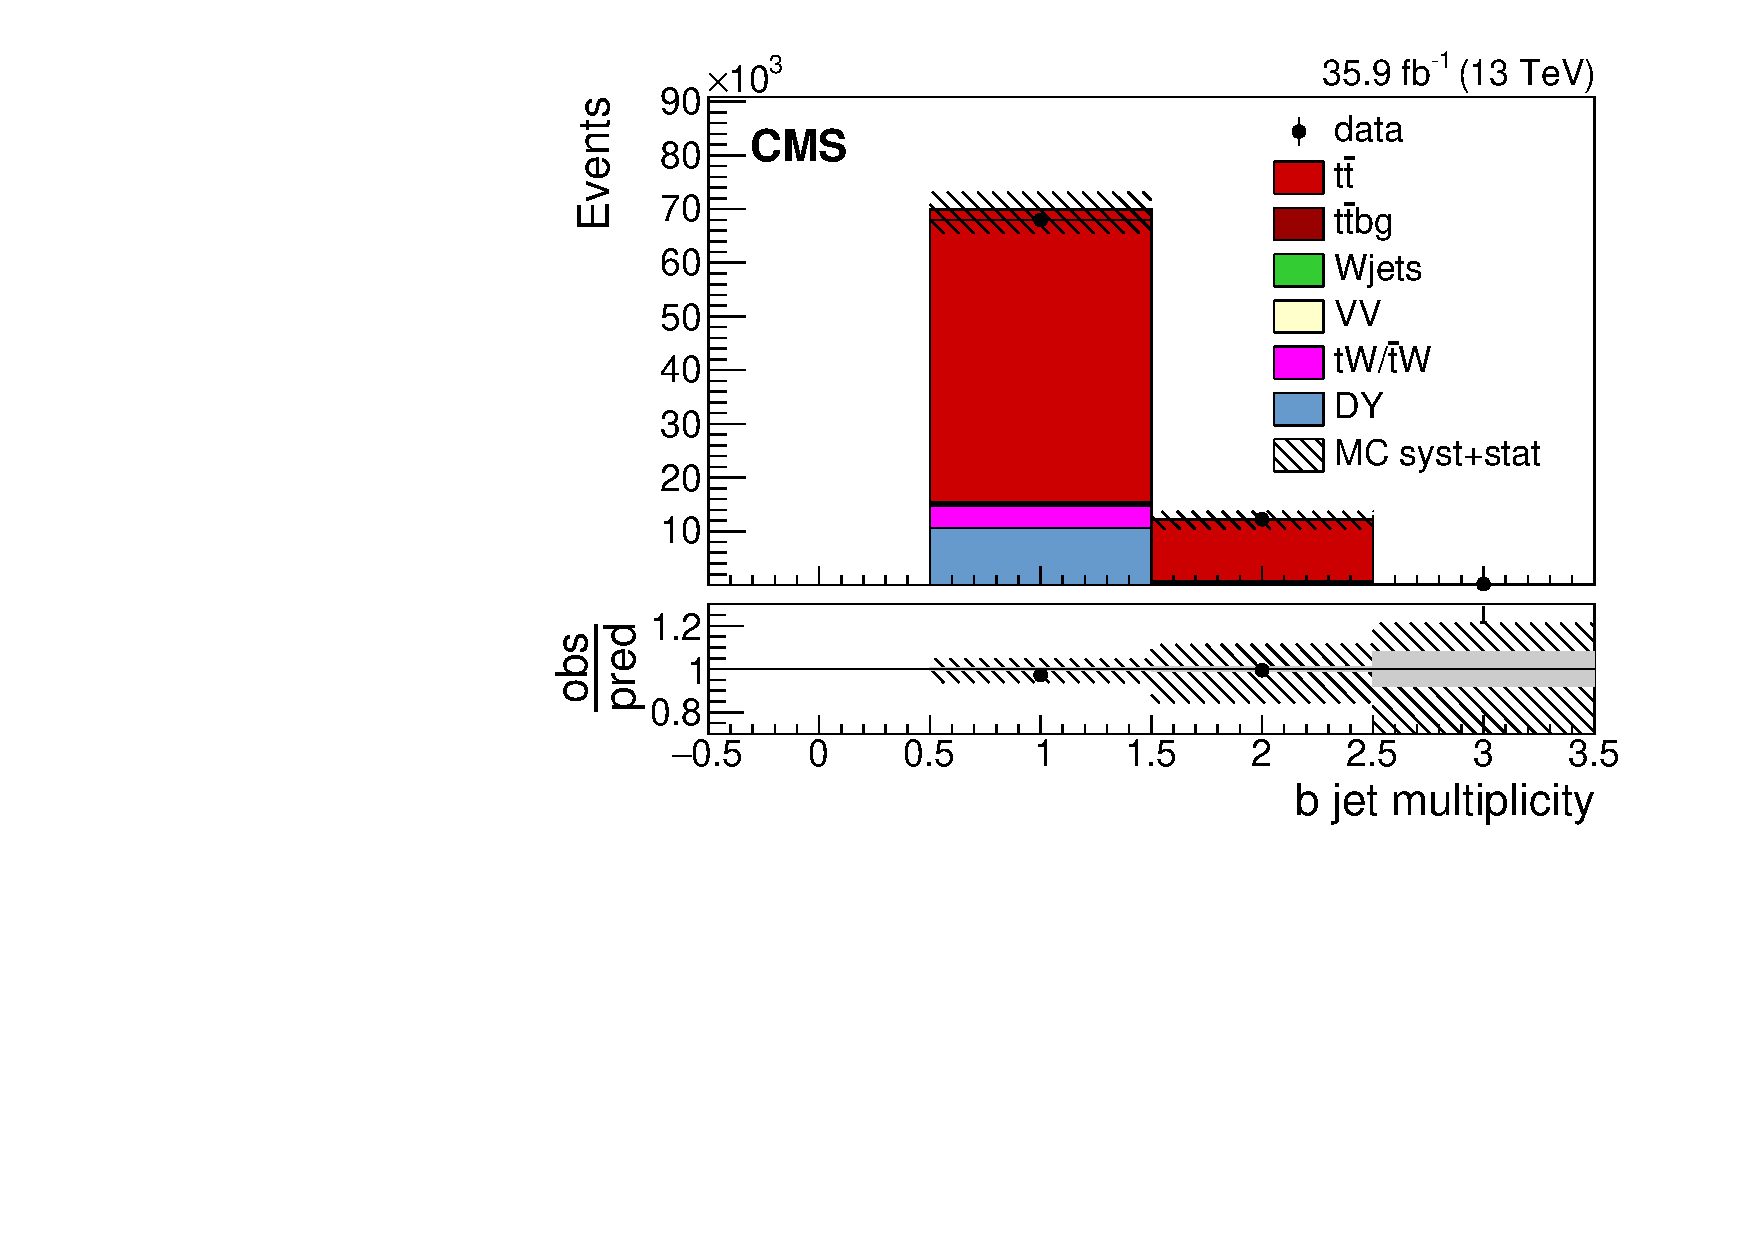
\includegraphics{CrossSection/Figures/ControlPlots/mumu_sysnom/selected_b-jet_multi_step_8.pdf}}
    \resizebox{0.48 \textwidth}{!}{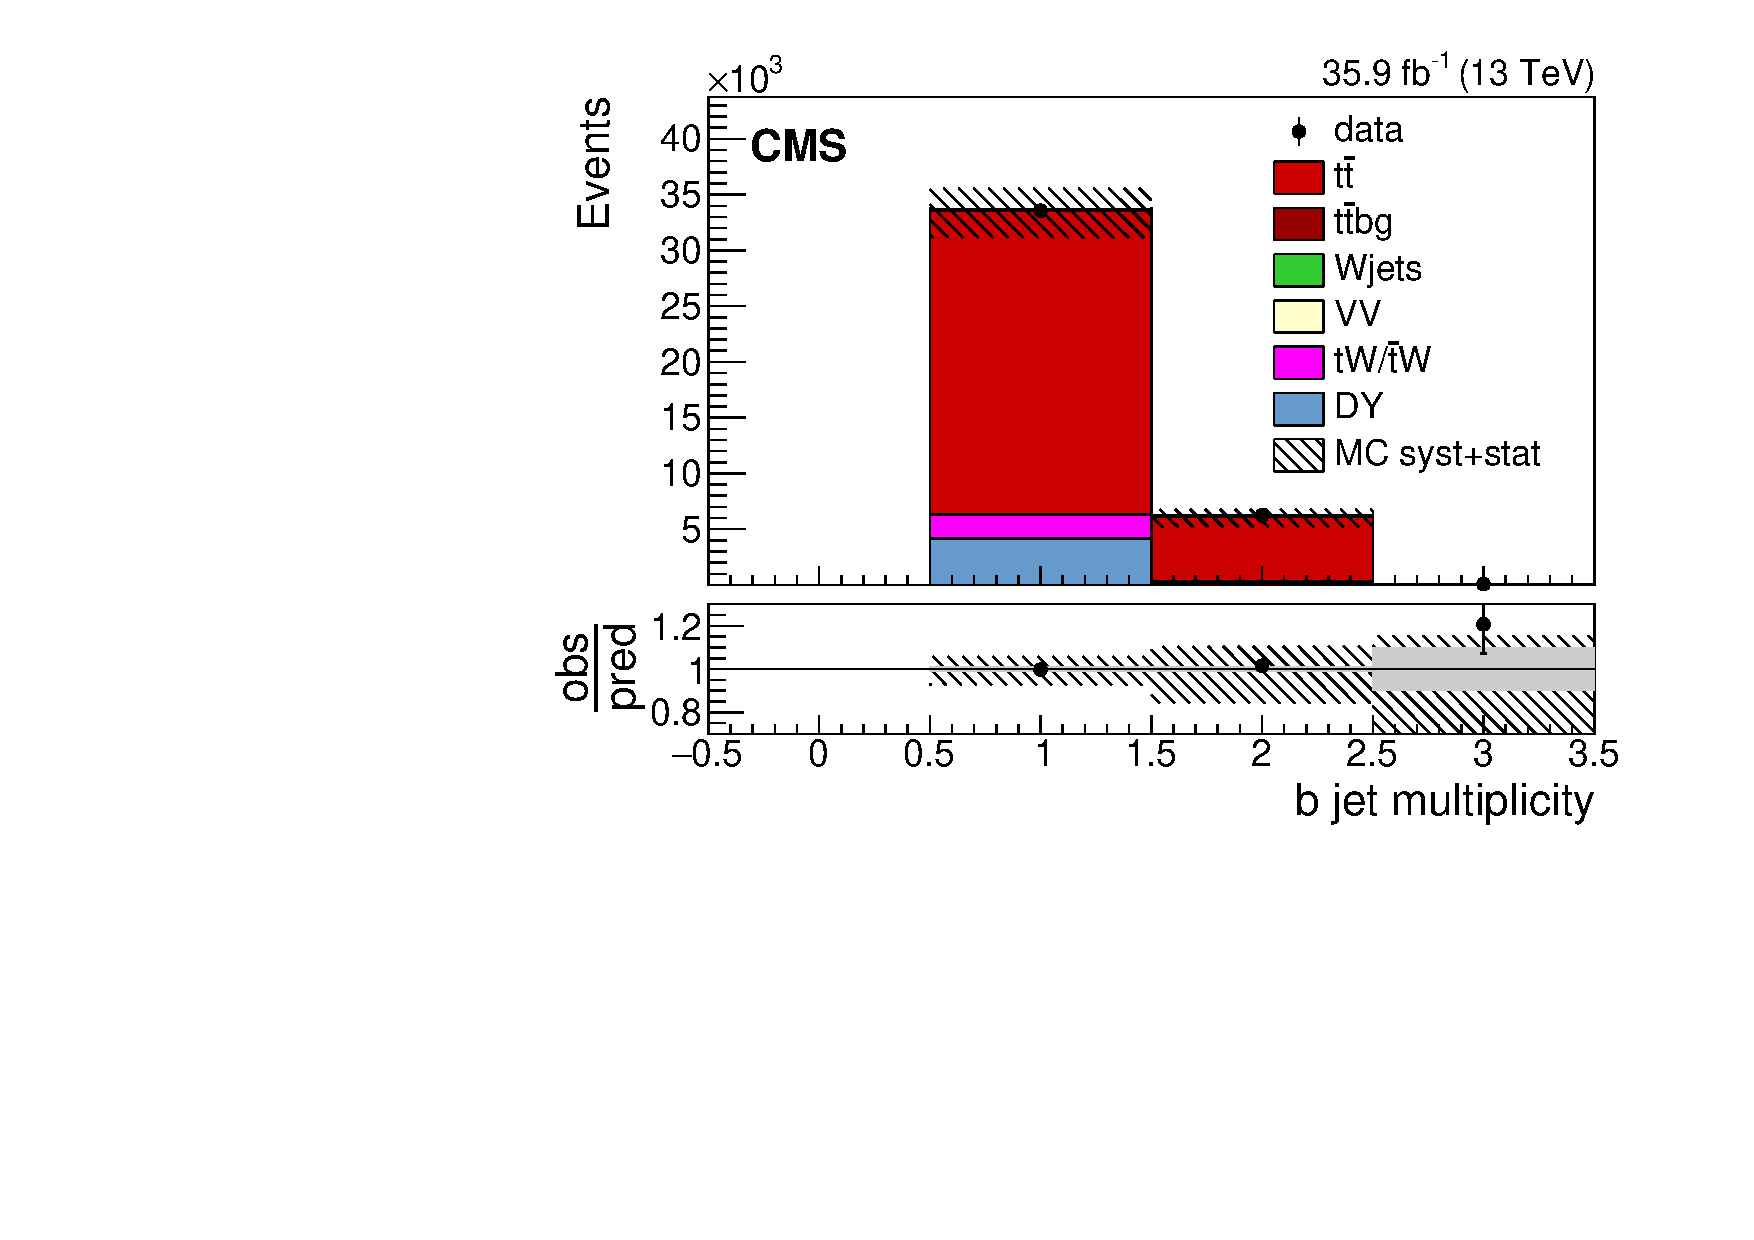
\includegraphics{CrossSection/Figures/ControlPlots/ee_sysnom/selected_b-jet_multi_step_8.pdf}}
    \caption{Number of b-tagged jets \emu (upper left), \mumu (upper right) and \ee (lower row) decay channels.
        The events are shown after the
        event selection.  The hatched
        bands correspond to the total uncertainty on the sum of the
        predicted yields, excluding luminosity and background
        normalization uncertainties. 
        The ratios of data to the sum of the predicted yields are
        shown in the bottom panel of each figure. The solid gray band
        represents the contribution of the statistical uncertainty.}  
       \label{fig:xsec_bjets_ctrplots}
  \end{center}
\end{figure}


The invariant mass of the dilepton system is shown in Figure~\ref{fig:xsec_ctrplots_mll} for the \emu channel and depending on the number of b-tagged jets (for zero, one and two or more b-tagged jets).
The distribution for signal events has a broad maximum in the region of $60-100 \; \GeV$ with long tails up to $300 \; \GeV$.
Drell-Yan events show the expected peak at the mass of the Z boson.


In most distributions the data are well modeled by the simulation. In regions where the modeling is poor, the discrepancies are accounted for with systematic uncertainties.

\begin{figure}[htbp!]
  \begin{center}
    \resizebox{0.48 \textwidth}{!}{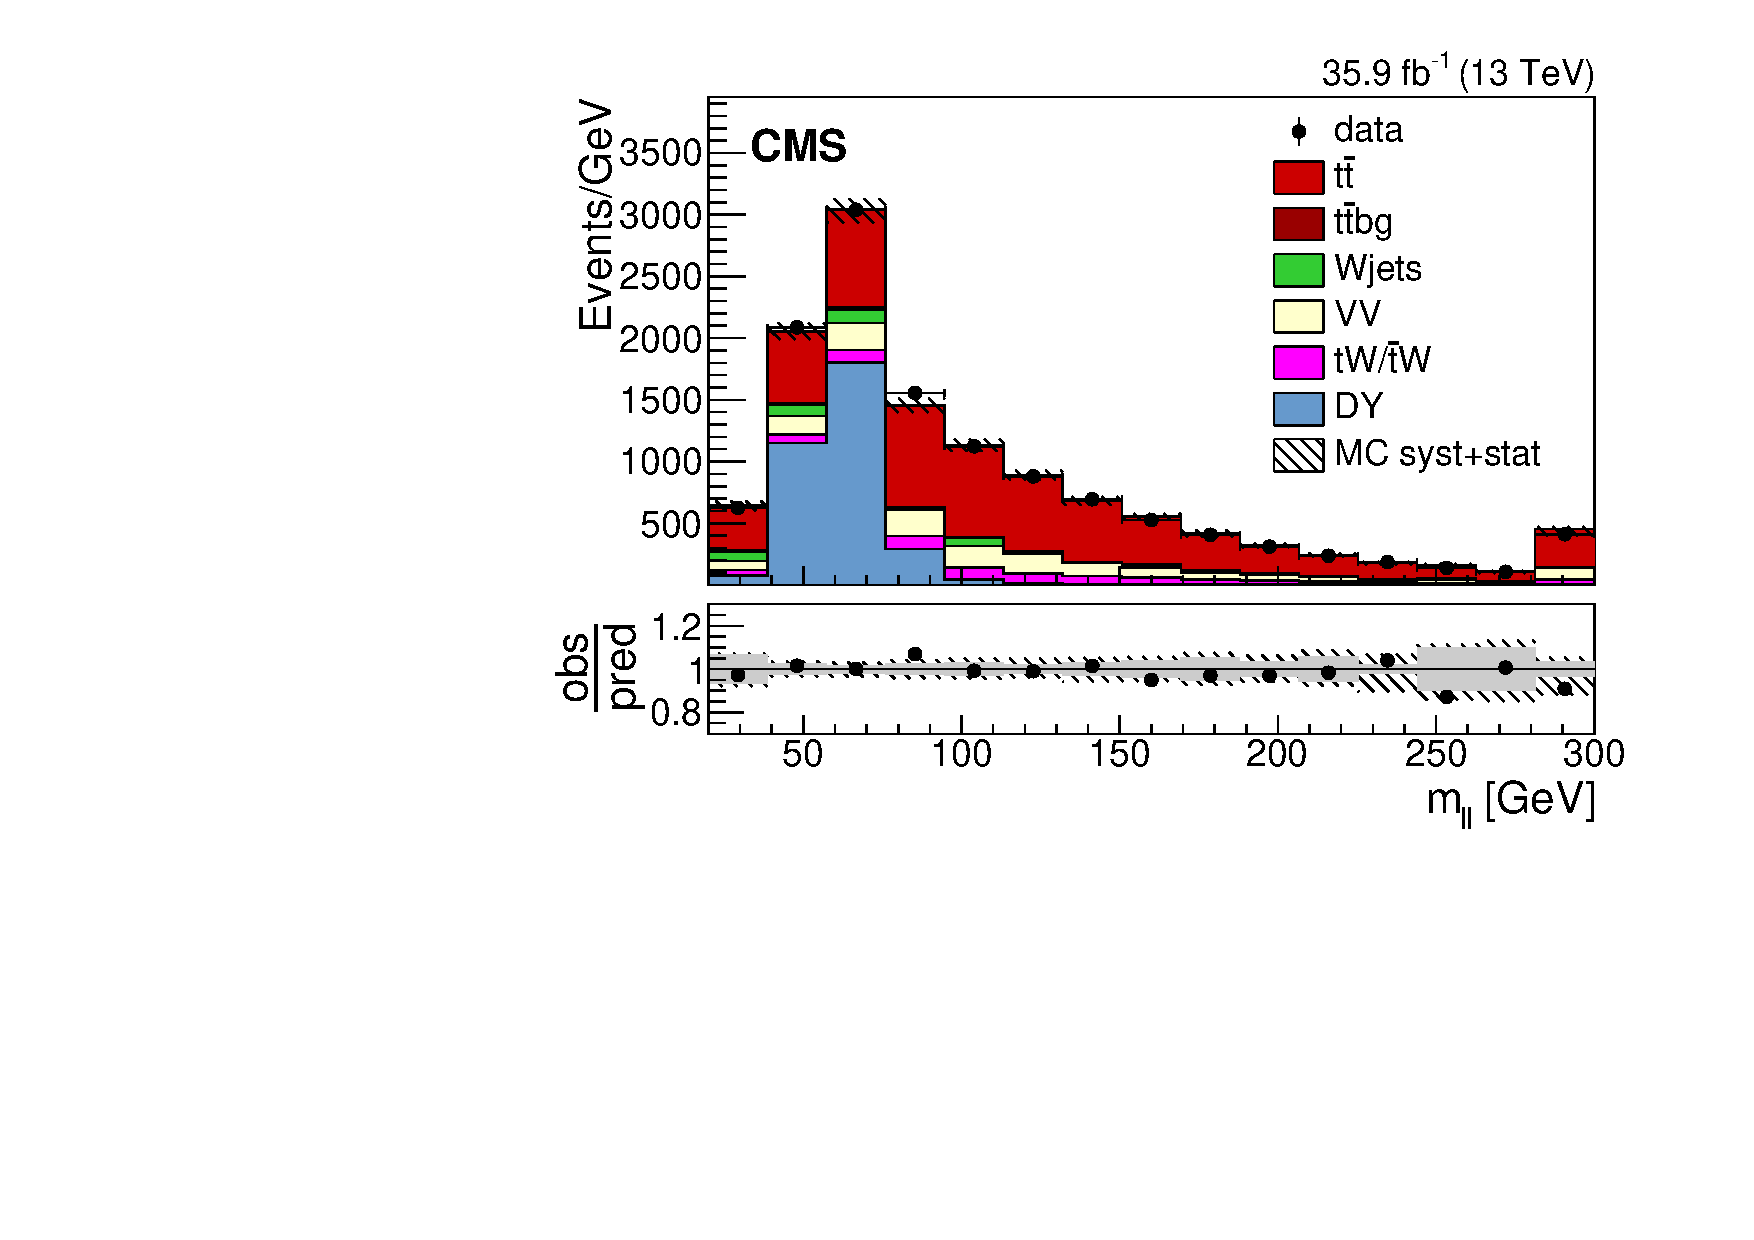
\includegraphics{CrossSection/Figures/ControlPlots/emu_sysnom/mll_0_b-jets_step_8.pdf}}
    \resizebox{0.48 \textwidth}{!}{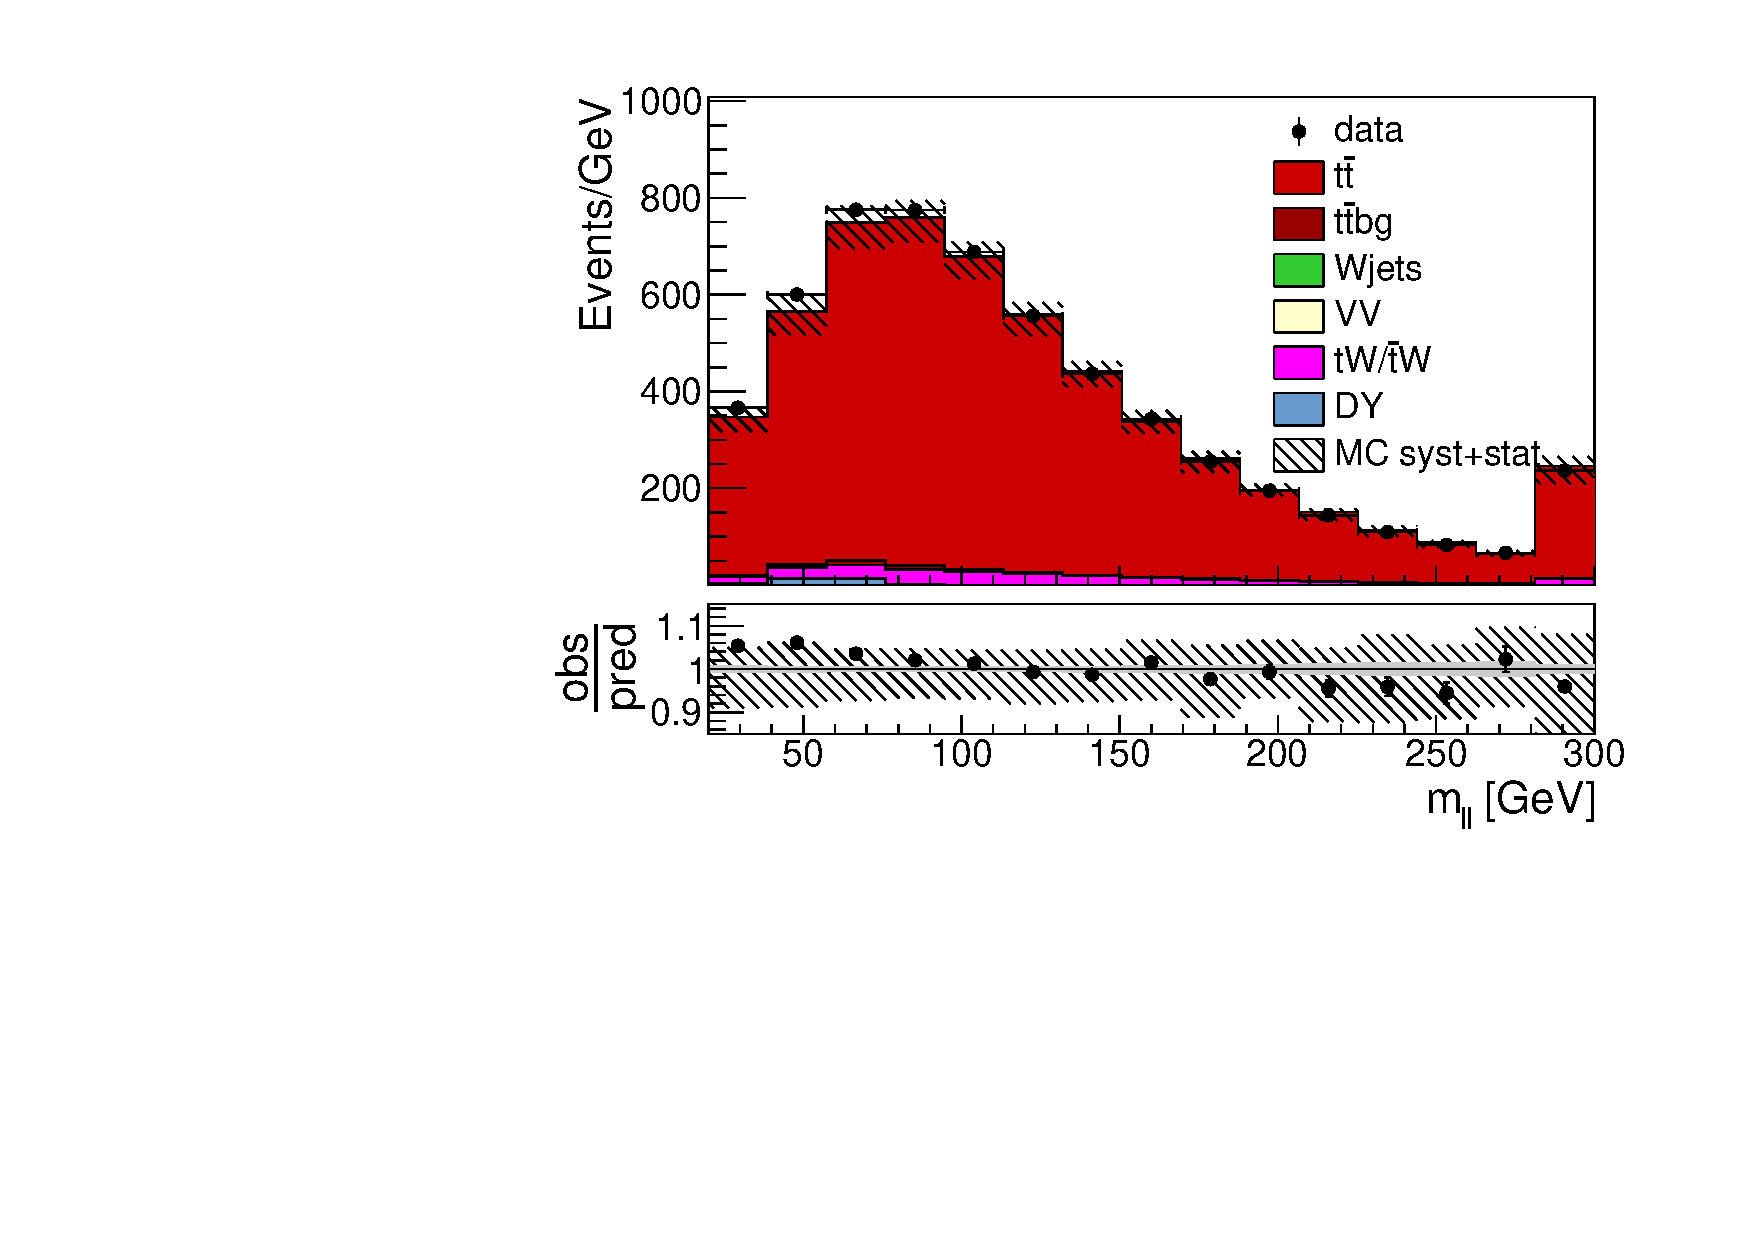
\includegraphics{CrossSection/Figures/ControlPlots/emu_sysnom/mll_1_b-jets_step_8.pdf}}
    \resizebox{0.48 \textwidth}{!}{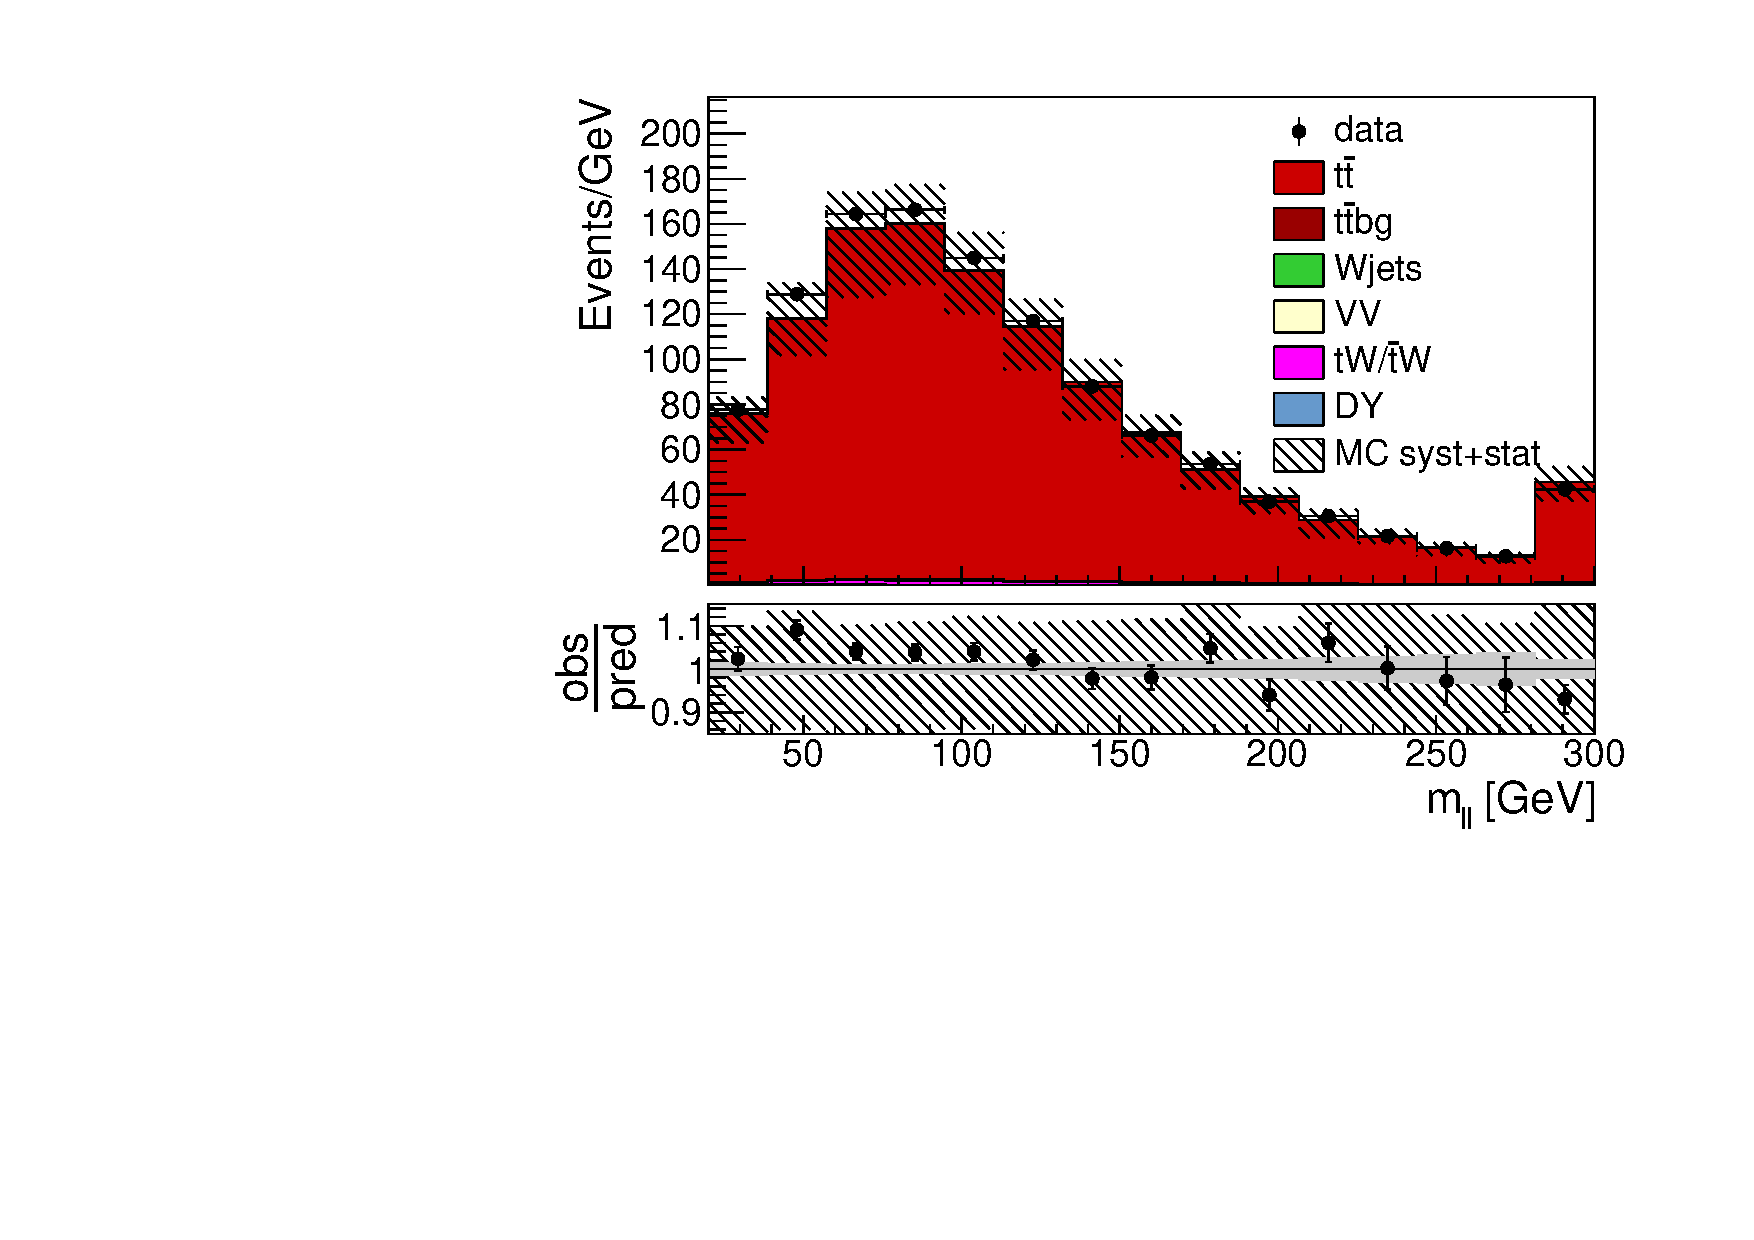
\includegraphics{CrossSection/Figures/ControlPlots/emu_sysnom/mll_2_b-jets_step_8.pdf}} \\
      \caption{Invariant mass of the dilepton system with zero (upper left), one (upper right) and two (lower row) b-tagged 
      jets in the \emu channel. The hatched
        bands correspond to the total uncertainty on the sum of the
        predicted yields, excluding luminosity and background
        normalization uncertainties. 
        The ratios of data to the sum of the predicted yields are
        shown in the bottom panel of each figure. The solid gray band
        represents the contribution of the statistical uncertainty.}  
       \label{fig:xsec_ctrplots_mll}
  \end{center}
\end{figure}



\section{Choice of event categories and template distributions}
\label{sec:xsec_templates}

The events are categorized by lepton flavor, number of b-tagged jets and number of non b-tagged jets. This leads to 28 different categories.
In each category a template distribution is used to constrain the uncertainties.
An overview is given in Table~\ref{tab:xsec_templates}.

\begin{table}[htbp!]
\begin{center}
\caption{Table of the template distributions chosen for the fit. They are listed for each of the three decay channels and are further split according to the number
of b-tagged jets and additional non b-tagged jets.~\label{tab:xsec_templates}}
\begin{tabular}{c|l|l|l|l}
Number of b jets                      & Number of add. jets&   \multicolumn{3}{c}{Decay channel}                  \\
                                      &                    & \emu channel      & \mumu channel   & \ee channel \\
\hline
\multirow{3}{*}{0 or $\geq 3$ b jets} & 0 add. jets        & event yield       & -               & -            \\
                                      & 1 add. jets        & \pt (1st jet)     & -               & -            \\
                                      & 2 add. jets        & \pt (2nd jet)     & -               & -            \\
                                      & $\geq 3$ add. jets & \pt (trail. jet)  & -               & -            \\ 
\hline    
\multirow{3}{*}{1 b jet}              & 0 add. jets        & event yield       & event yield     & event yield  \\
                                      & 1 add. jets        & \pt (1st jet)     & event yield     & event yield  \\
                                      & 2 add. jets        & \pt (2nd jet)     & event yield     & event yield   \\
                                      & $\geq 3$ add. jets & \pt (trail. jet)  & event yield     & event yield   \\ 
\hline
\multirow{3}{*}{2 b jets}              & 0 add. jets        & event yield       & event yield     & event yield  \\
                                      & 1 add. jets        & \pt (1st jet)     & \pt (1st jet)   & \pt (1st jet) \\
                                      & 2 add. jets        & \pt (2nd jet)     & \pt (2nd jet)   & \pt (2nd jet) \\
                                      & $\geq 3$ add. jets & event yield   & event yield & event yield  \\                                 


\end{tabular}
\end{center}
\end{table}

In order to maximize the separation between signal and background the events are divided according to the number of b-tagged jets.
There are three categories of events corresponding to $N_{b-jet}=1$, $N_{b-jet}=2$ or $N_{b-jet}=0$ and $N_{b-jet} \geq 3$.
This categorization also allows determining the efficiency to find a b-tagged jet in a signal event using the topology of \ttbar decays.
Since each of the top quarks decays into a W boson and a b quark, every \ttbar event should contain two jets originating from b quarks.
Decays of a top quark to a W boson and a light quark are considered negligible.
Therefore, the number of \ttbar events with less than two b-tagged jets can be used to measure the efficiency to select a b-tagged jet.

In this way, the b-tagging efficiency is determined independently for data and simulation (see Section~\ref{sec:xsec_stat}). The efficiency of the b-tagging algorithm is independent of the lepton flavor and is  assumed to be the same for all \ttbar decay channels.
The in-situ measurement of the b-tagging efficiency in the phase space of the \ttbar cross section measurement reduces the impact of the uncertainty on the b-tagging efficiency.
The b-tagging efficiency can also be measured in an independent measurement, but measuring it in-situ is preferable to avoid extrapolation to a different phase space.

Besides the number of b-tagged jets, the number of light (non b-tagged) jets is one of the main discriminators between \ttbar and background events.
Events containing a top quark pair tend to have a larger amount of additional jets from final state radiation.
Events are split according to the number of light jets for one, two and zero or more than two jets.
In each event the \pt of the trailing light jet is chosen as template distribution.
Together with the \pt of the light jets, their multiplicity is sensitive to the systematic uncertainty on the response of the jet reconstruction and
the systematic uncertainties introduced by theoretical assumptions in the simulation.

The separation of events into the \emu, \mumu and \ee channels is explained in Section~\ref{sec:xsec_sel}. The \ttbar cross section is assumed to be constant in all three decay channels. Any difference in branching 
ratio can be assumed to be described correctly in simulation.
By simultaneously fitting the three channels with the two uncorrelated lepton identification efficiencies $\epsilon_e$ and $\epsilon_\mu$ the nuisance parameters related to the two efficiencies are correlated. 
The relation between the number of \ttbar events in each dilepton channel ($s_{\emu}$, $s_{ee}$ and $s_{\mu\mu}$), the ttbar cross section (\stt) and the lepton 
efficiencies  is shown in simplified form in Equation~\ref{eq:xsec_lepsplit}.
\begin{eqnarray}
s_{e \mu}  &\propto& \stt \epsilon_{e} \epsilon_{\mu}  \\
s_{ee}  &\propto&  \stt \epsilon_{e}^2  \\
s_{\mu \mu}  &\propto&  \stt \epsilon_{\mu}^2
\label{eq:xsec_lepsplit}.
\end{eqnarray}
These relations can be rewritten as: 

\begin{equation}
\frac{s_{\mu\mu}}{s_{ee}} \propto \frac{\epsilon_{\mu}^2}{\epsilon_{e}^2} \hspace{0.8cm} \frac{s_{\mu\mu}}{s_{e\mu}} \propto \frac{\epsilon_{\mu}}{\epsilon_{e}}
\label{eq:xsec_lepeffs}
\end{equation}
By measuring $s_{\mu\mu}$ and $s_{ee}$ the efficiencies are constrained.
Since the uncertainties on the lepton efficiencies are uncorrelated before the fit, the constraints of the efficiency ratio suppress the larger of the two lepton efficiency uncertainties.
Here, prior to the fit, the muon identification uncertainty is smaller, and thus in the fit the single-electron identification uncertainty is constrained to that of the muon.

The final 28 templates are listed in Table~\ref{tab:xsec_templates} and shown in Figures 
~\ref{fig:xsec_emu_inputdistr},~\ref{fig:xsec_mumu_inputdistr} and~\ref{fig:xsec_ee_inputdistr} for the \emu, \mumu and \ee channel respectively.




\begin{figure}[htbp!]
  \begin{center}
    \resizebox{0.32 \textwidth}{!}{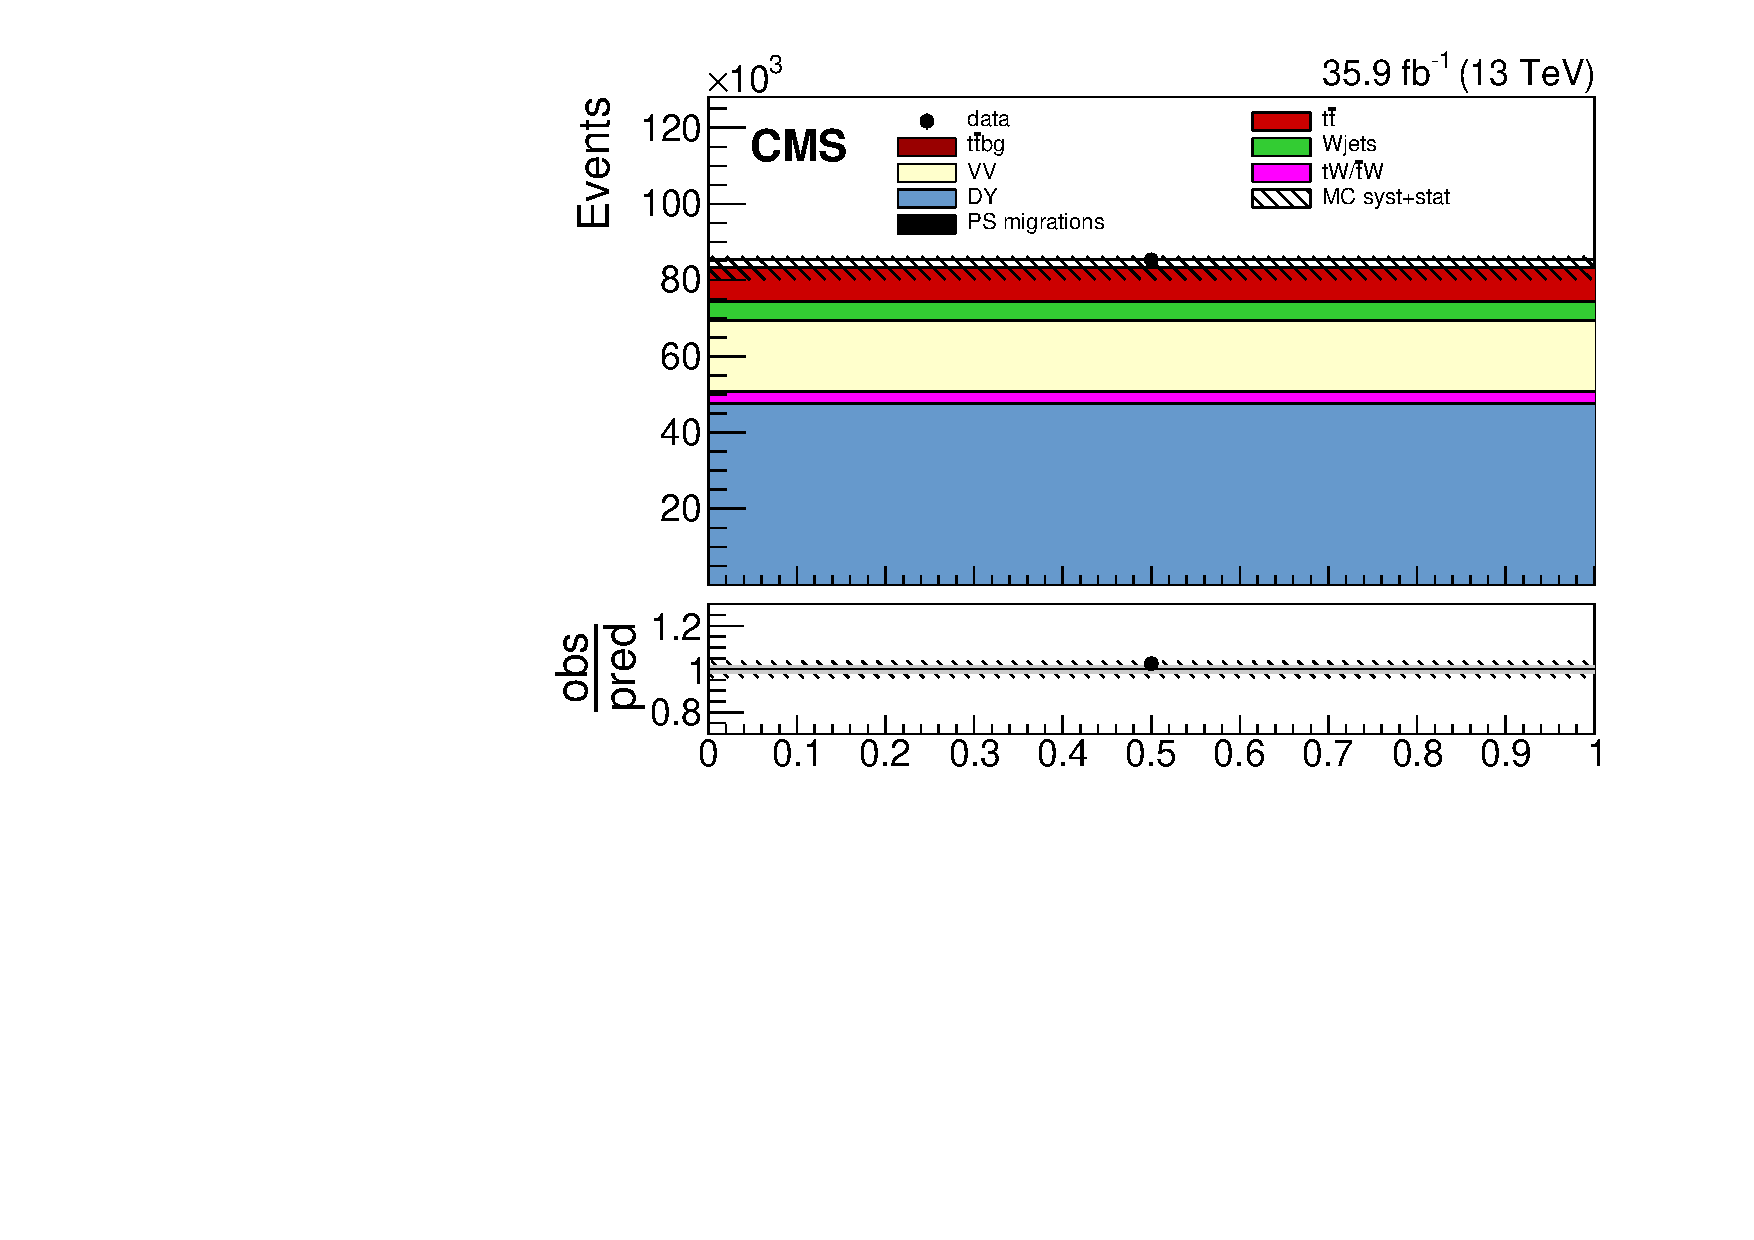
\includegraphics{CrossSection/Figures/ControlPlots/emu_sysnom/total_0_0_b-jets_step_8.pdf}}
    \resizebox{0.32 \textwidth}{!}{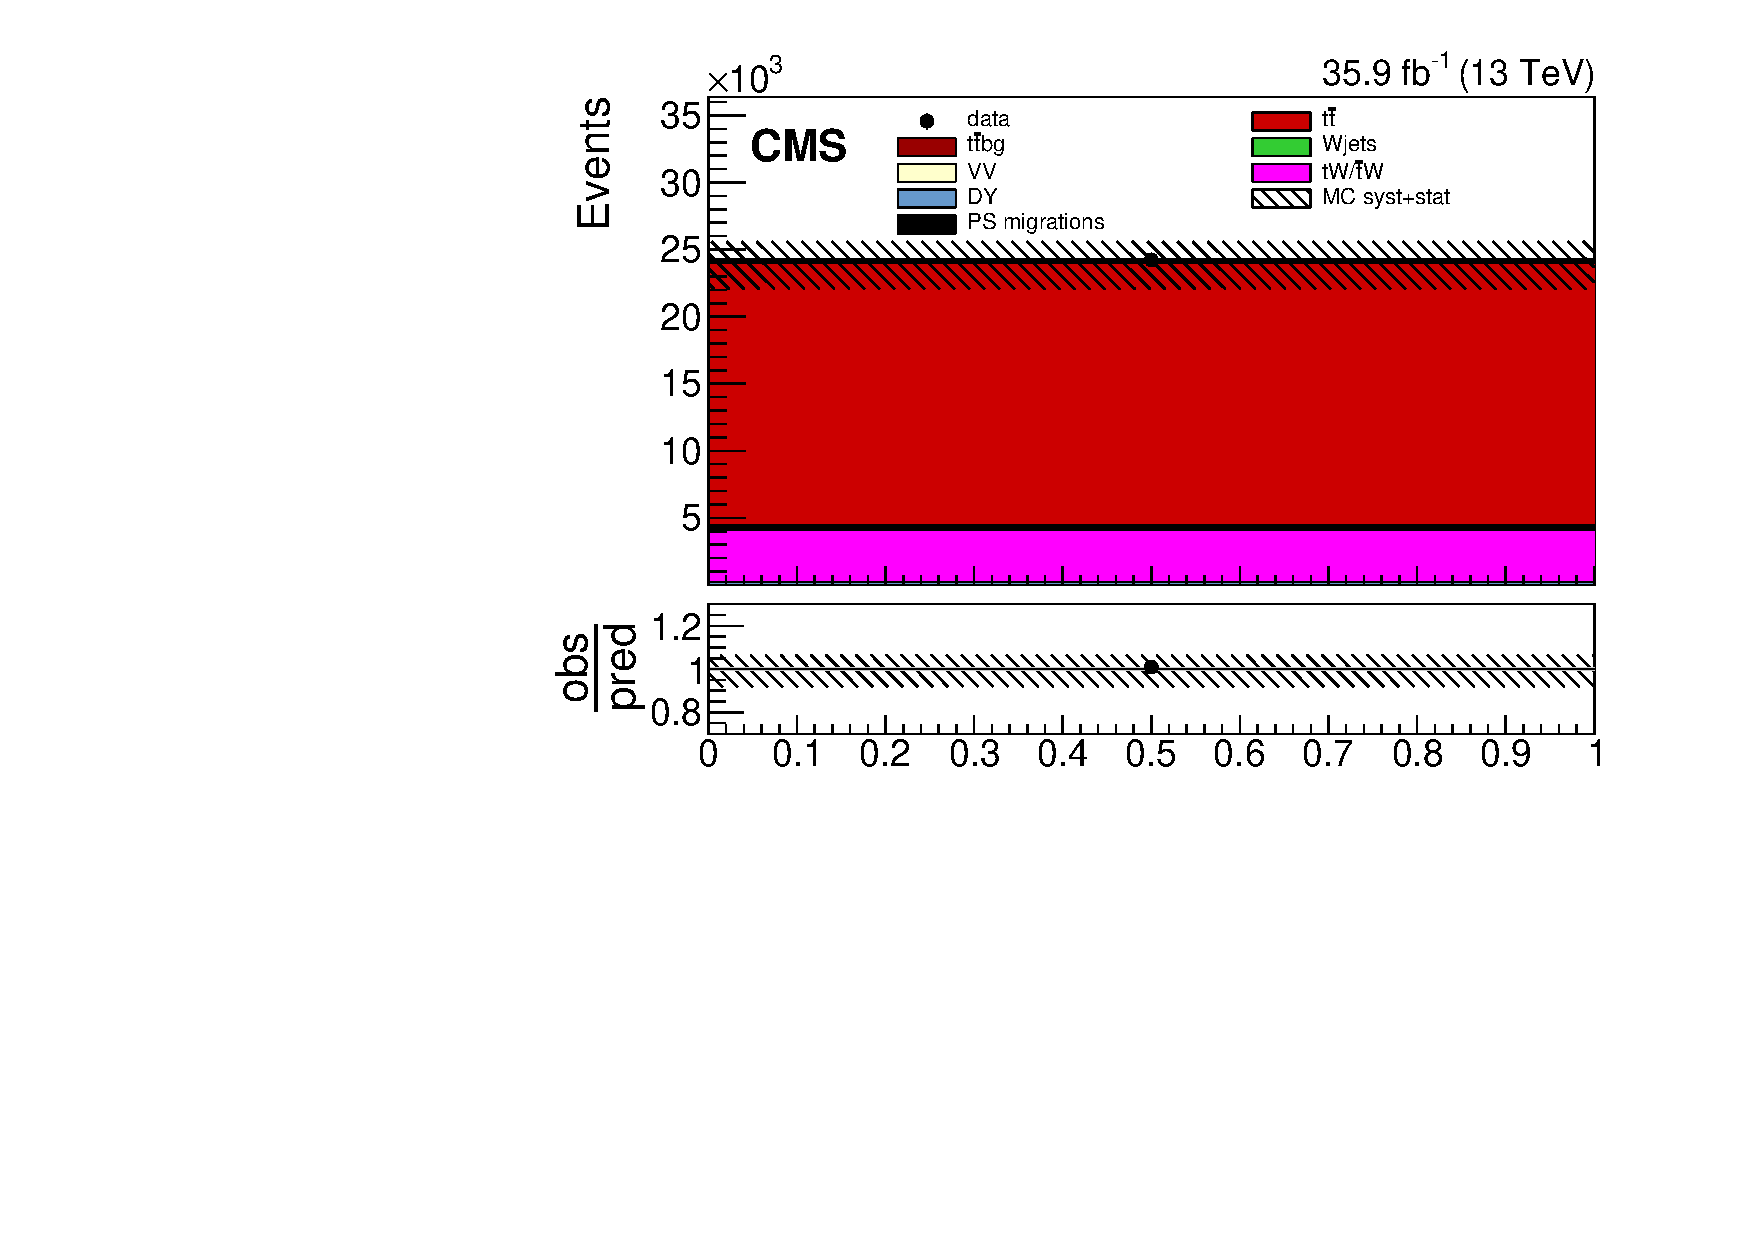
\includegraphics{CrossSection/Figures/ControlPlots/emu_sysnom/total_1_0_b-jets_step_8.pdf}}
    \resizebox{0.32 \textwidth}{!}{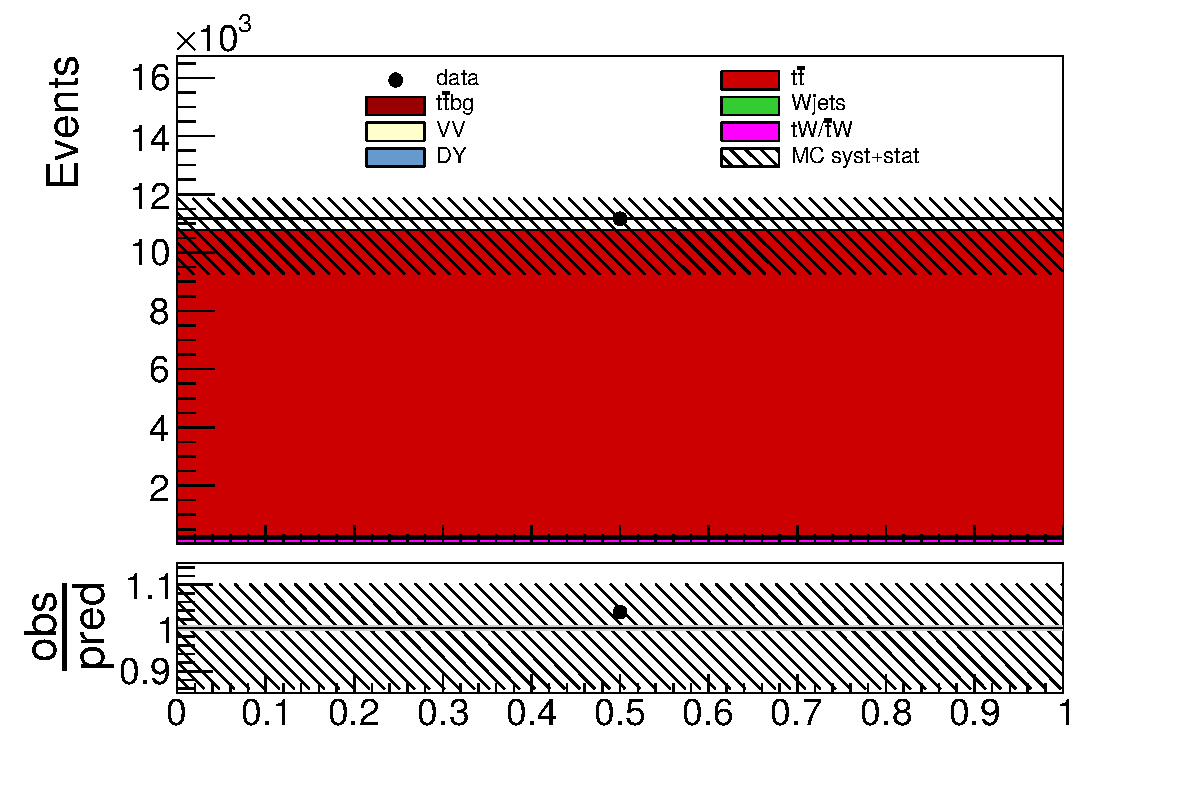
\includegraphics{CrossSection/Figures/ControlPlots/emu_sysnom/total_2_0_b-jets_step_8.pdf}}

    \resizebox{0.32 \textwidth}{!}{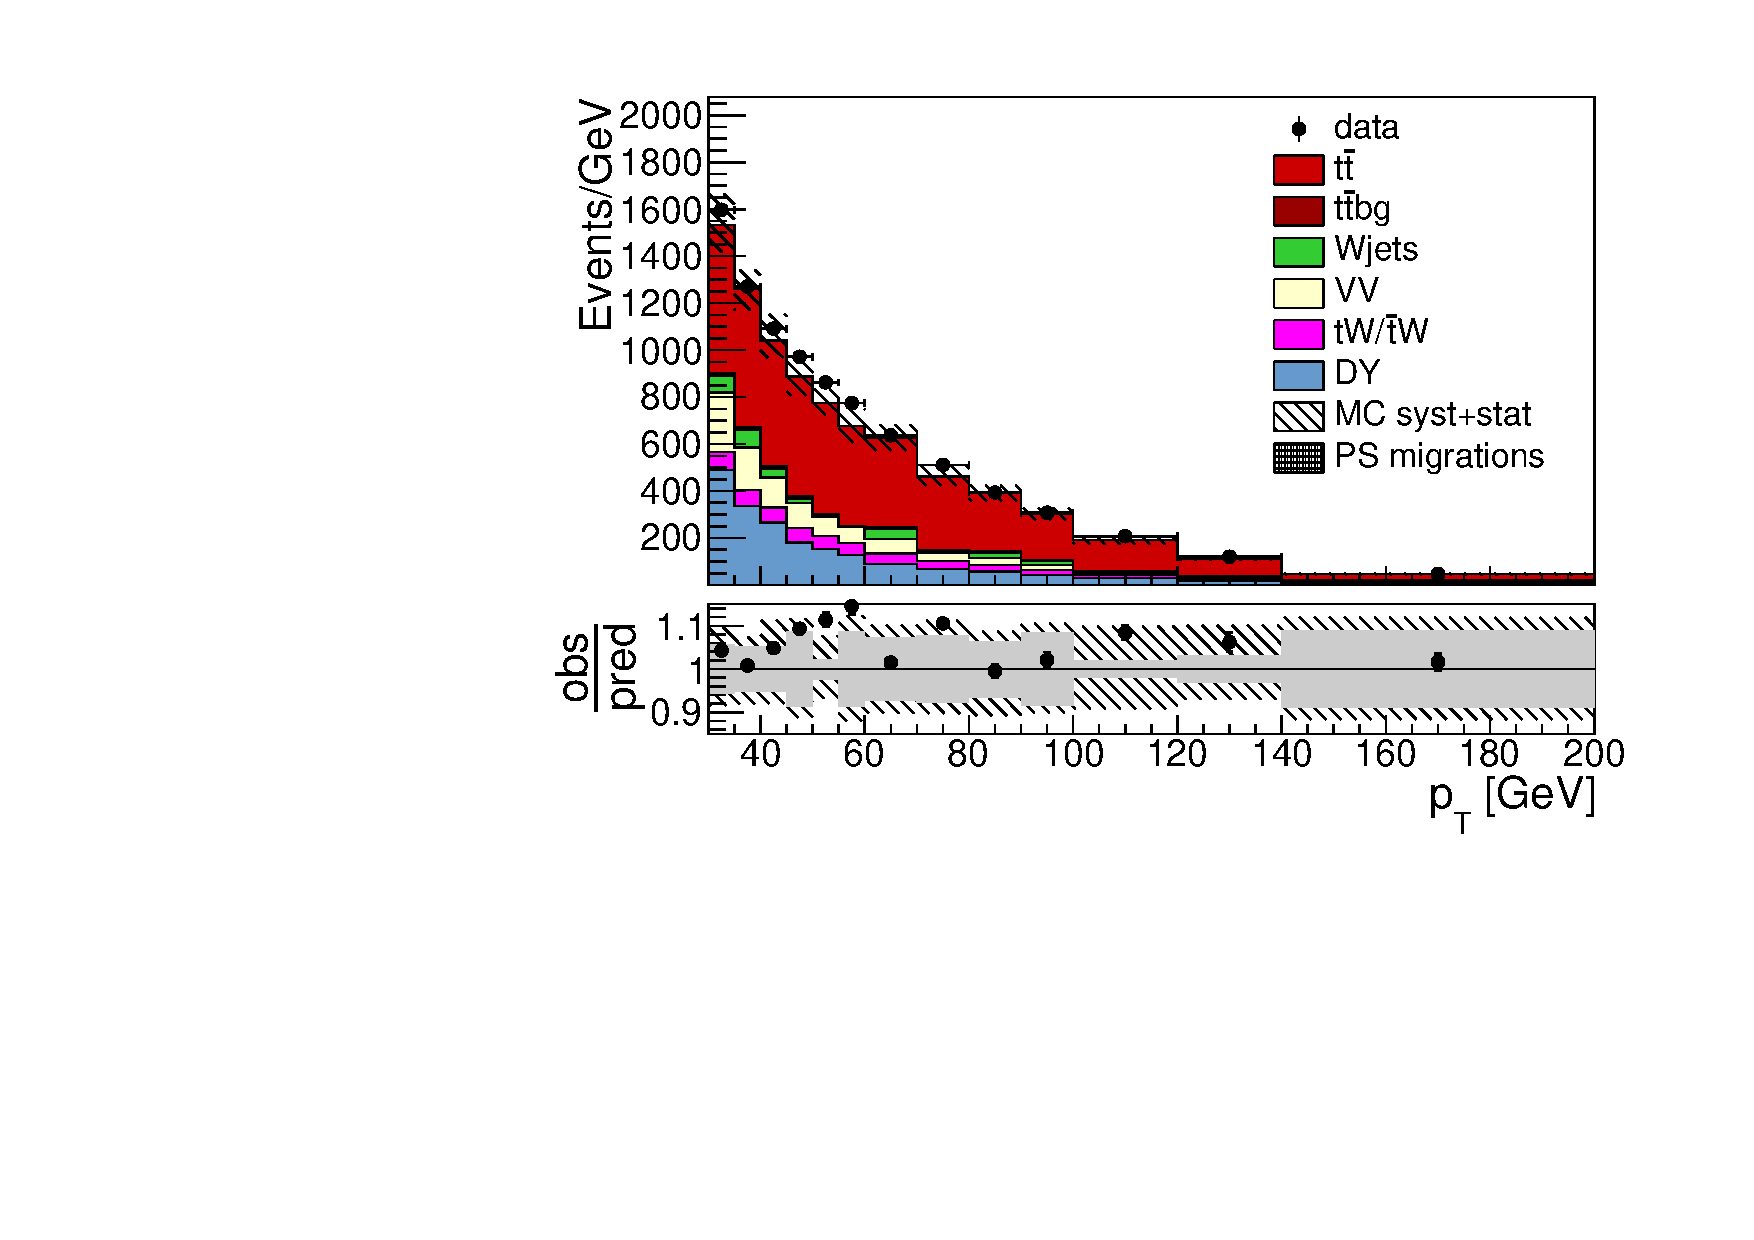
\includegraphics{CrossSection/Figures/ControlPlots/emu_sysnom/lead_jet_pt_0_1_b-jets_step_8.pdf}}
    \resizebox{0.32 \textwidth}{!}{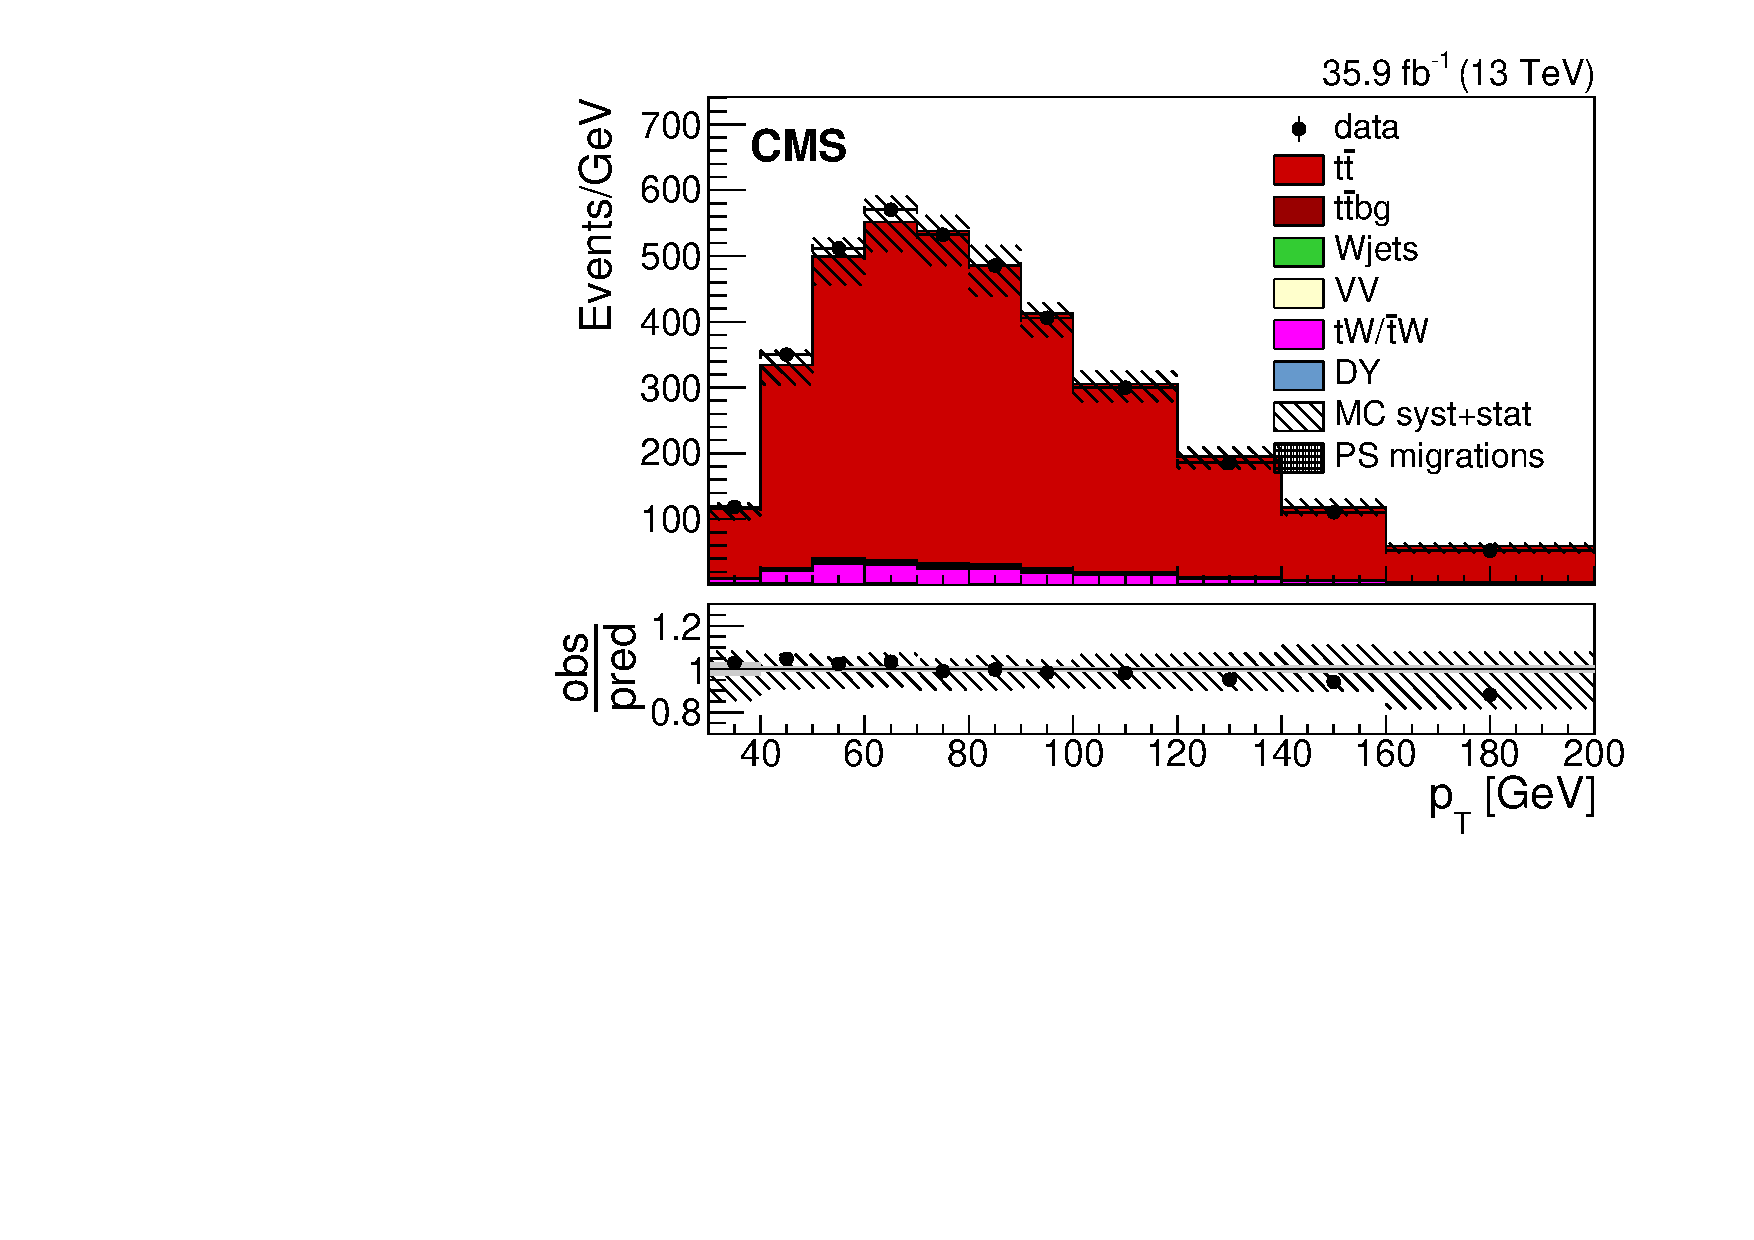
\includegraphics{CrossSection/Figures/ControlPlots/emu_sysnom/lead_jet_pt_1_1_b-jets_step_8.pdf}}
    \resizebox{0.32 \textwidth}{!}{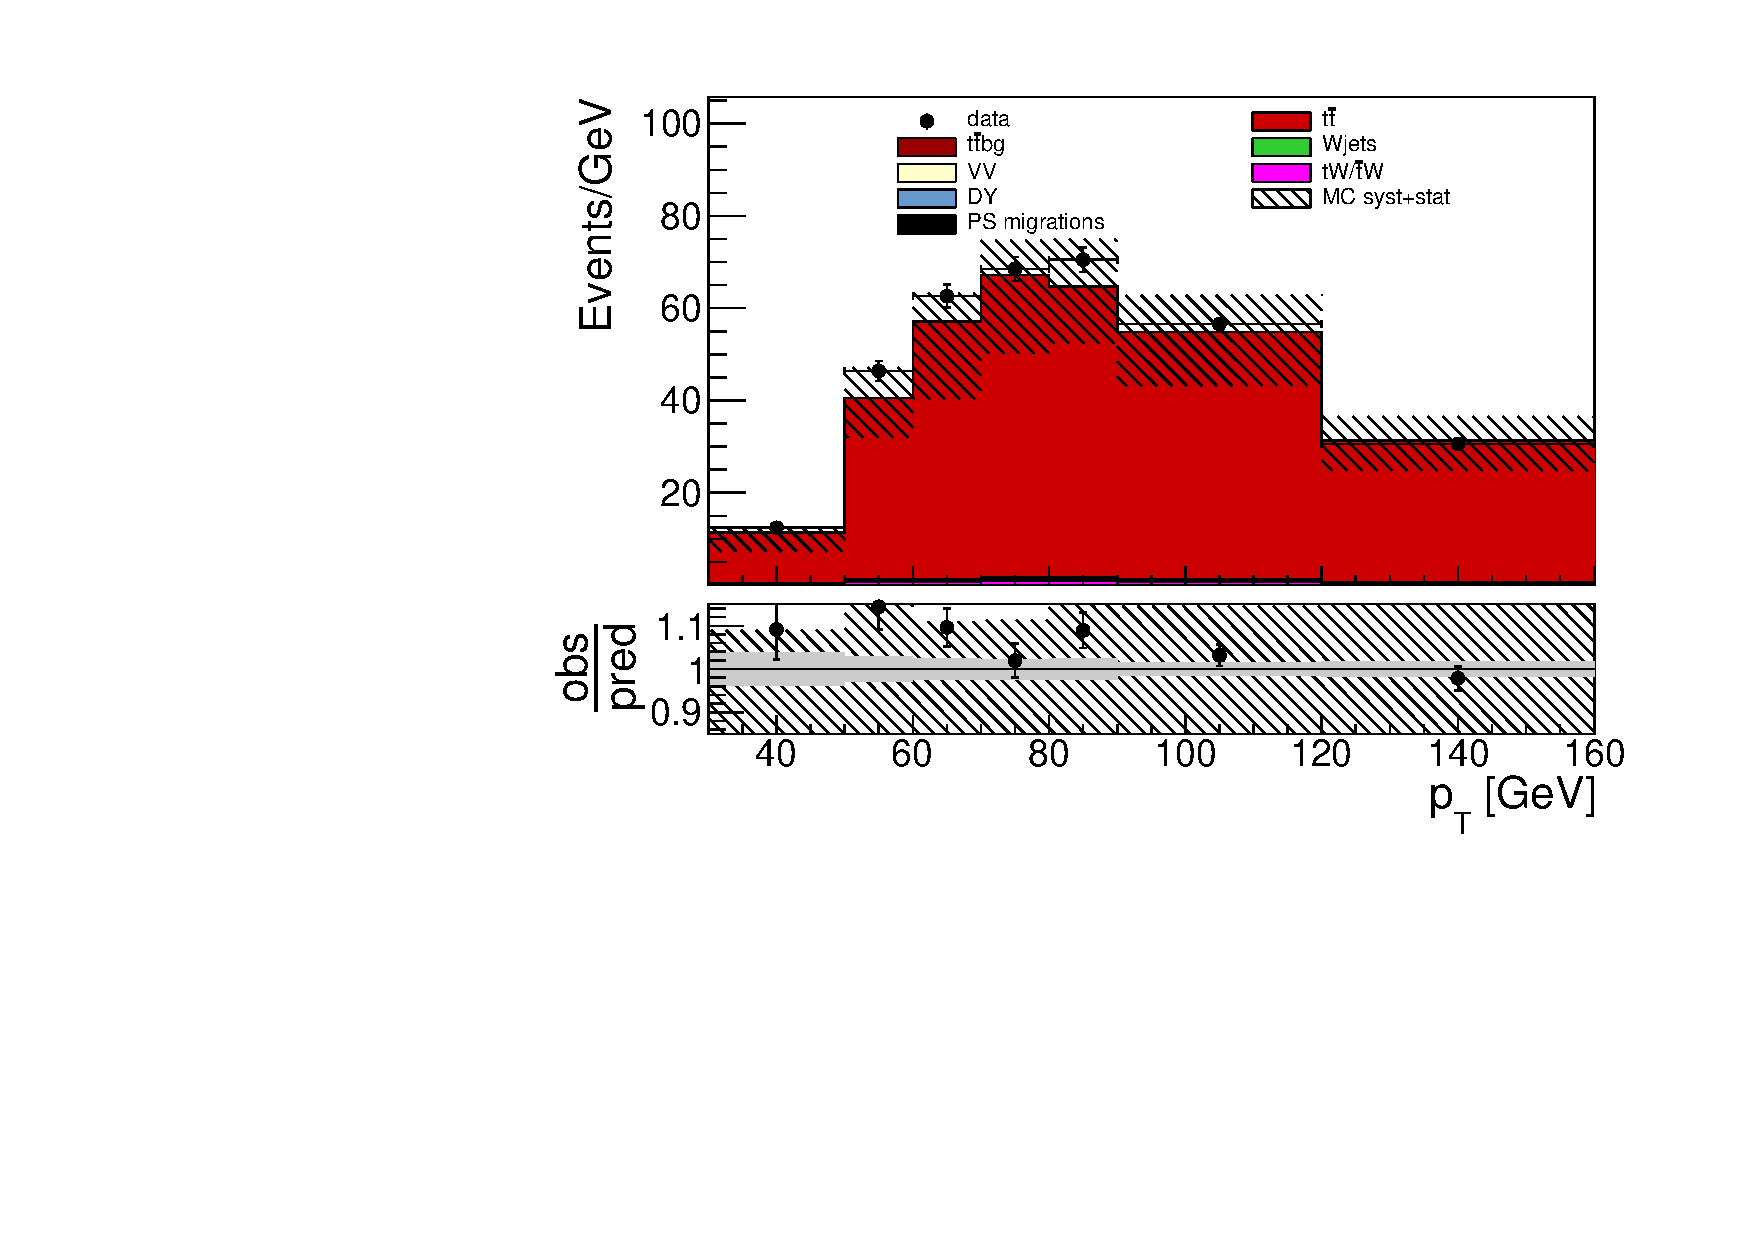
\includegraphics{CrossSection/Figures/ControlPlots/emu_sysnom/lead_jet_pt_2_1_b-jets_step_8.pdf}}
        
    \resizebox{0.32 \textwidth}{!}{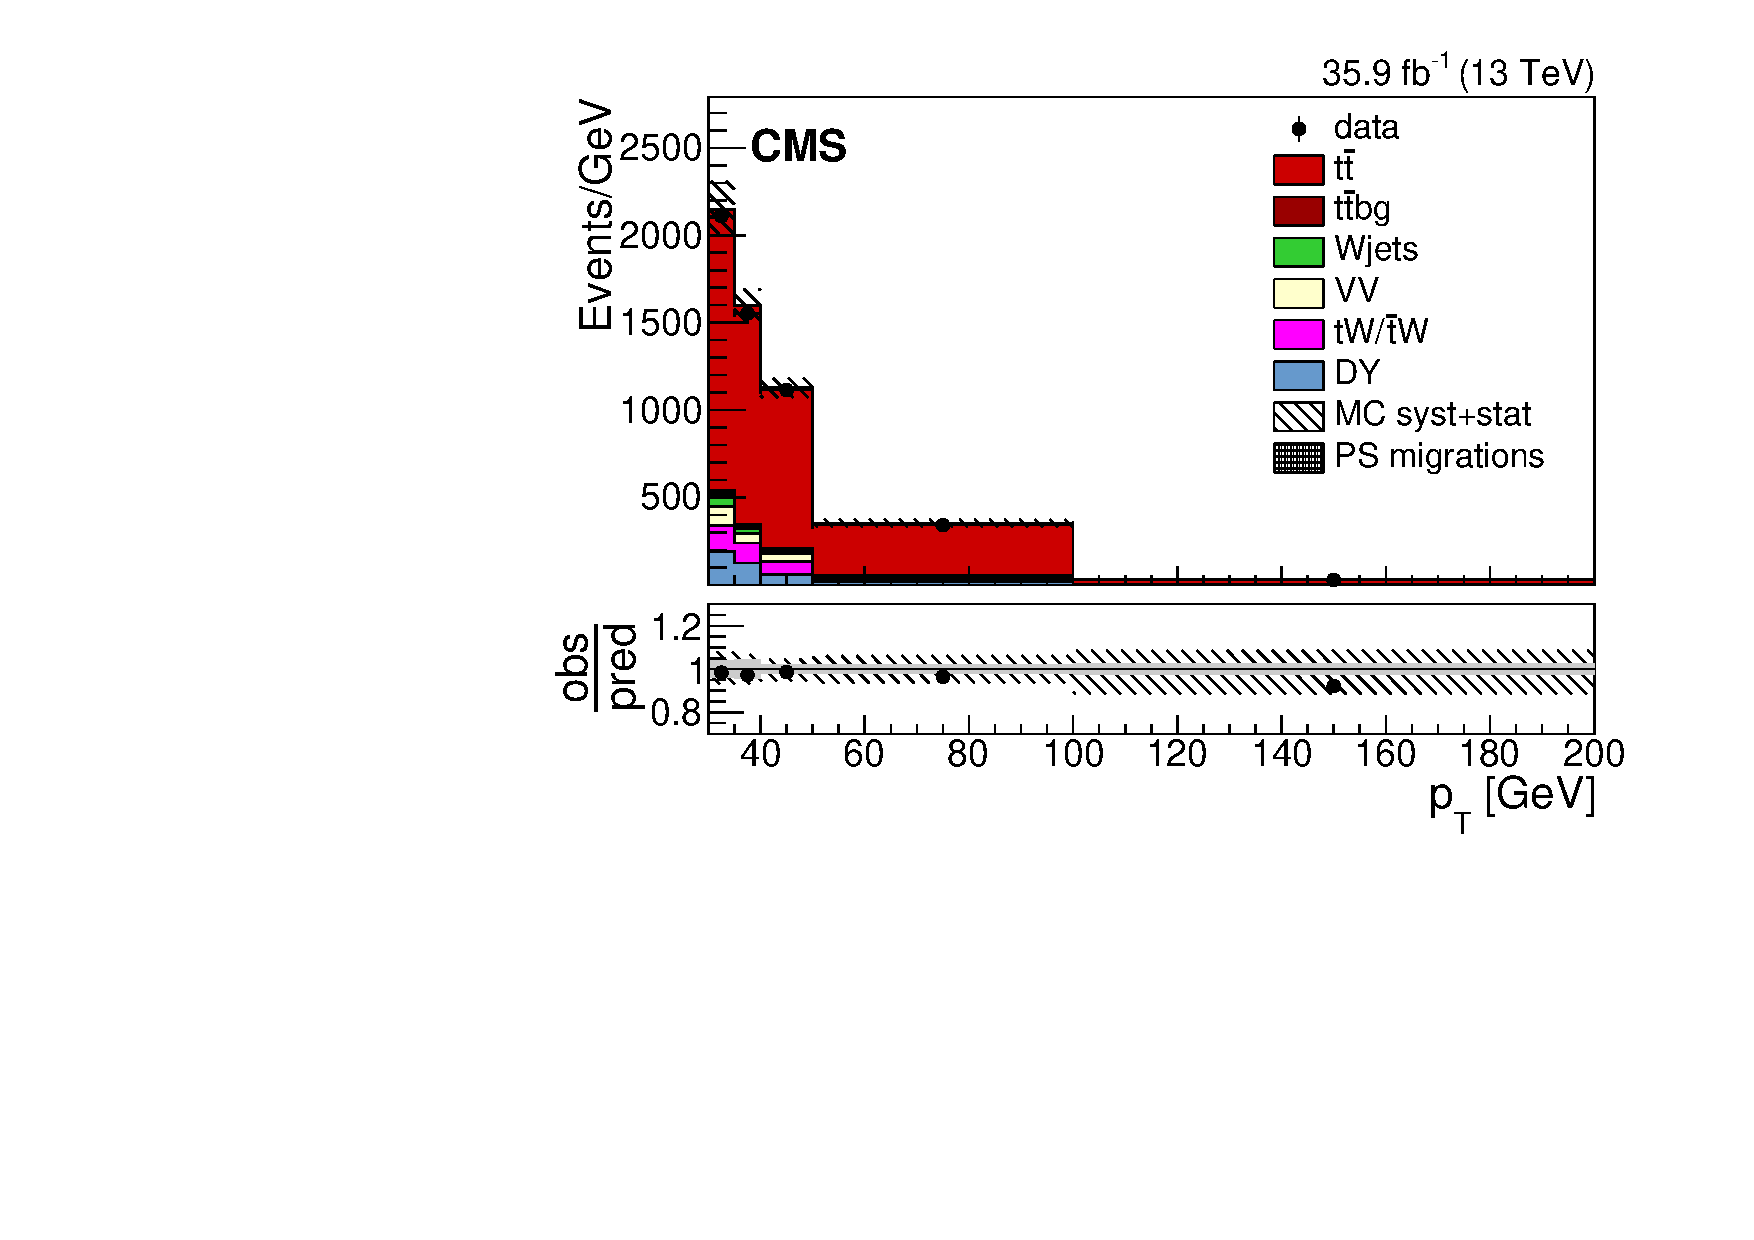
\includegraphics{CrossSection/Figures/ControlPlots/emu_sysnom/second_jet_pt_0_2_b-jets_step_8.pdf}}
    \resizebox{0.32 \textwidth}{!}{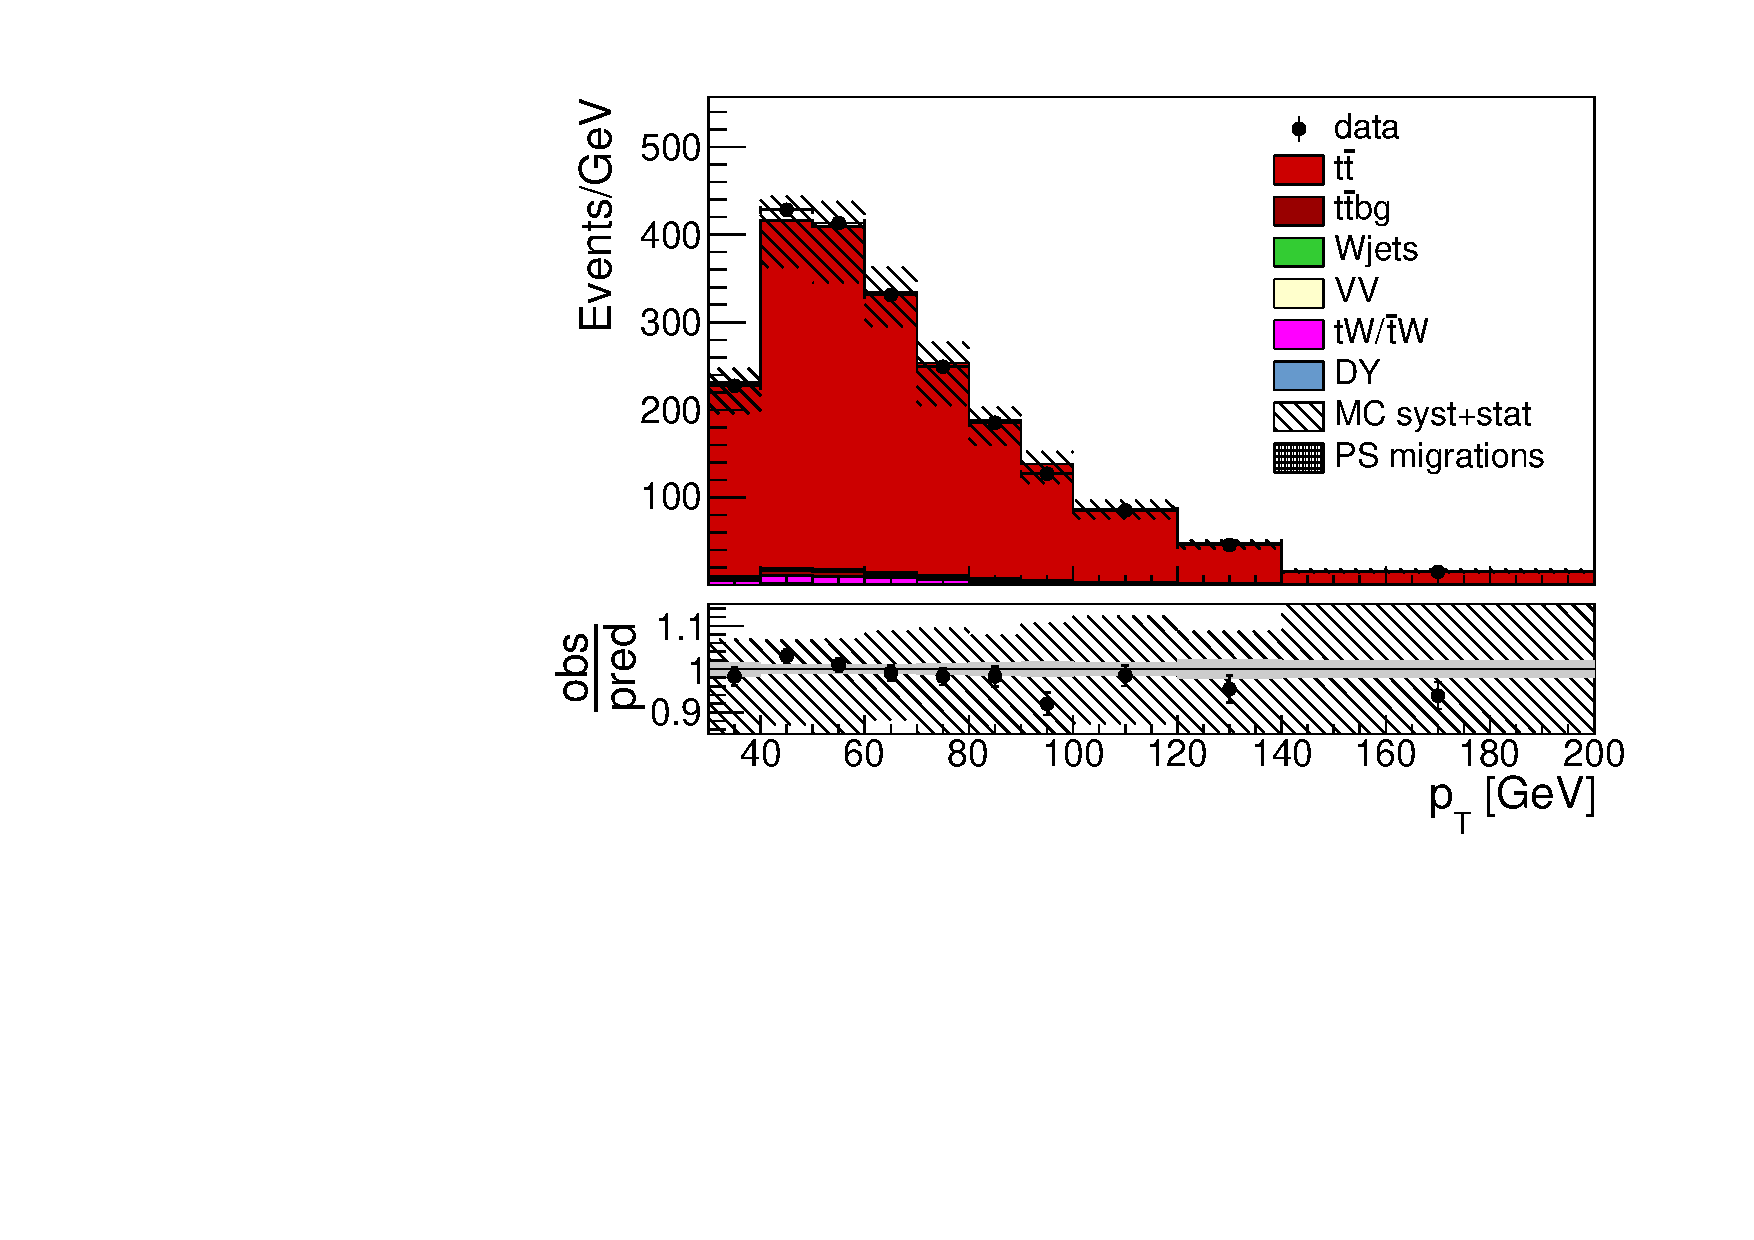
\includegraphics{CrossSection/Figures/ControlPlots/emu_sysnom/second_jet_pt_1_2_b-jets_step_8.pdf}}
    \resizebox{0.32 \textwidth}{!}{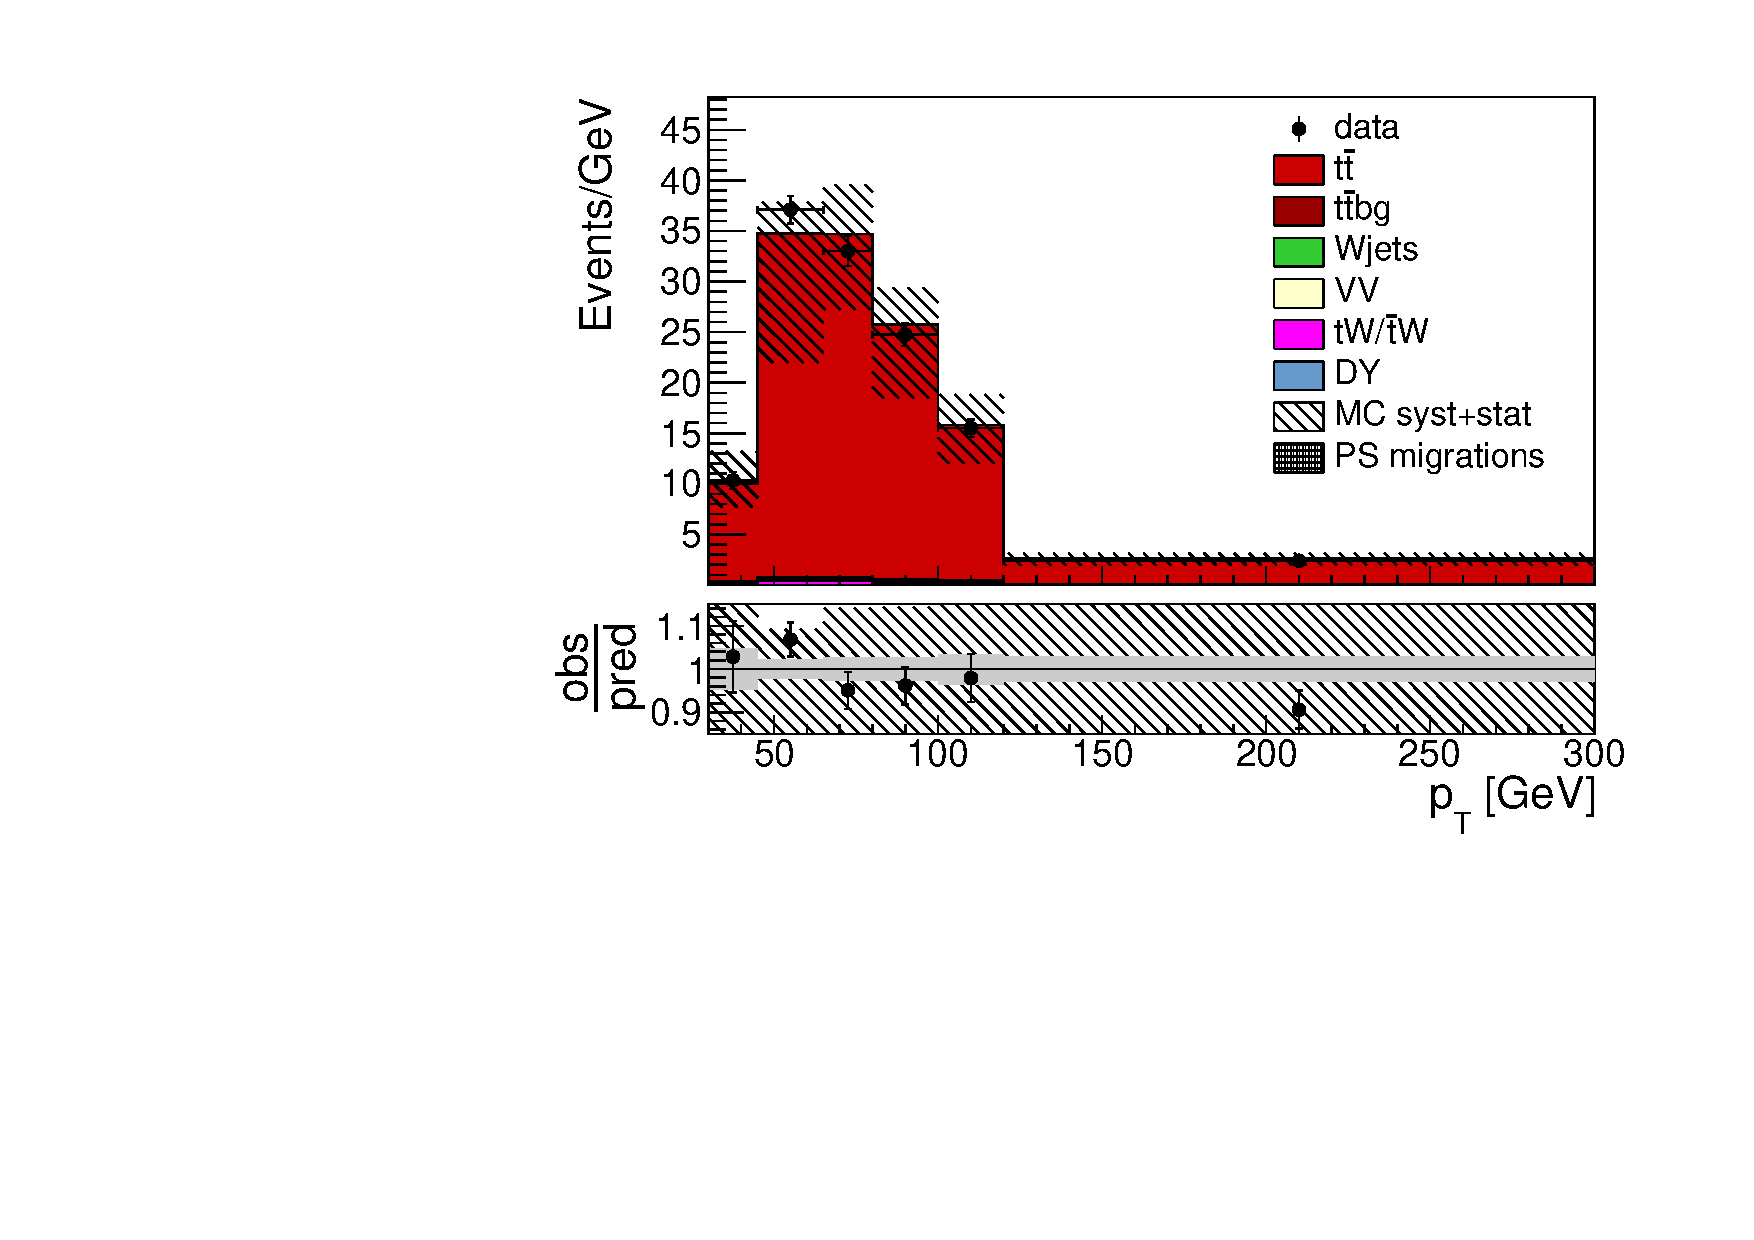
\includegraphics{CrossSection/Figures/ControlPlots/emu_sysnom/second_jet_pt_2_2_b-jets_step_8.pdf}}

    \resizebox{0.32 \textwidth}{!}{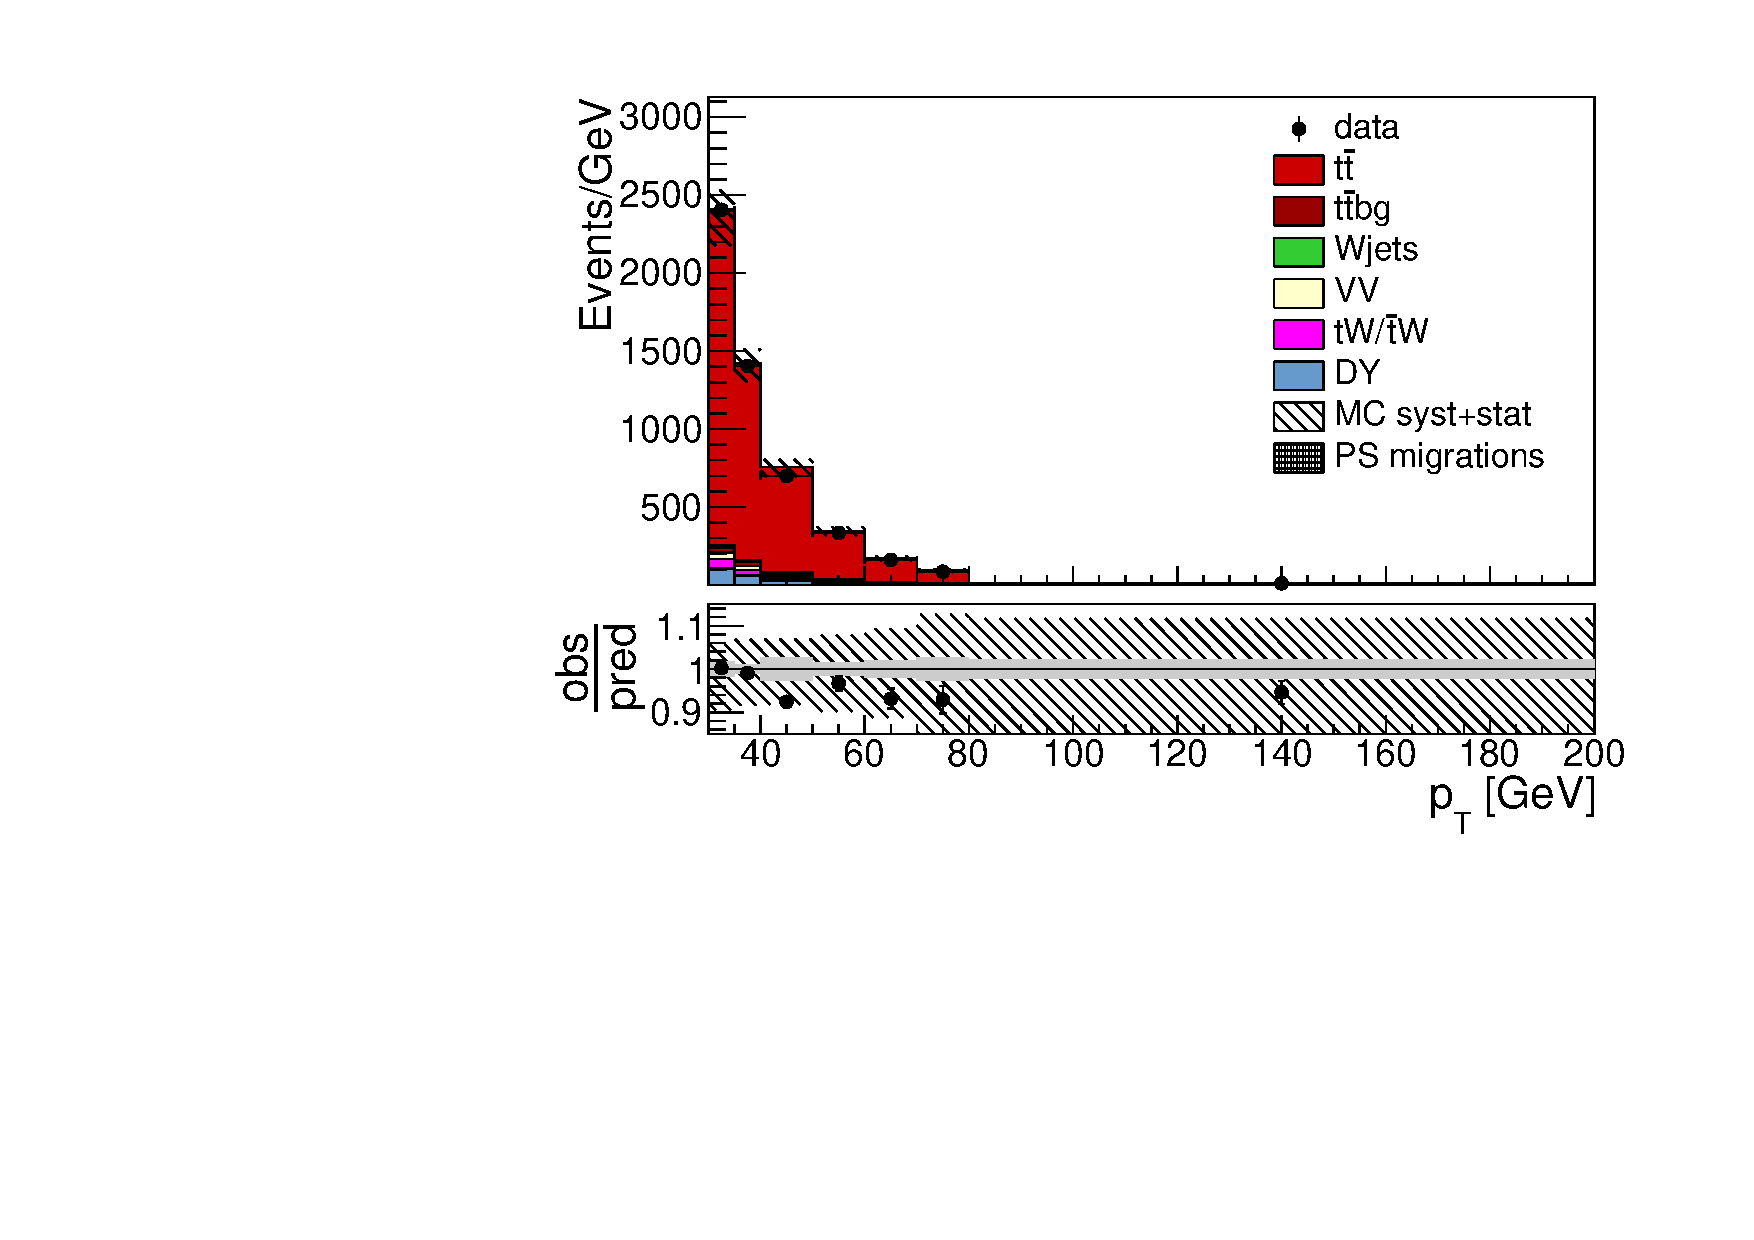
\includegraphics{CrossSection/Figures/ControlPlots/emu_sysnom/third_jet_pt_0_3_b-jets_step_8.pdf}}
    \resizebox{0.32 \textwidth}{!}{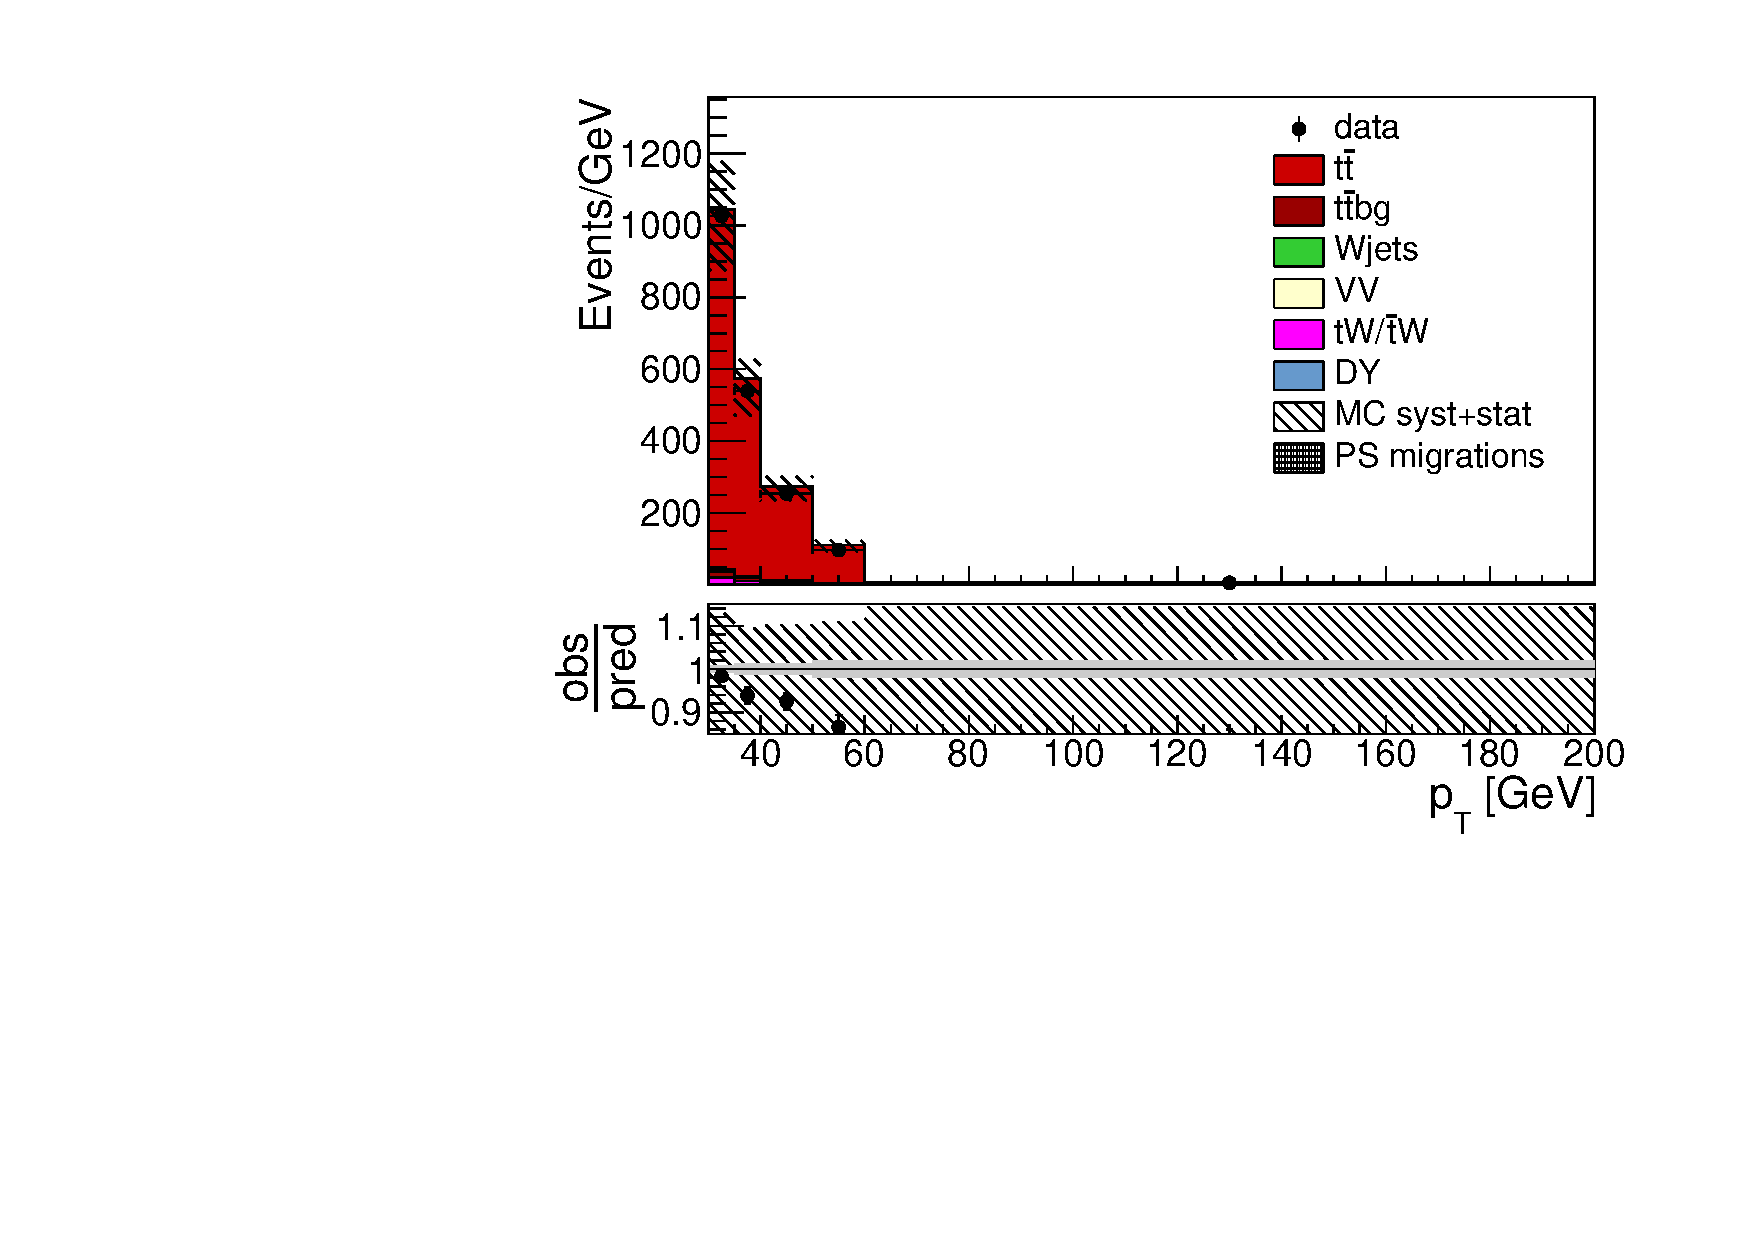
\includegraphics{CrossSection/Figures/ControlPlots/emu_sysnom/third_jet_pt_1_3_b-jets_step_8.pdf}}
    \resizebox{0.32 \textwidth}{!}{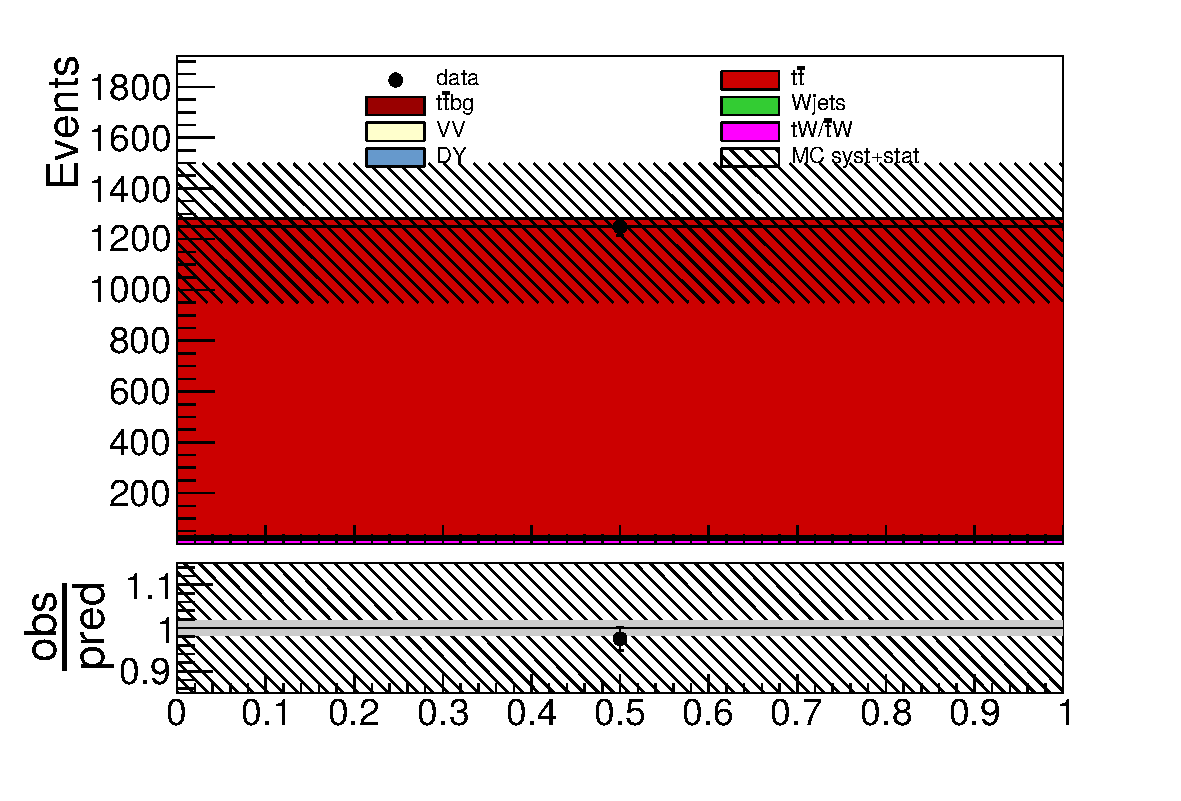
\includegraphics{CrossSection/Figures/ControlPlots/emu_sysnom/total_2_3_b-jets_step_8.pdf}}  

\caption{Template distributions for events in the \emu channel with zero as well as three or
  more b-tagged jets (left column), one b-tagged jet (middle column), or two b-tagged jets (right column). The distributions show the total event yield for zero jets (top), the \pt of the jet with the lowest \pt for one (second from top),
  two (second from bottom) or three or more (bottom) additional jets. 
  The hatched bands correspond to the total uncertainty on the predicted number of events, excluding luminosity and background
        normalization uncertainties.  The ratios of the event yields in data and the sum of the
  predicted yields are shown at the bottom of each figure. Here, the solid
  gray band represents the contribution of the statistical uncertainty.  
       \label{fig:xsec_emu_inputdistr}}
  \end{center}
\end{figure}

\begin{figure}[htbp!]
  \begin{center}
    \resizebox{0.40 \textwidth}{!}{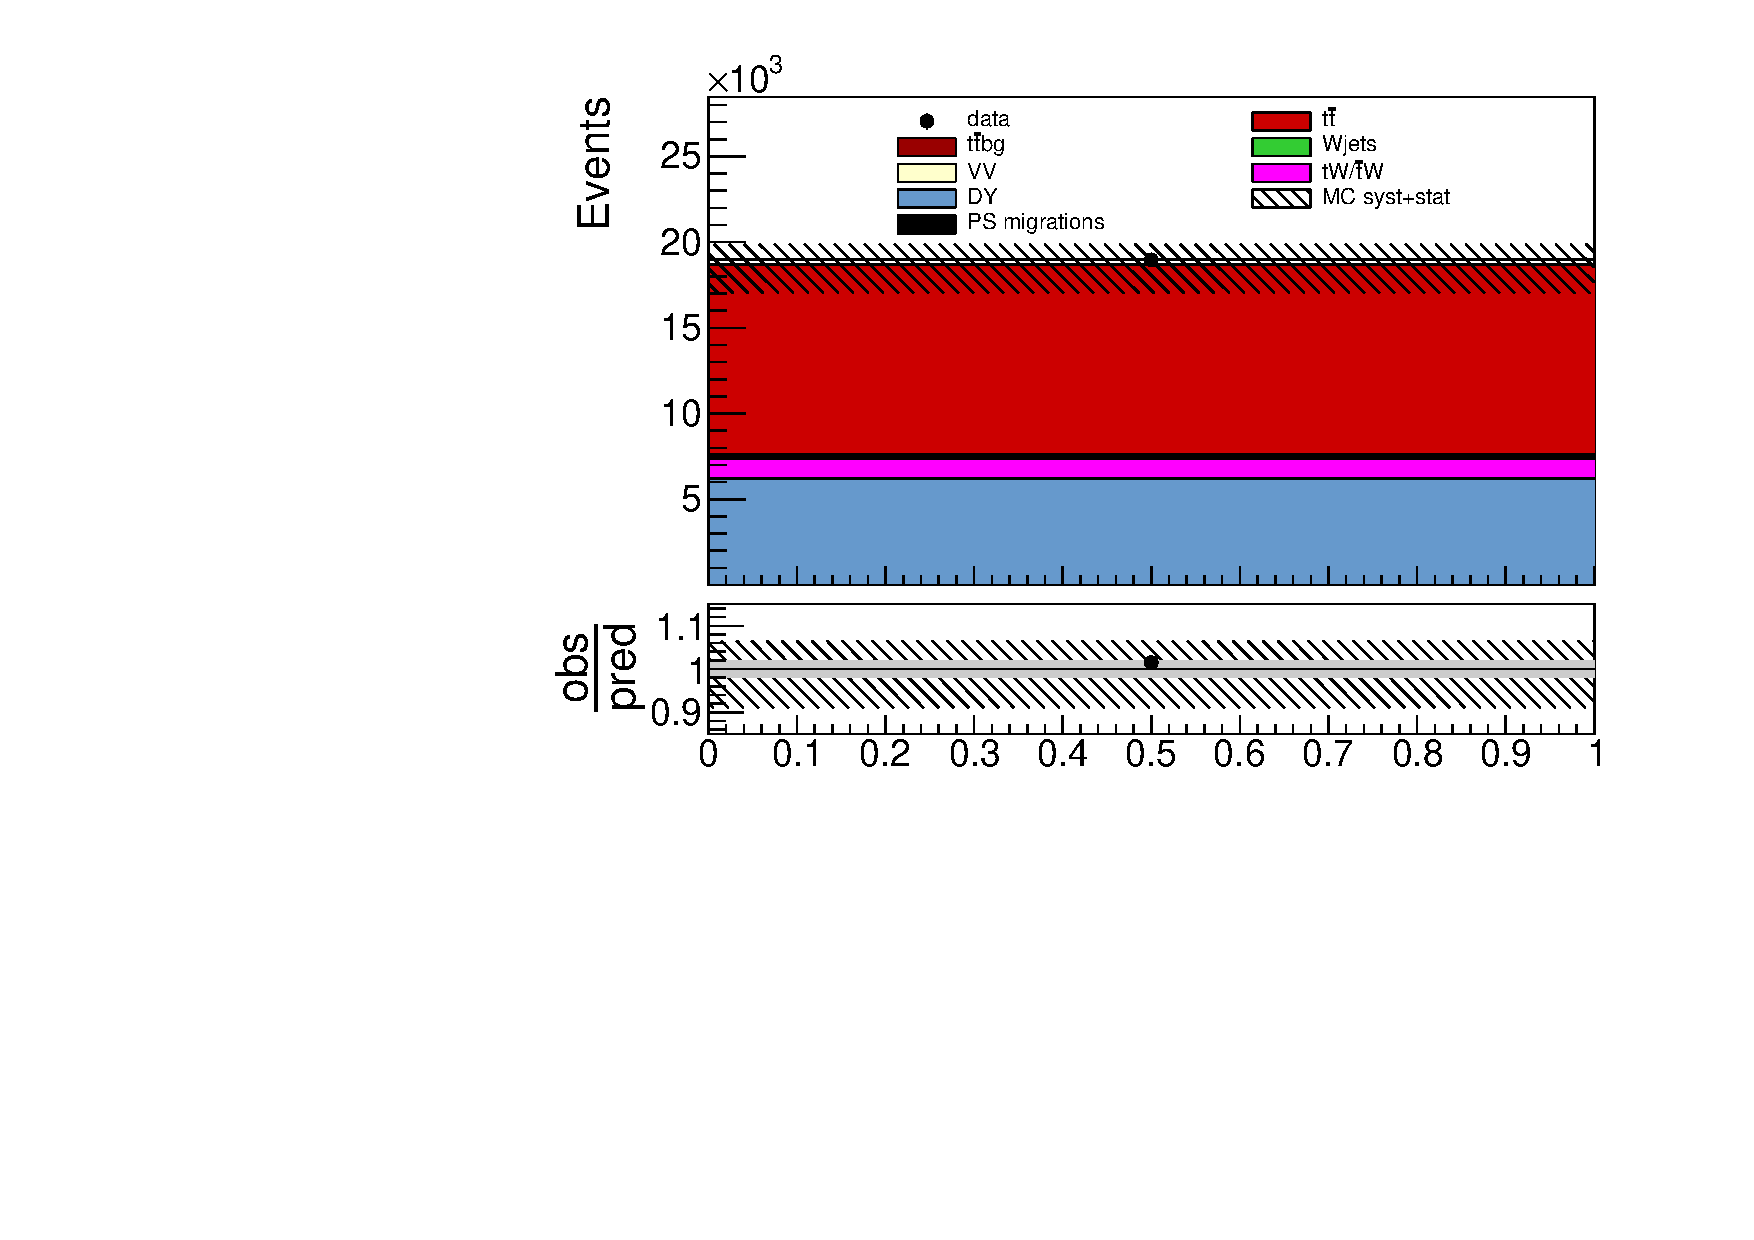
\includegraphics{CrossSection/Figures/ControlPlots/mumu_sysnom/total_1_0_b-jets_step_8.pdf}}
    \resizebox{0.40 \textwidth}{!}{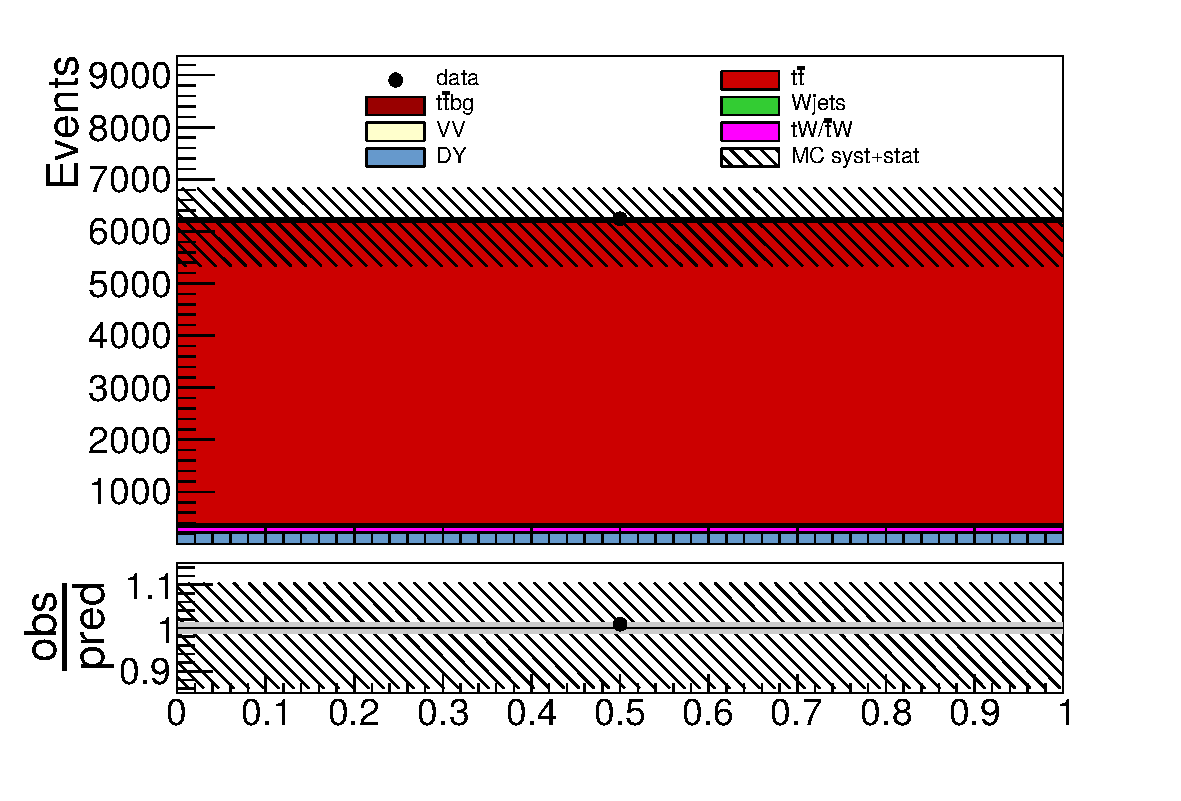
\includegraphics{CrossSection/Figures/ControlPlots/mumu_sysnom/total_2_0_b-jets_step_8.pdf}} \\

    \resizebox{0.40 \textwidth}{!}{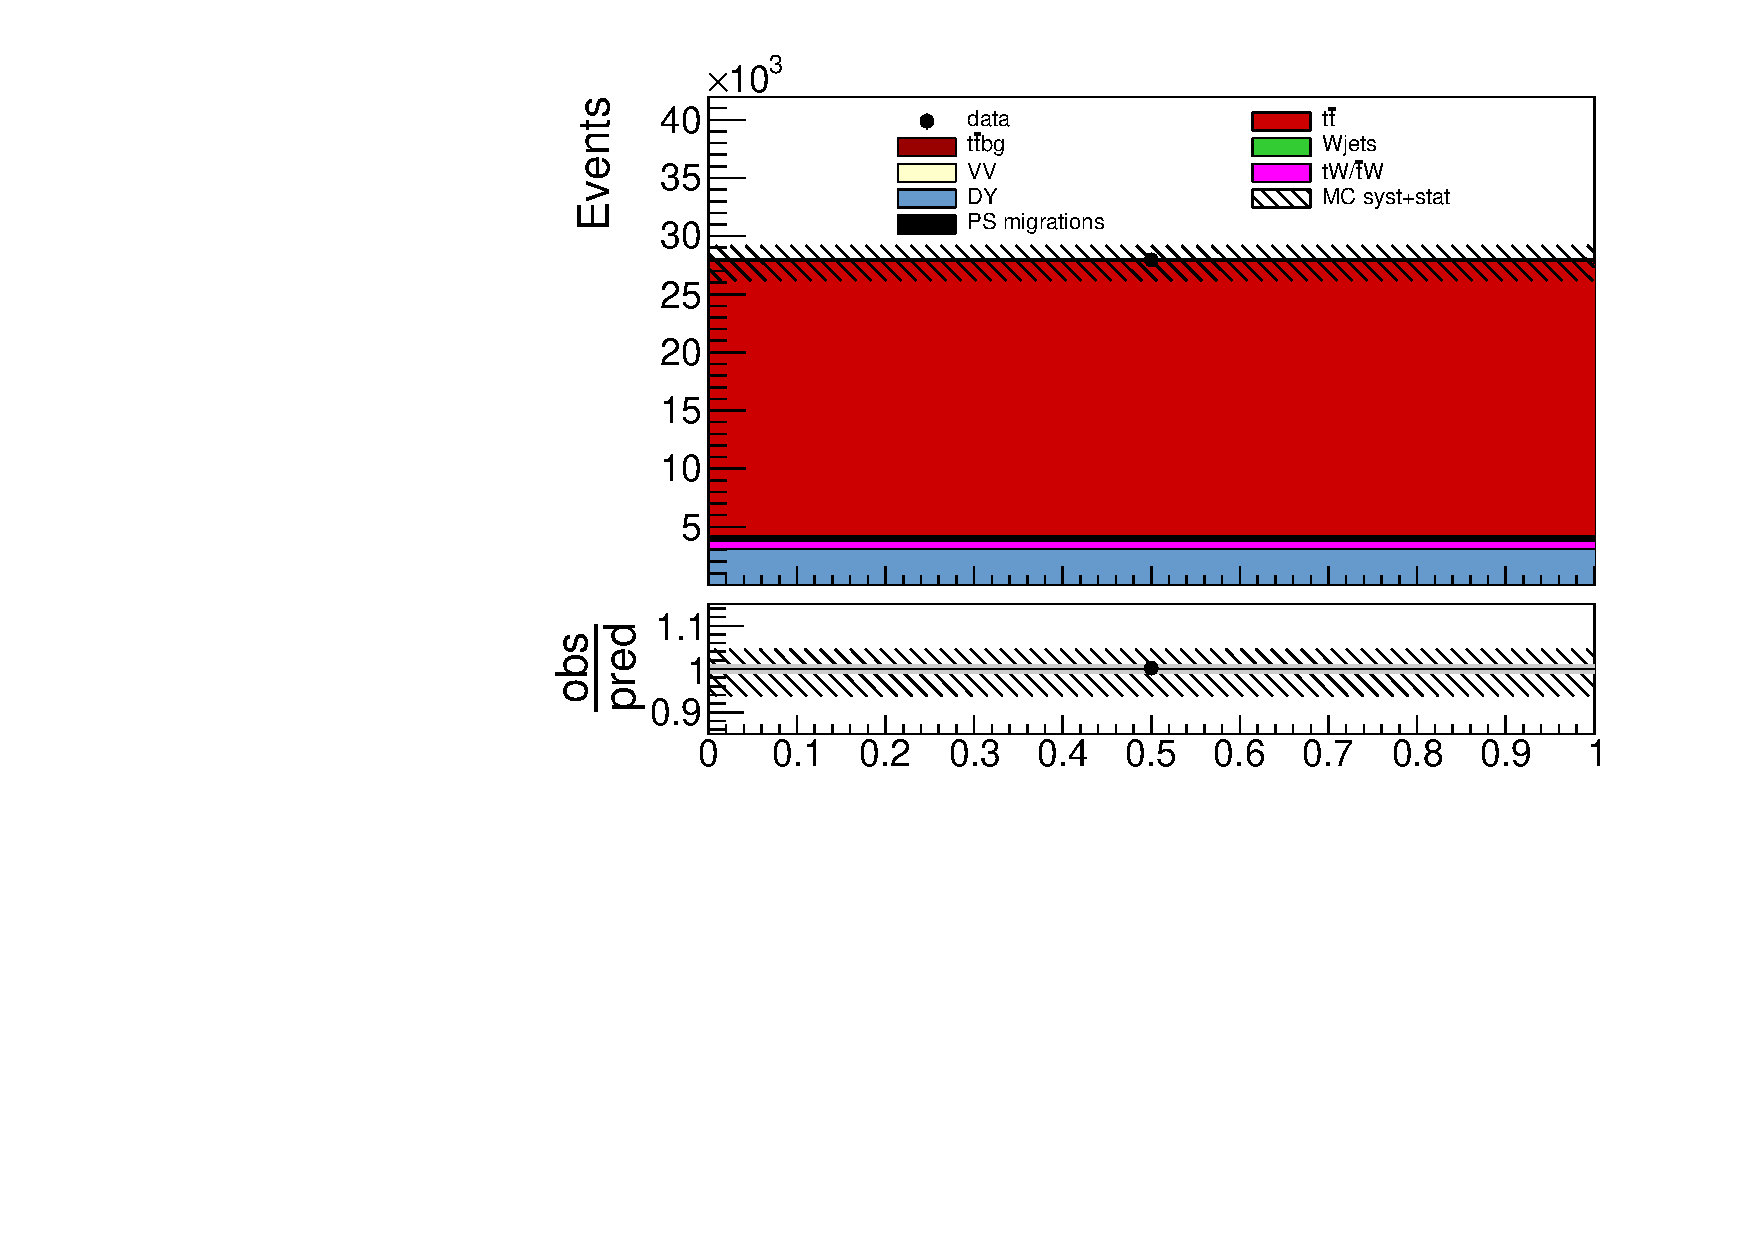
\includegraphics{CrossSection/Figures/ControlPlots/mumu_sysnom/total_1_1_b-jets_step_8.pdf}}
    \resizebox{0.40 \textwidth}{!}{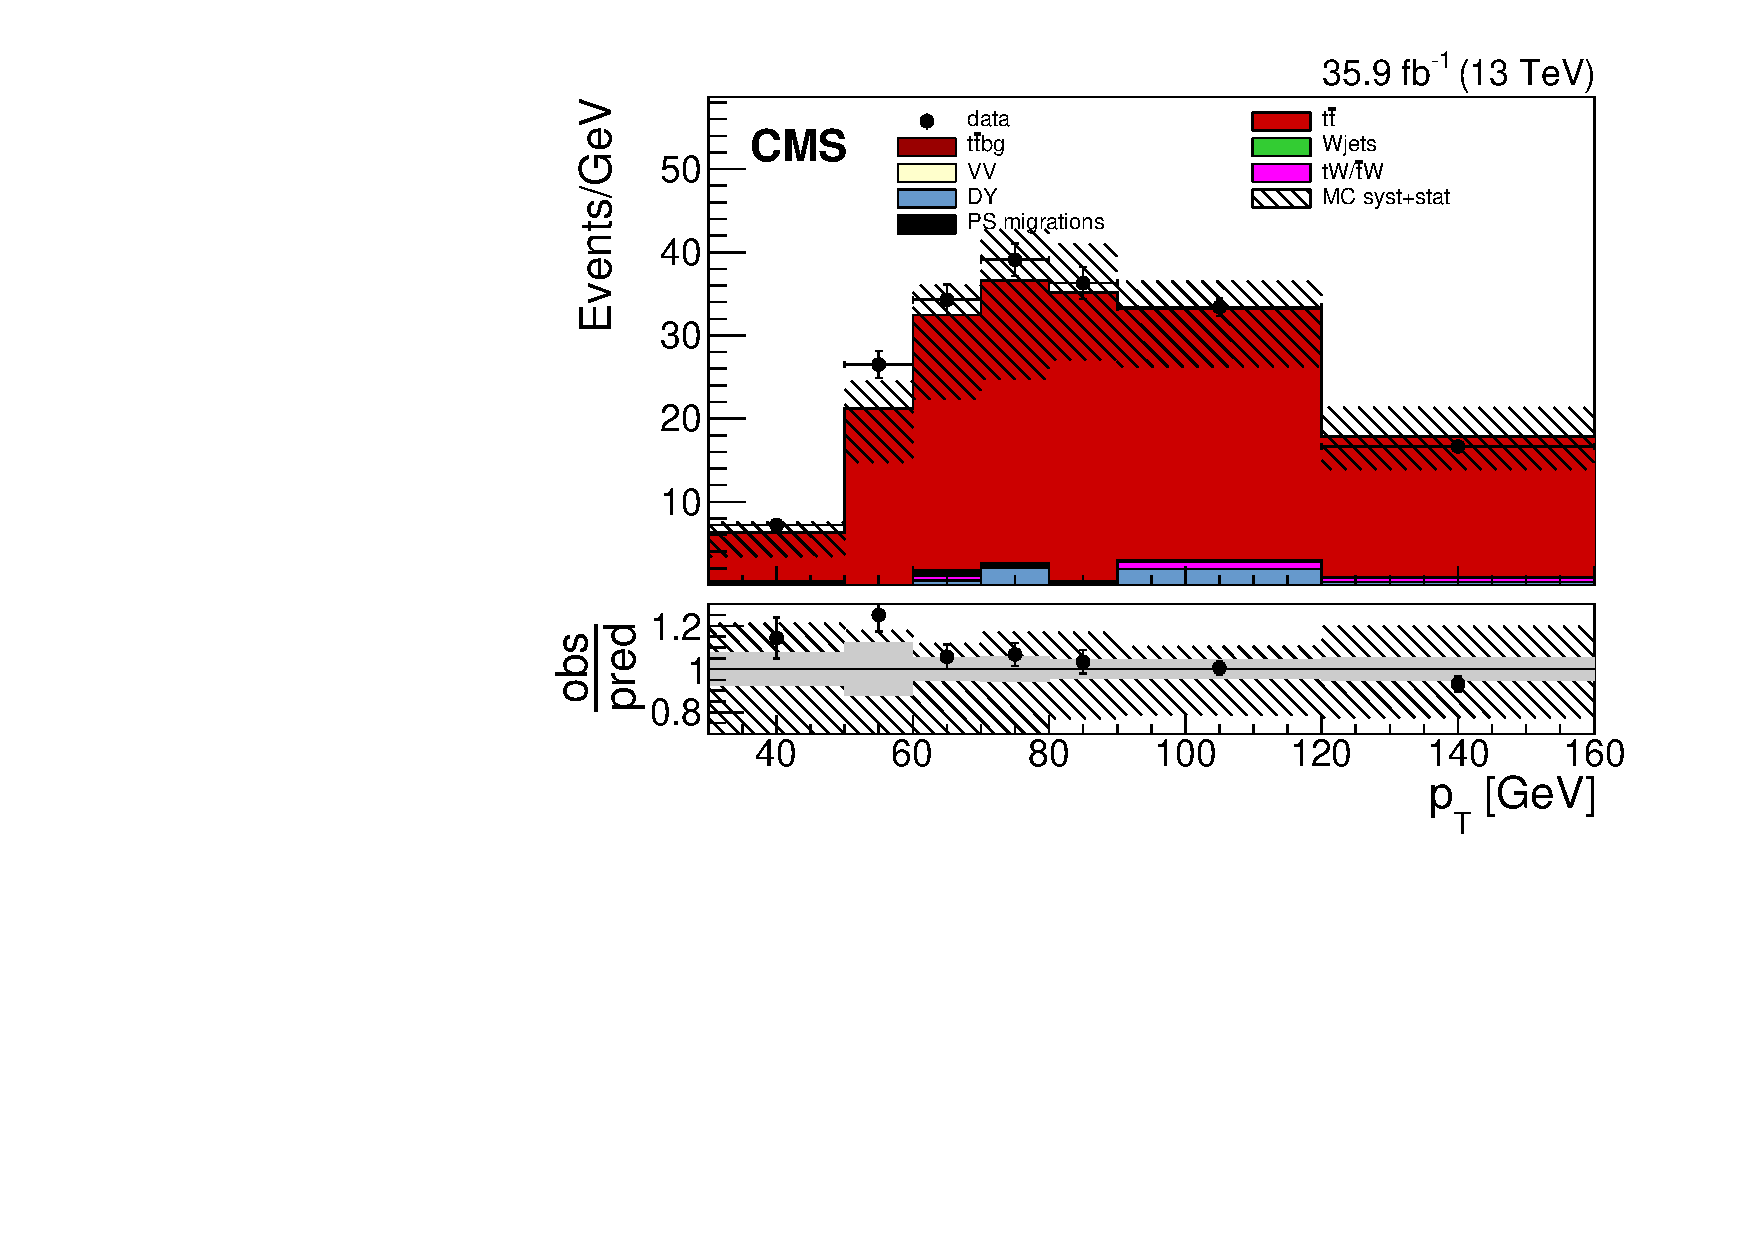
\includegraphics{CrossSection/Figures/ControlPlots/mumu_sysnom/lead_jet_pt_2_1_b-jets_step_8.pdf}}\\
        
    \resizebox{0.4 \textwidth}{!}{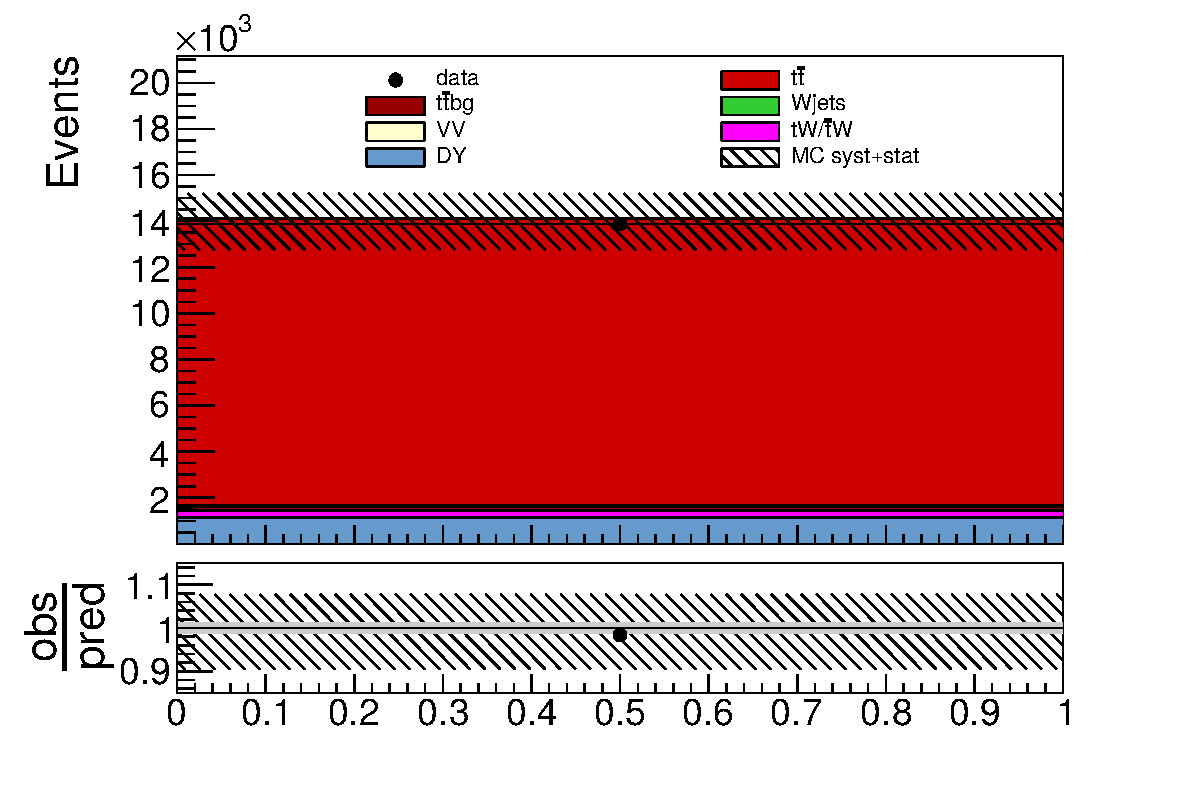
\includegraphics{CrossSection/Figures/ControlPlots/mumu_sysnom/total_1_2_b-jets_step_8.pdf}}
    \resizebox{0.4 \textwidth}{!}{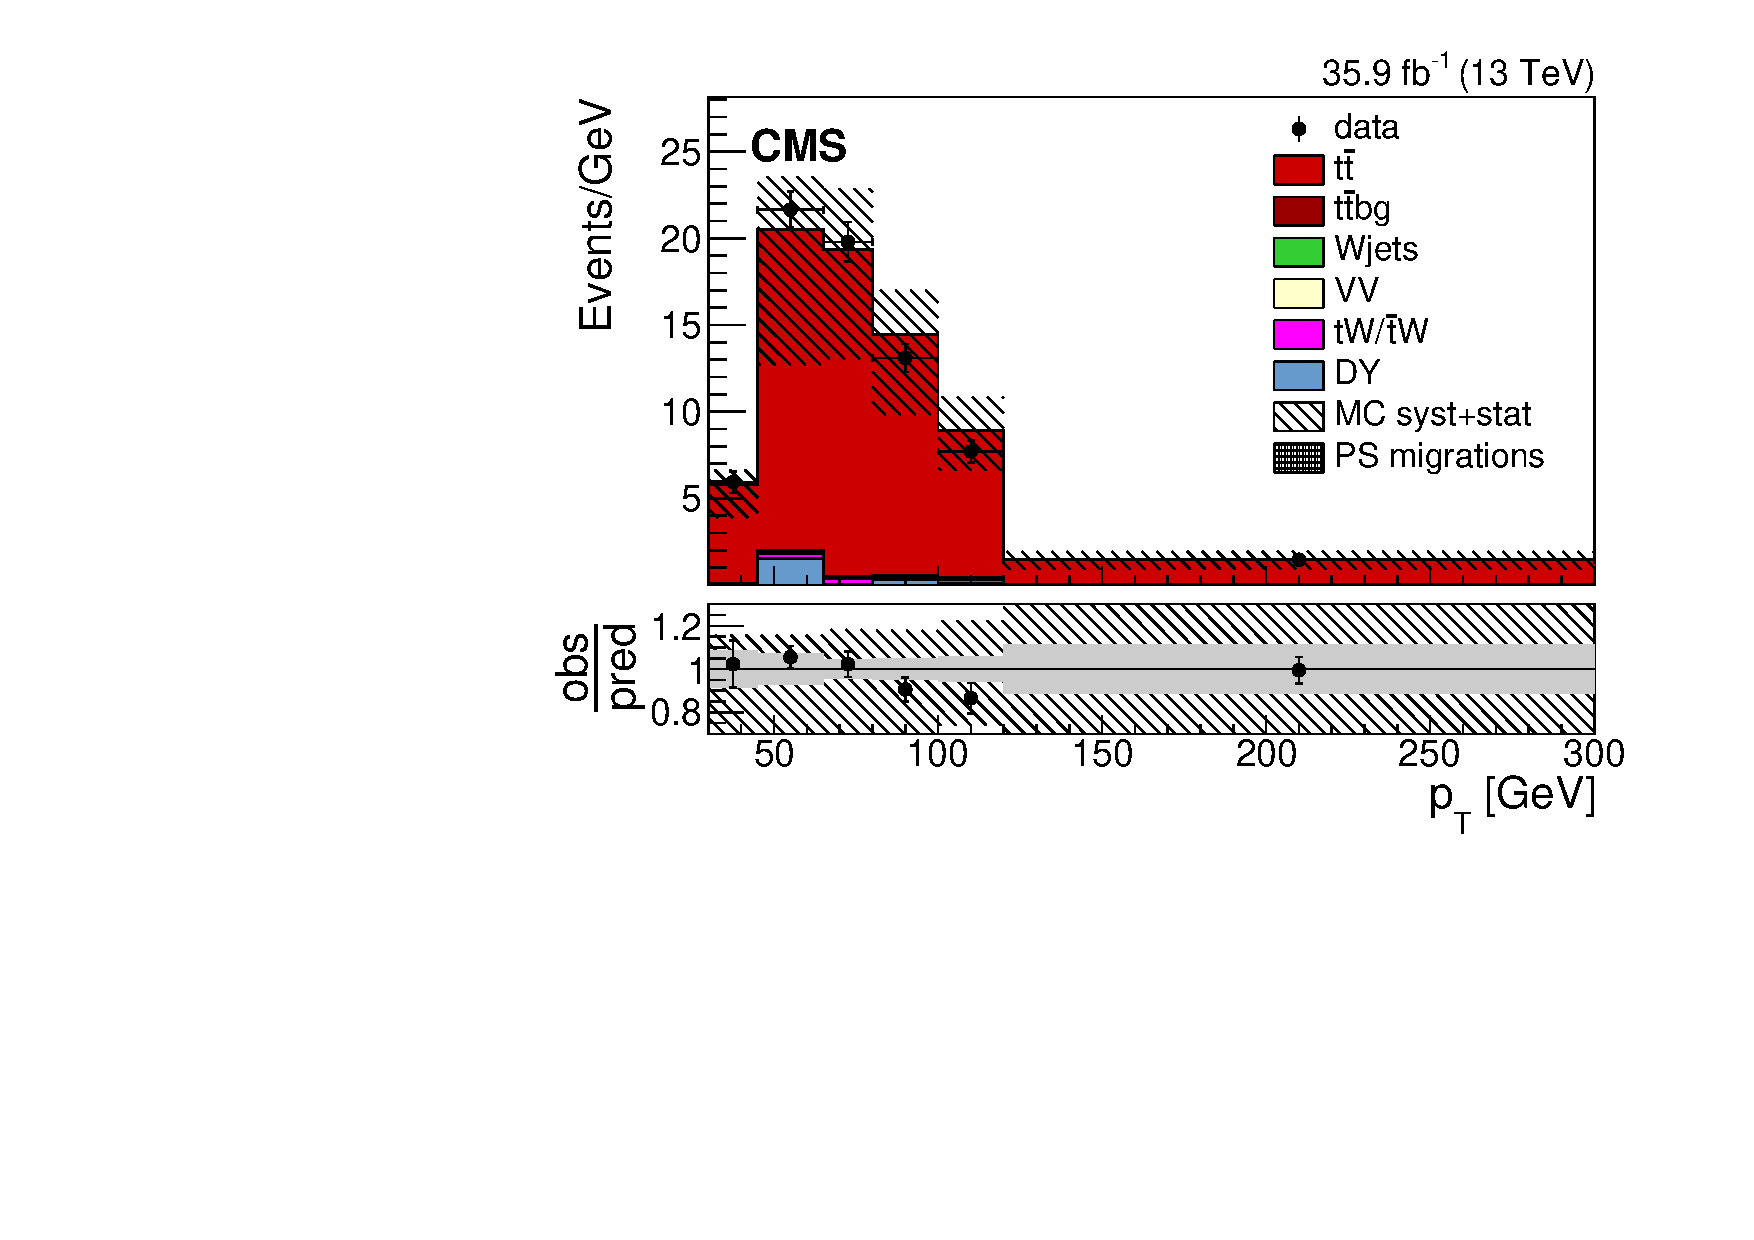
\includegraphics{CrossSection/Figures/ControlPlots/mumu_sysnom/second_jet_pt_2_2_b-jets_step_8.pdf}}\\

    \resizebox{0.4 \textwidth}{!}{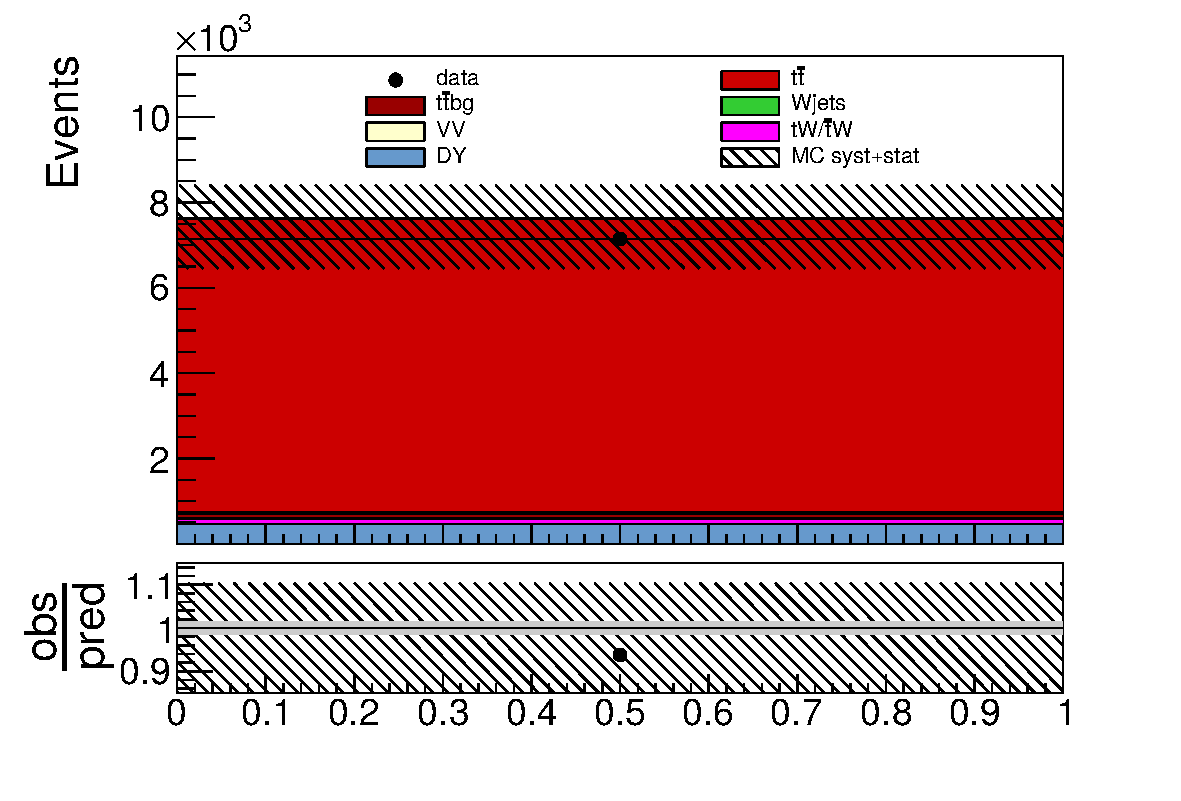
\includegraphics{CrossSection/Figures/ControlPlots/mumu_sysnom/total_1_3_b-jets_step_8.pdf}}
    \resizebox{0.4 \textwidth}{!}{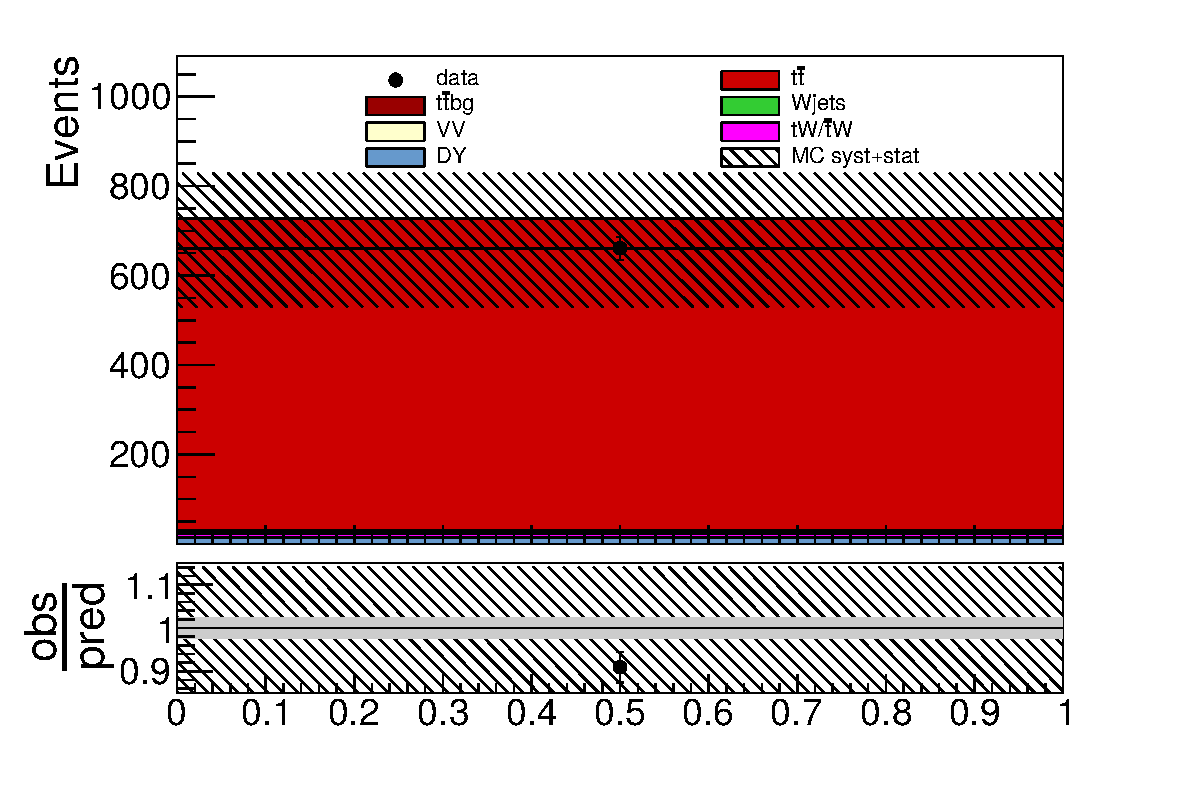
\includegraphics{CrossSection/Figures/ControlPlots/mumu_sysnom/total_2_3_b-jets_step_8.pdf}}  
\caption{Template distributions for events in the \mumu channel with one b-tagged jet (left column) or two b-tagged jets (right column). The distributions show the total event yield for zero (top), the \pt of the jet with the lowest \pt  for one (second from top),
  two (second from bottom) or three or more (bottom) additional jets. 
  The hatched bands correspond to the total uncertainty on the predicted number of events, excluding luminosity and background
        normalization uncertainties.  The ratios of the event yields in data and the sum of the
  predicted yields are shown at the bottom of each plot. Here, the solid
  gray band represents the contribution of the statistical uncertainty.  
       \label{fig:xsec_mumu_inputdistr}}
  \end{center}
\end{figure}

\begin{figure}[htbp!]
  \begin{center}
    \resizebox{0.4 \textwidth}{!}{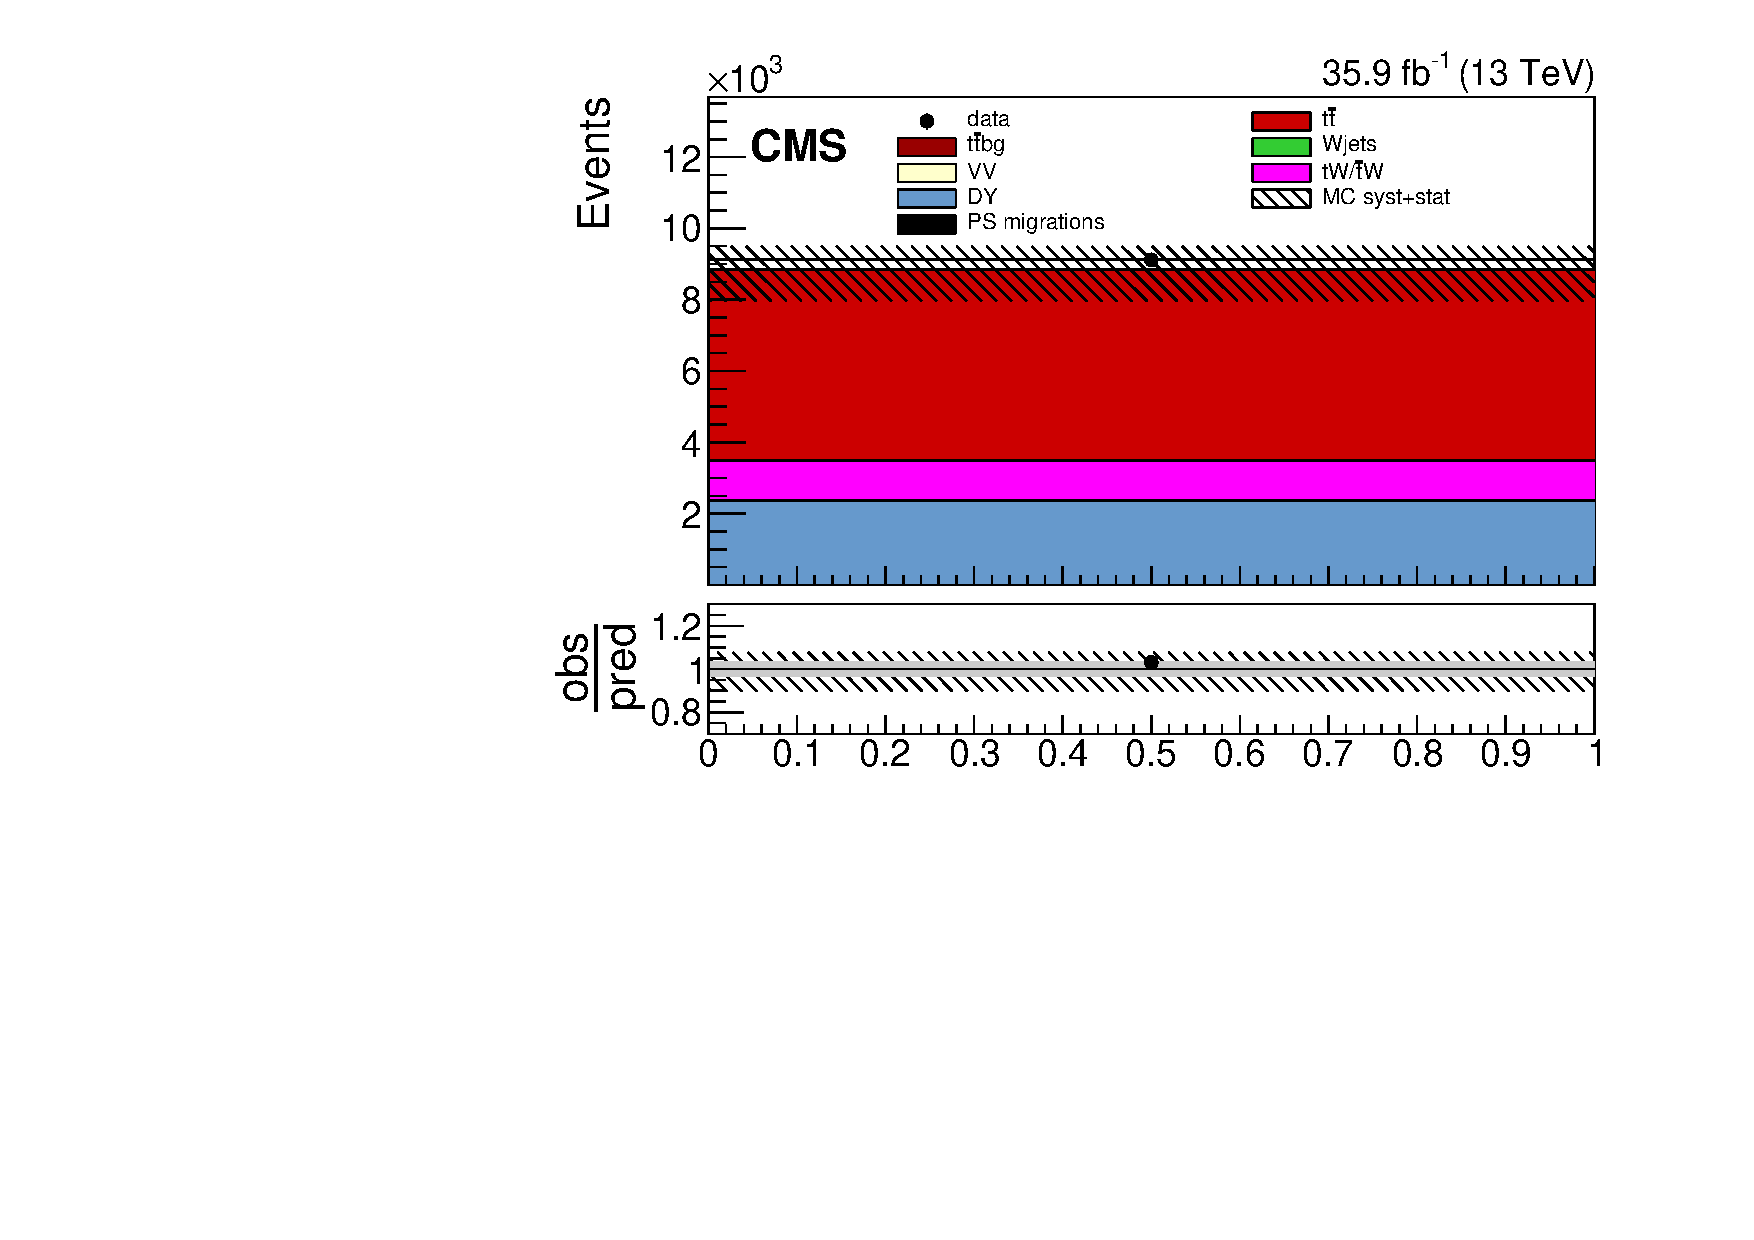
\includegraphics{CrossSection/Figures/ControlPlots/ee_sysnom/total_1_0_b-jets_step_8.pdf}}
    \resizebox{0.4 \textwidth}{!}{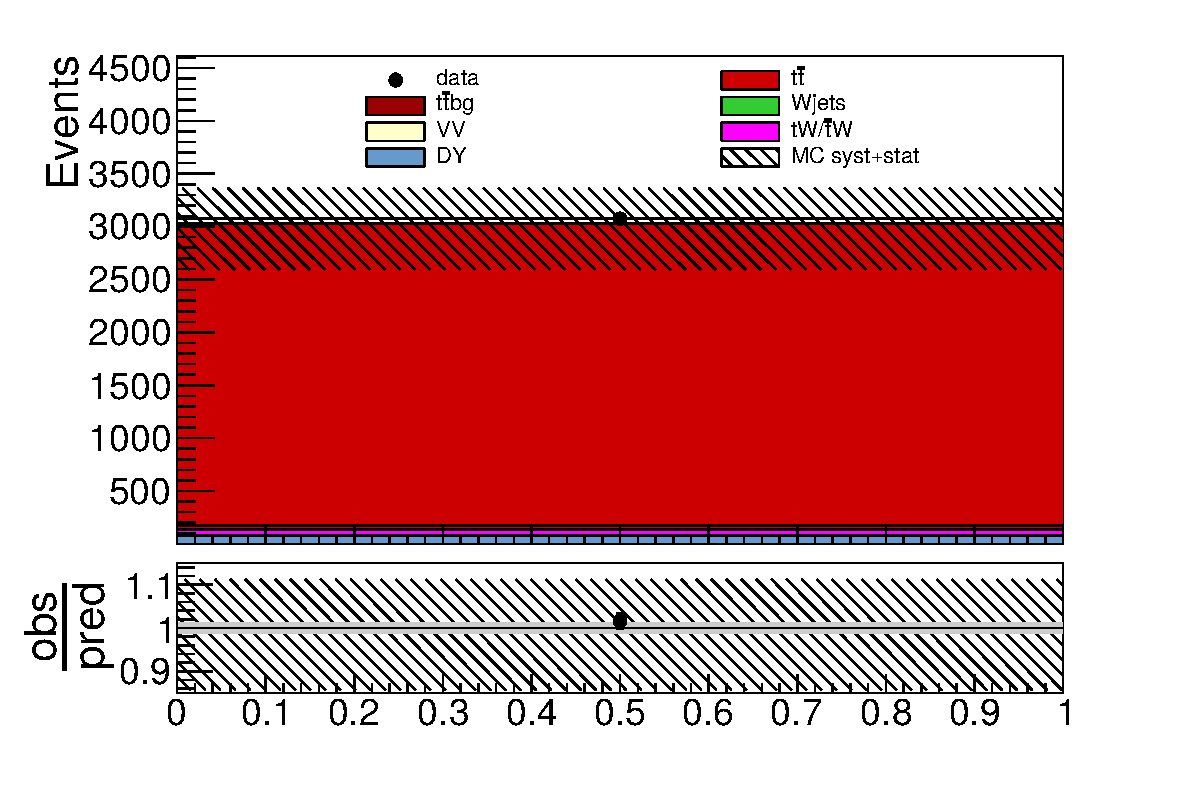
\includegraphics{CrossSection/Figures/ControlPlots/ee_sysnom/total_2_0_b-jets_step_8.pdf}}\\

    \resizebox{0.4 \textwidth}{!}{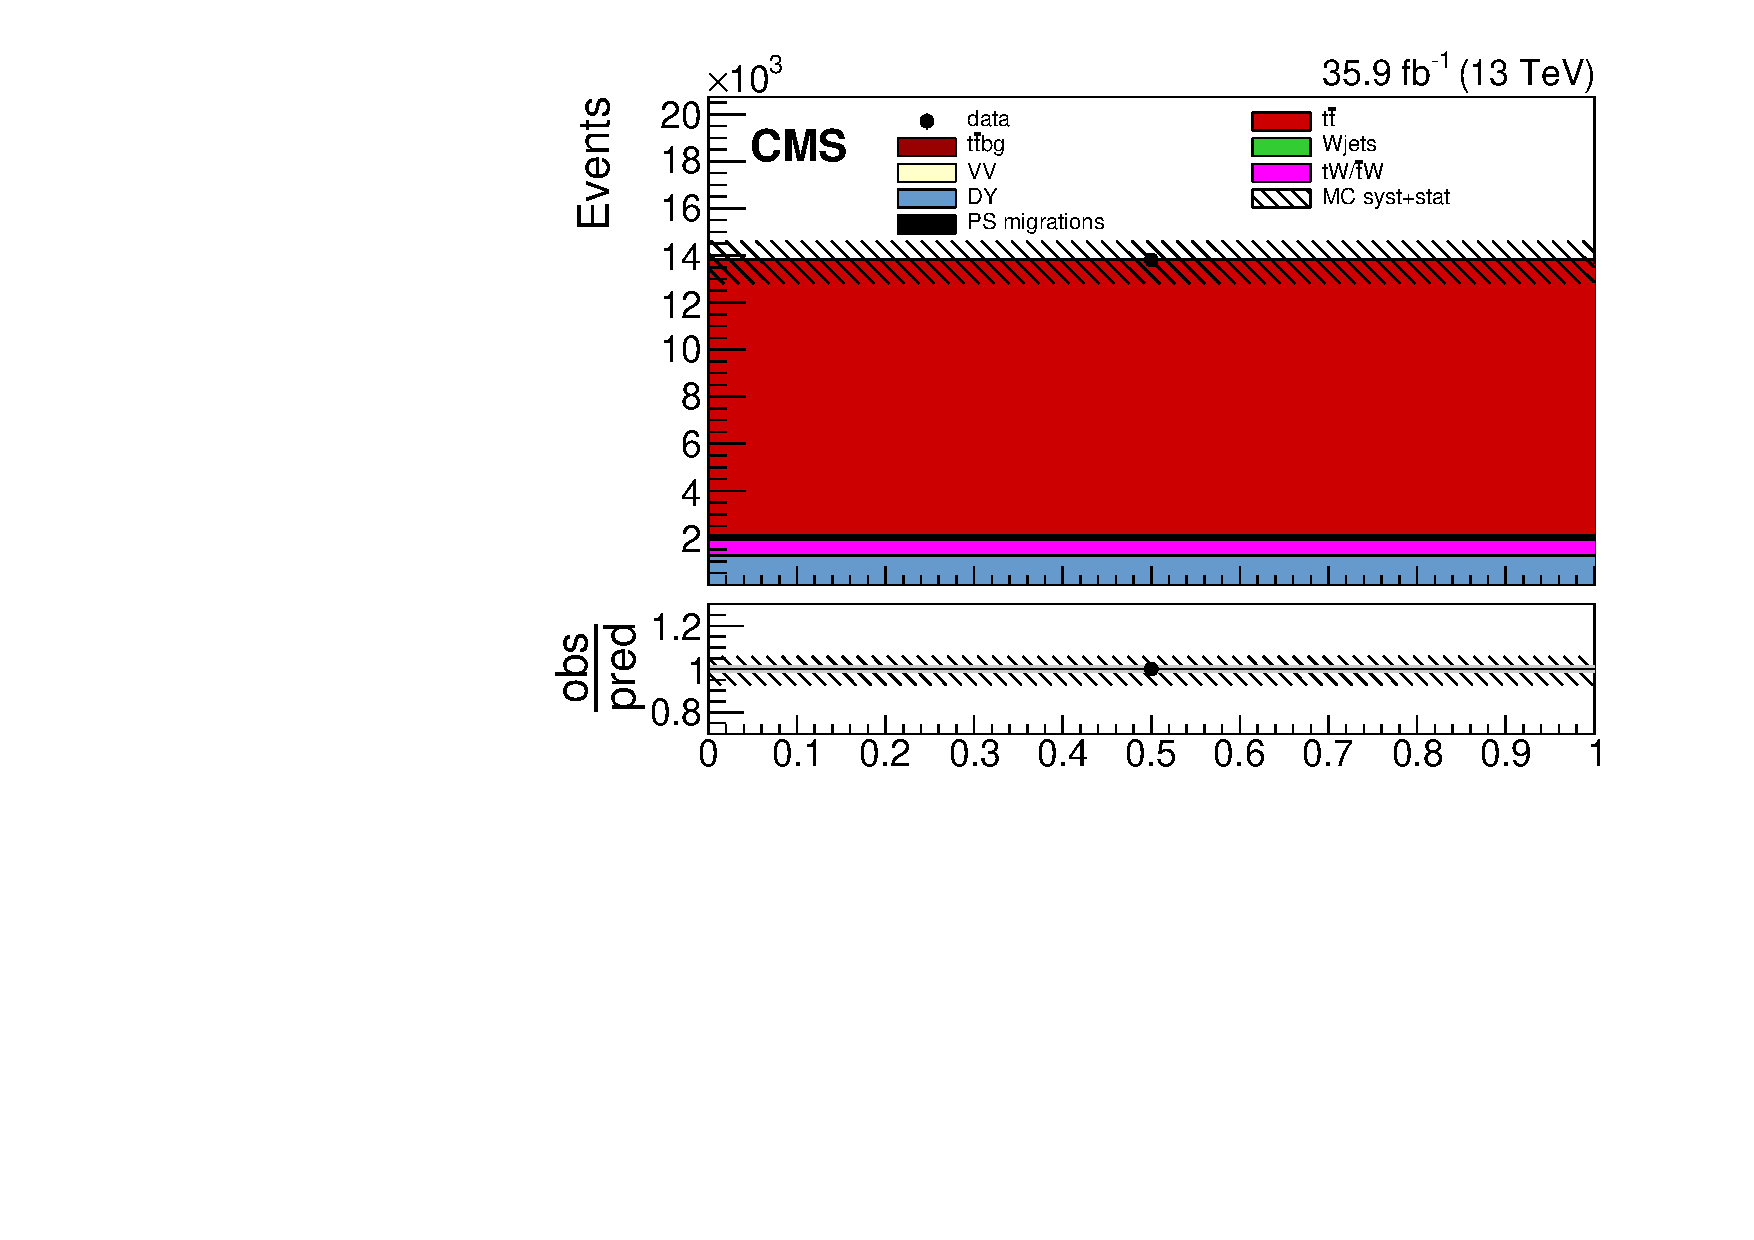
\includegraphics{CrossSection/Figures/ControlPlots/ee_sysnom/total_1_1_b-jets_step_8.pdf}}
    \resizebox{0.4 \textwidth}{!}{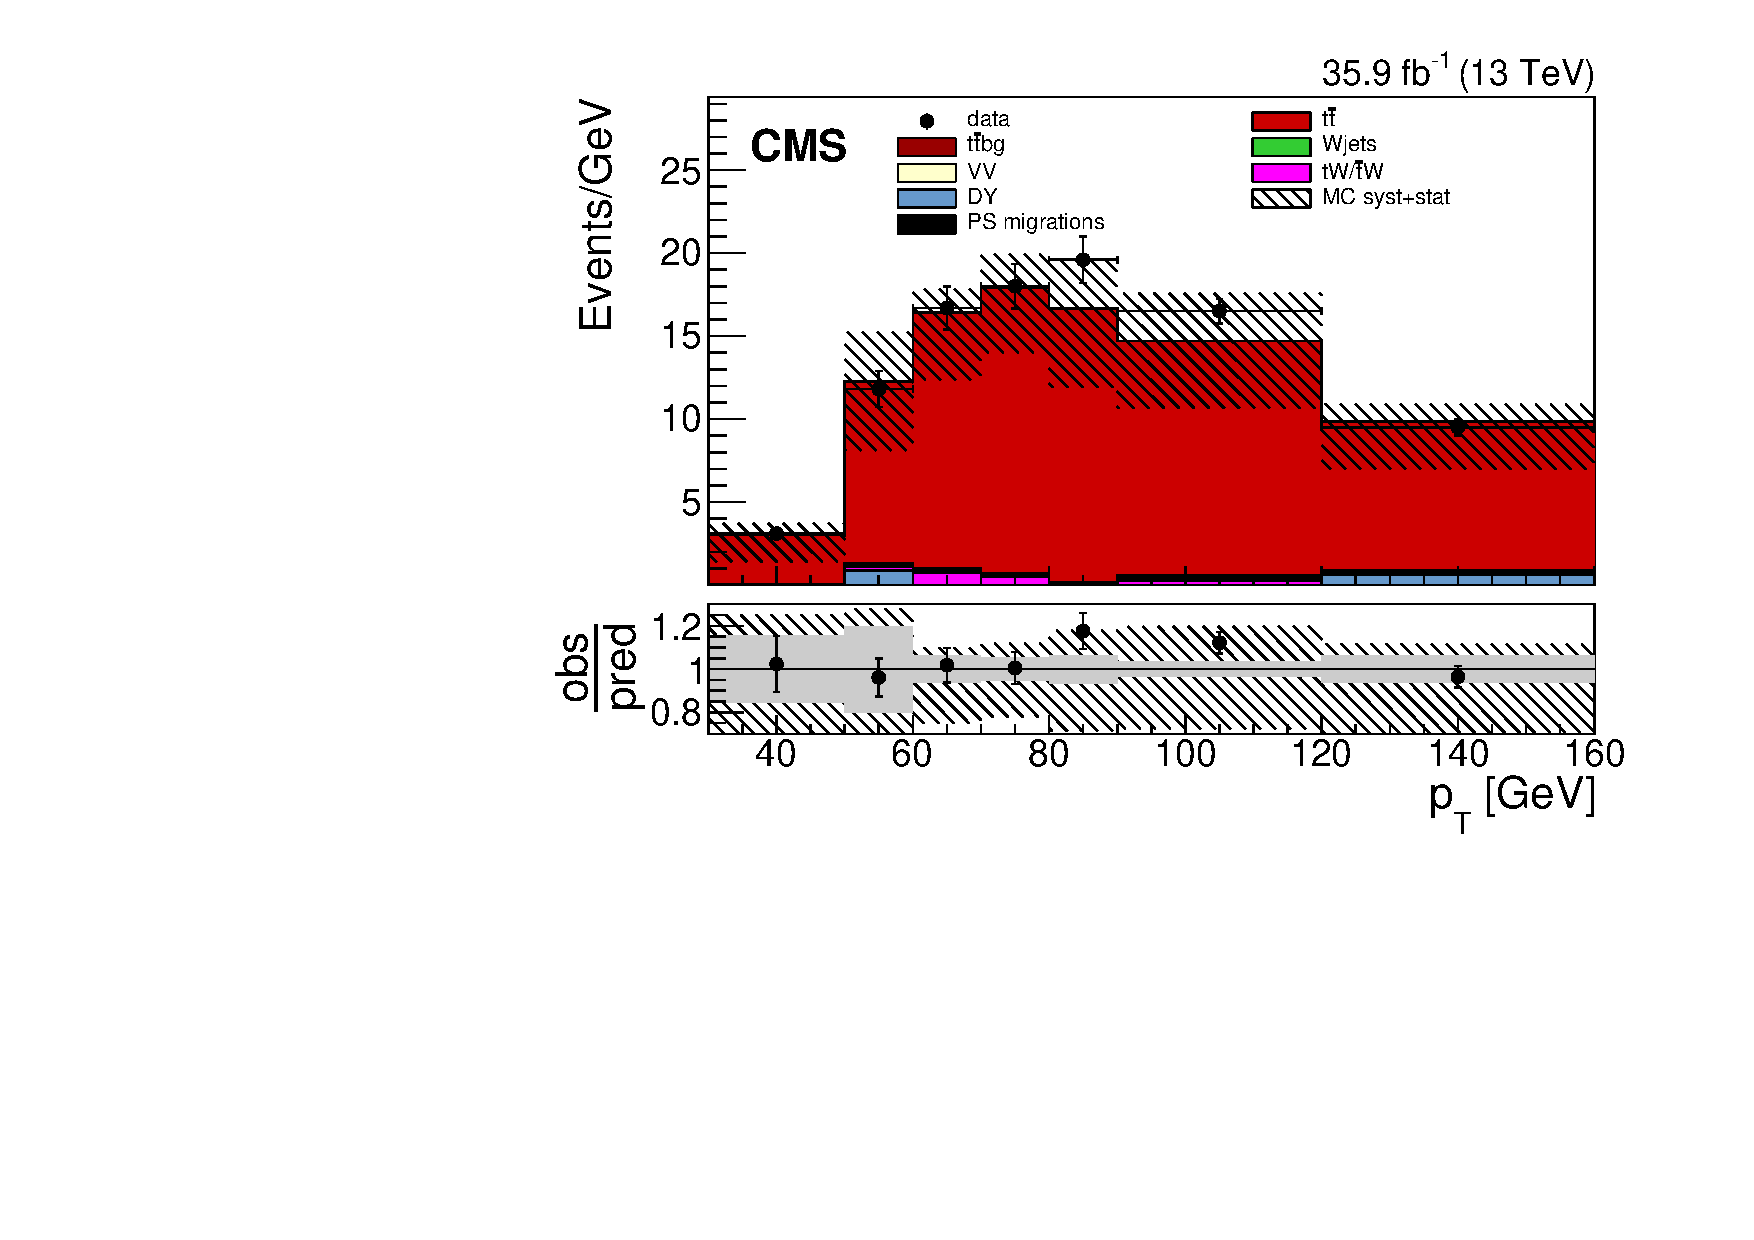
\includegraphics{CrossSection/Figures/ControlPlots/ee_sysnom/lead_jet_pt_2_1_b-jets_step_8.pdf}}\\
        
    \resizebox{0.4 \textwidth}{!}{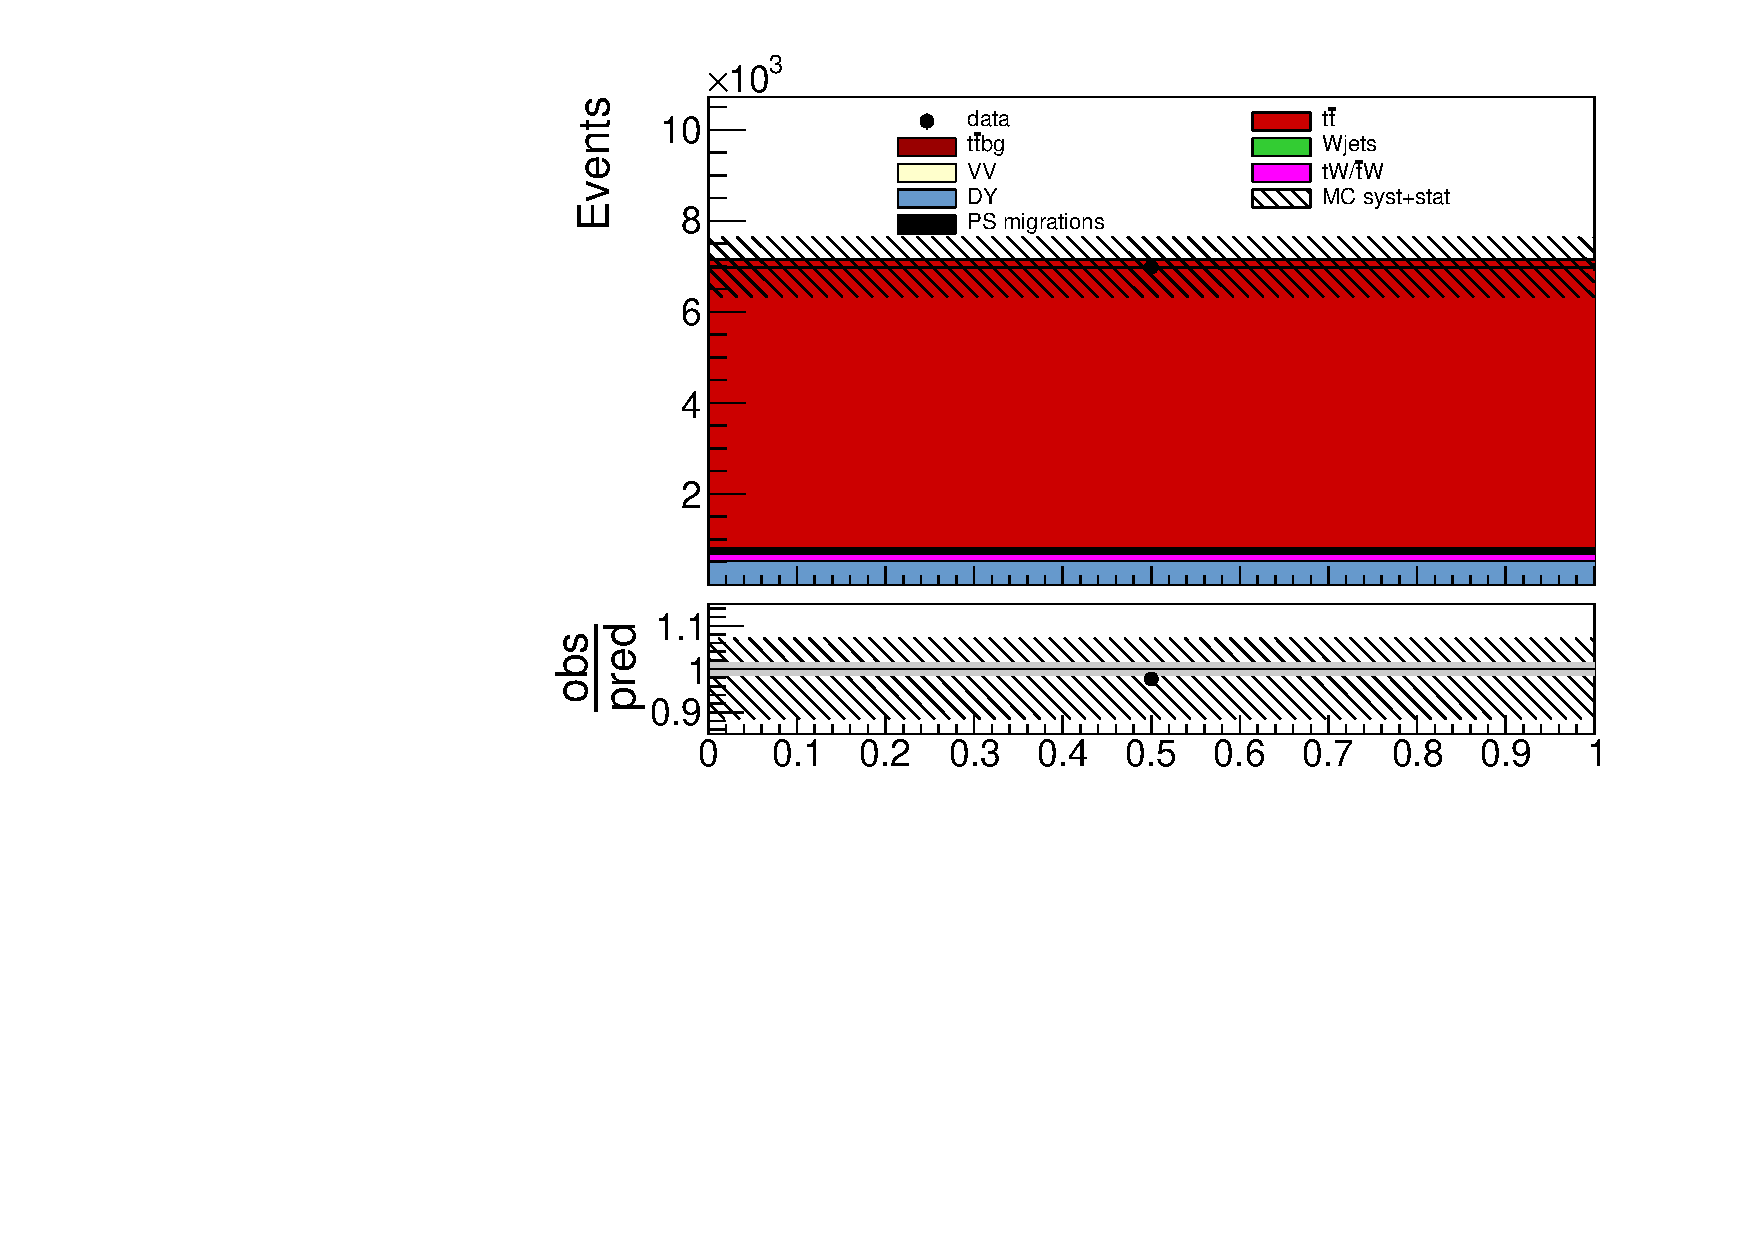
\includegraphics{CrossSection/Figures/ControlPlots/ee_sysnom/total_1_2_b-jets_step_8.pdf}}
    \resizebox{0.4 \textwidth}{!}{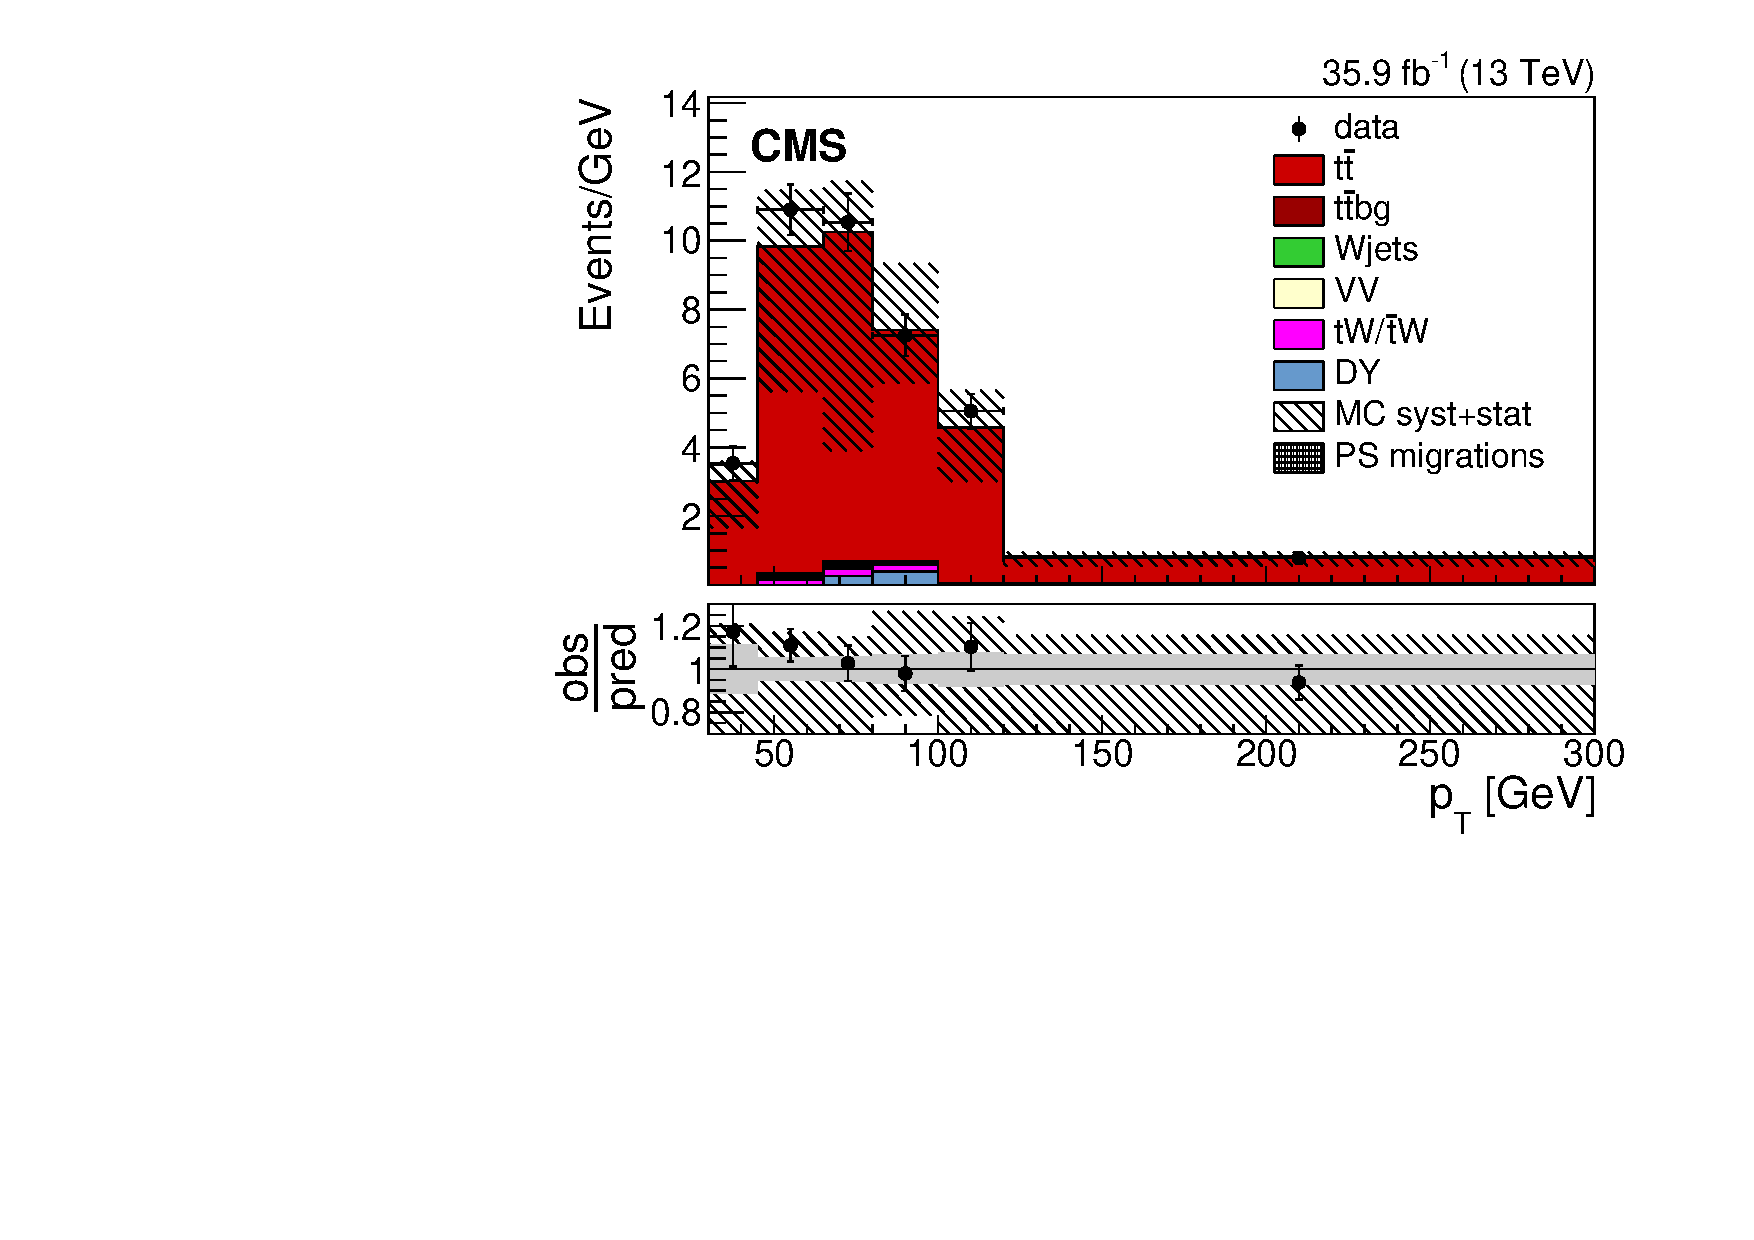
\includegraphics{CrossSection/Figures/ControlPlots/ee_sysnom/second_jet_pt_2_2_b-jets_step_8.pdf}}\\

    \resizebox{0.4 \textwidth}{!}{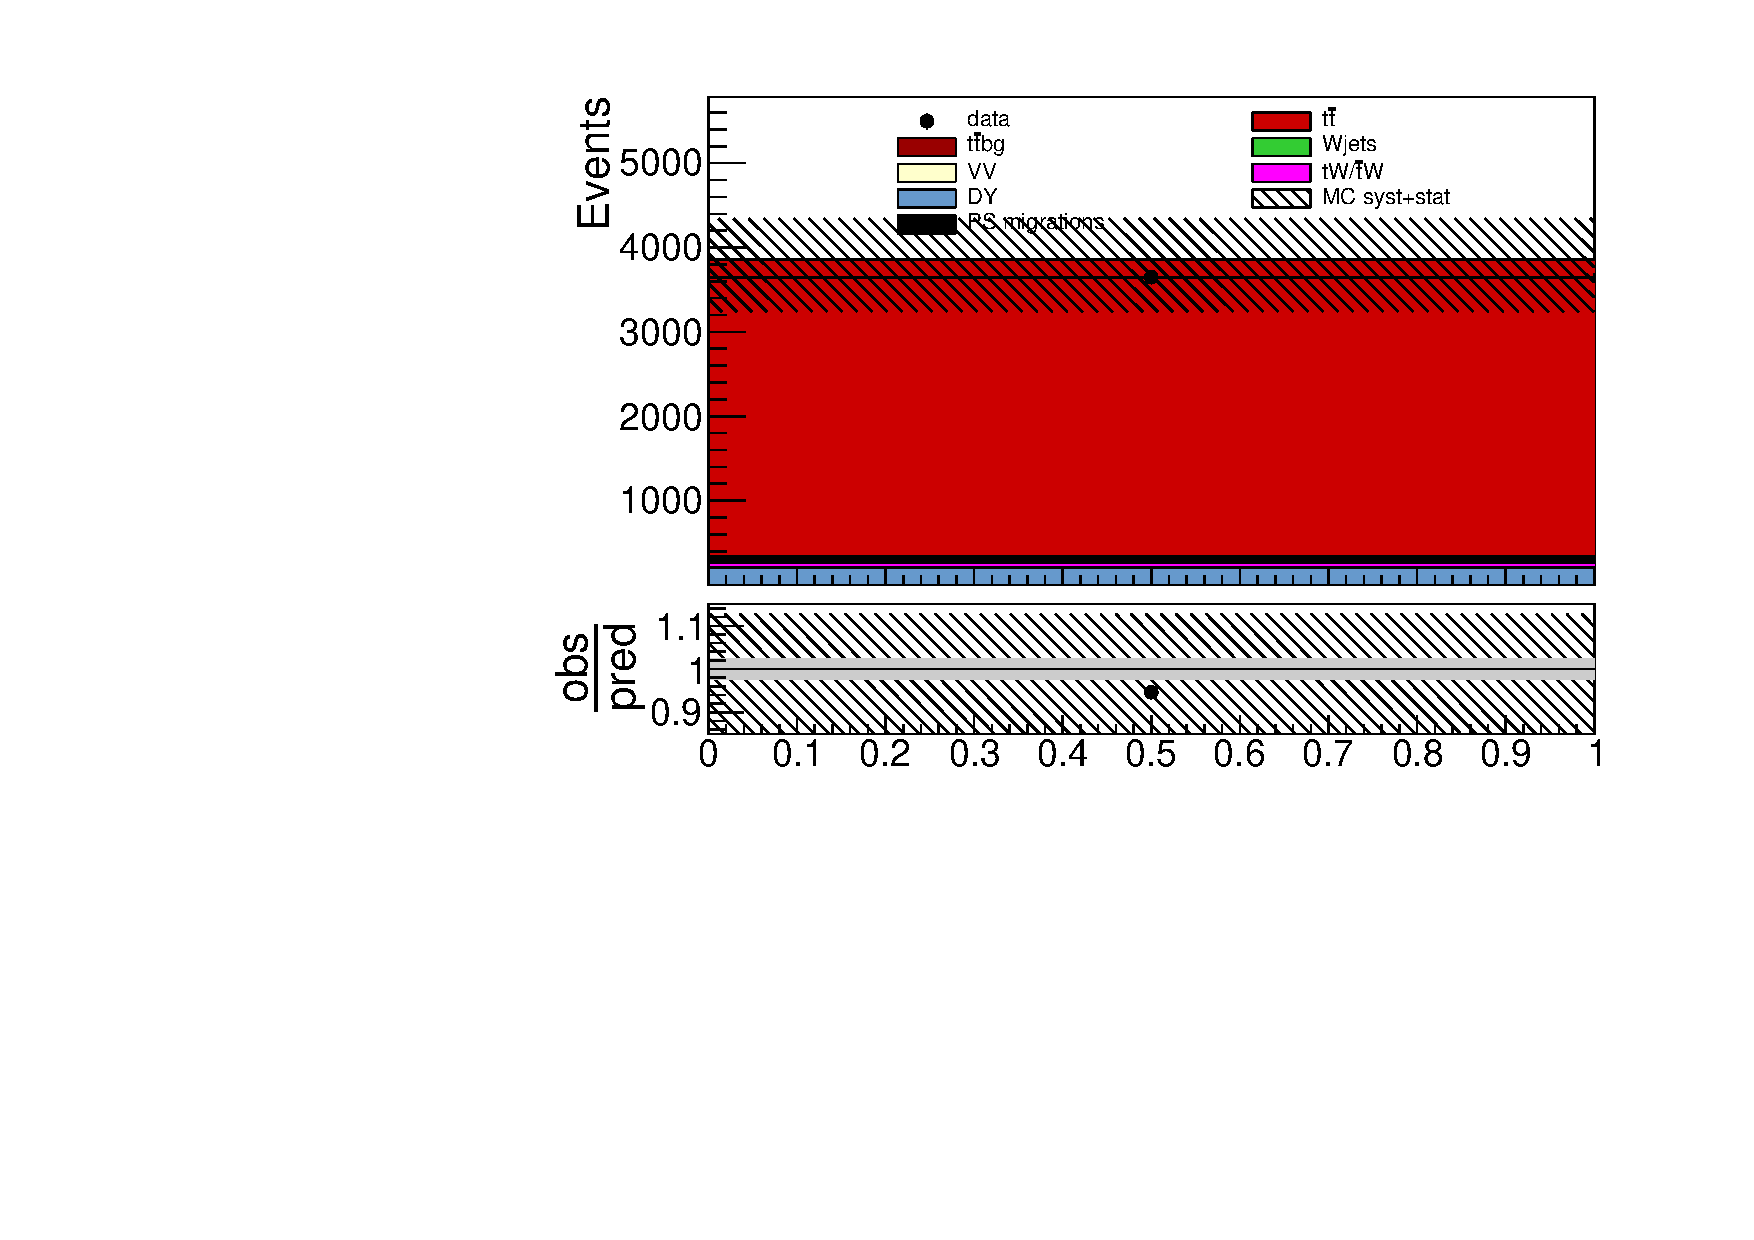
\includegraphics{CrossSection/Figures/ControlPlots/ee_sysnom/total_1_3_b-jets_step_8.pdf}}
    \resizebox{0.4 \textwidth}{!}{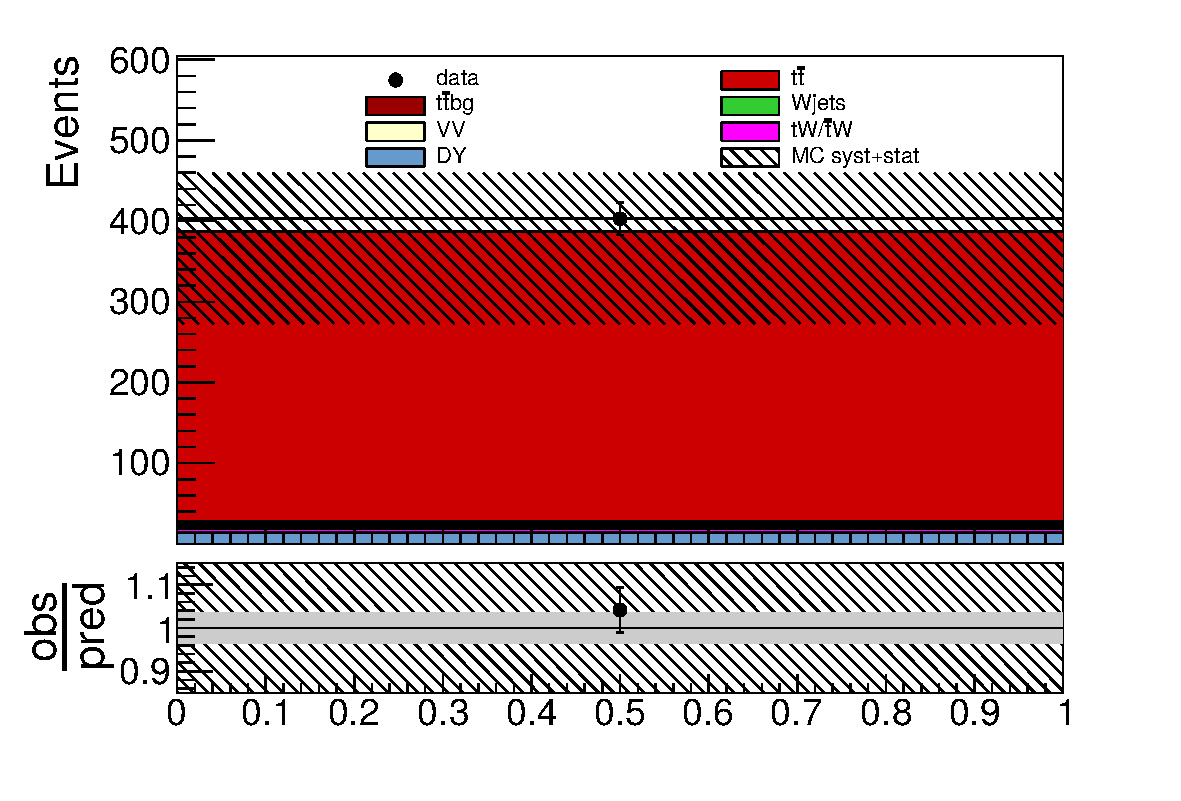
\includegraphics{CrossSection/Figures/ControlPlots/ee_sysnom/total_2_3_b-jets_step_8.pdf}} 
\caption{Template distributions for events in the \ee channel with one b-tagged jet (left column) or two b-tagged jets (right column). The distributions show the total event yield for zero (top), \pt of the jet with the lowest \pt  for one (second from top),
  two (second from bottom) or three or more (bottom) additional jets. 
  The hatched bands correspond to the total uncertainty on the predicted number of events, excluding luminosity and background
        normalization uncertainties.  The ratios of the event yields in data and the sum of the
  predicted yields are shown at the bottom of each figure. Here, the solid
  gray band represents the contribution of the statistical uncertainty.  
       \label{fig:xsec_ee_inputdistr}}
  \end{center}
\end{figure}


    
\section{Definition of the likelihood}
\label{sec:xsec_stat}

A binned likelihood fit is used to extract the \ttbar cross section using the event categorization described above. 
The number of expected events for signal and background is fitted to the number of measured events. 
The likelihood function used for the fit is based on poisson statistics:

\begin{eqnarray}
   \mathcal{L}  &=& \prod_{i} \frac{\exp{(\mu_i)} \mu_i^{n_i}}{n_i !}  + \prod_{l} \pi(\omega_l) + \prod_{m} \pi(\lambda_m) \\
 \mathrm{where} \; \; \; \; \; \mu_i &=& s_i(\sttvis,\vec{\lambda}) + \sum_{l} b_{l,i}(\omega_l,\vec{\lambda}).
\label{eq:xsec_chisqfunct}
\end{eqnarray}

Here the index $i$ represents a single bin, while $n_i$ is the number of measured events in data. The symbol $\mu_i$ represents the number
of expected events in simulation. The terms $\omega_l$ and $\lambda_m$
denote the nuisance parameters, with the $\pi$ standing for the penalty term related to the assumption of a Gaussian distribution for the nuisance parameter.
The second equation breaks down the expected number of events $\mu_i$ per bin $i$ into the number of signal events $s_i$, depending on the \ttbar cross section in the visible phase space $\sttvis$ and all relevant nuisance parameters $\vec{\lambda}$, and the number of
background events  $b_{l,i}$ for each background process $l$. The backgrounds also depend on the nuisance parameters and the normalization of the respective background process $\omega_l$.

The number of \ttbar events depends on the \ttbar production cross section, which allows to extract the latter from a fit of the former. Systematic uncertainties are included with nuisance parameters.
The normalization of the background processes is also included as a nuisance parameter separately for each of the background processes.

The nuisance parameters are fitted as well, but the allowed parameter space of each nuisance parameter is typically restricted according
to a priori assumptions based on external measurements. These assumptions are usually expressed as probability distributions also denoted as priors.
In case these probability distributions are not flat a so-called penalty term is introduced to the fit to express the improbability of finding such a value for this specific systematic uncertainty.

A unit normal distribution is chosen as probability density function for nuisance parameters with Gaussian priors. Other nuisance parameters have a uniform prior and do not contribute any penalty terms. 
Since a uniform probability distribution has either a constant value or a value of zero, no special term for the nuisance parameter is preferred (unless it is forbidden), consequently no penalty term is needed. 

As described above, the number of expected events for a background process also depends on the nuisance parameters. Especially nuisance parameters related to experimental systematic uncertainties affect the signal as well as the background processes. For example, the uncertainty on the muon reconstruction efficiency affects all events containing a muon (background as well as signal), while an uncertainty related to theory uncertainties usually only applies to the relevant process. The details can be found in Chapter~\ref{sec:syst_uncert}.

The number of background events can then be decomposed into:

\begin{equation}
b_{l,i}(\omega_l,\vec{\lambda}) = b_{l,i}^{MC}(\vec{\lambda}) \cdot (1 + \omega_l).
\label{eq:nbli}
\end{equation}

Here, $b_{l,i}^{MC}$ denotes the expected number of events from the simulation of the respective background process and $\omega_l$ denotes the normalization. The number of background events in simulation depends on the nuisance parameters $\vec{\lambda}$. The uncertainty on the normalization of a specific process is propagated
by variation of the respective $\omega_l$.

Following the description in Section~\ref{sec:xsec_templates},  the number of signal events is further divided according to the number of b-tagged jets.
The number of events in the categories for events with zero or more than two b-tagged jets $s_{0,b}$, for events with exactly one $s_{1,b}$ and for events with exactly two b-tagged jets $s_{2,b}$ are expressed as follows:

\begin{eqnarray}
s_{0,b}  &=& \lumi \cdot \sttvis\cdot \epsilon_{e\mu} \cdot (1-2\epsilon_b(1-C_b\epsilon_b)-C_b\epsilon_b^2) \\
s_{1,b}  &=& \lumi \cdot \sttvis \cdot \epsilon_{ll} \cdot 2 \epsilon_b(1-C_b\epsilon_b) \\
s_{2,b}  &=& \lumi \cdot \sttvis \cdot \epsilon_{ll} \cdot   \epsilon_b^2 C_b.
\label{eq:xsec_nb}
\end{eqnarray}
Only events in the \emu channel contribute to category $s_{0,b}$.
Here, $\lumi$ denotes the integrated luminosity, $\sttvis$ the visible \ttbar cross section and $\epsilon_{ll}$ the efficiency of the dilepton selection.
The b-tagging efficiency $\epsilon_b$ is the probability to reconstruct a b-tagged jet in a \ttbar event. It includes the efficiency of the b-tagging algorithm, the geometrical acceptance of the kinematic cuts on the b-tagged jet ($\pt > 30\; \GeV, |\eta|<2.4$) and the probability of a light jet to be b-tagged. In general, the contribution of the geometrical acceptance and the mis-tag rate is comparably low (see Section~\ref{sec:SimReco_BjetReco} for the mistag rate).
It is assumed that the two b-tagged jets can be identified independently of each other. Remaining correlations between the b-tagging efficiencies for both jets are described by the parameter $C_b$. These correlations can also be expressed in terms of the events measured in the separate categories: $C_b=4s_{ll}s_{2,b}/(s_{1,b}+2s_{2,b})^2$ where $s_{ll}$ is the total number of selected \ttbar events. 

The values for $\epsilon_{ll}$ and $s_{i}$ are obtained from simulation and depend on the nuisance parameters $\vec{\lambda}$. Any constraint of $\epsilon_{ll}$ and $s_{i}$ also constrains the related nuisance parameters $\lambda$.

The visible cross section $\sttvis$ corresponds to the cross section in the fiducial phase space as defined in Section~\ref{sec:xsec_sel}. The requirement to select one b-tagged jet in the same-flavor channels is absorbed into $\epsilon_{\mathrm{ee}}$ or $\epsilon_{\mu\mu}$ respectively.
In the fiducial phase space all systematic uncertainties and the related nuisance parameters can be constrained.

The dependence of the template distributions on the nuisance parameters is modeled with a second order polynomial which is constructed using the nominal and the two systematically varied values of each nuisance parameter $\lambda_m=0, 1, -1$.
The variation of the respective template distributions in each bin depends on the value of $\lambda$, with $\lambda = \pm 1$ corresponding to a $ \pm 1 \cdot \sigma$ variation. If multiple template distributions are affected by one uncertainty or nuisance parameter, all of them are varied coherently.
The template distributions are then added up to the expected number of events in each bin, as shown in Equation~\ref{eq:xsec_chisqfunct}. The expected number of events consequently mirrors the dependence of the template distributions on the nuisance parameters.
Some nuisance parameters are based on a one-sided variation so only one systematically varied value exists. In these cases, the dependence of the template distributions on the nuisance parameters is modeled by a linear function.

The MINUIT~\cite{James:1975dr} algorithm is used to minimize the  $-2 \ln{(\mathcal{L})}$ term (see~\ref{eq:xsec_chisqfunct} ) as function of the free fit parameters $\stt$, $\vec{\omega}$
and $\vec{\lambda}$. 

The nuisance parameters are a priori assumed to be uncorrelated, but the simultaneous fit takes possible correlations into account. Nuisance parameters having a similar effect on the fitted observables will be correlated by the fit.
An example for this are the nuisance parameters for the uncertainties on the lepton efficiencies, as already discussed in Section~\ref{sec:xsec_templates}. Both lepton efficiencies affect the number of events and the overall selection efficiency in a similar way in the \emu channel, leading to a strong correlation between these two parameters.

The choice of event categories and the parametrization of the likelihood function allow constraining several relevant systematic uncertainties of the \ttbar cross section.
Uncertainties related to jets and especially b jets are expected to be constrained after the fit. As shown below (see Chapter~\ref{sec:syst_uncert}) this includes a wide array of different systematic uncertainties
from the uncertainty on the b jet identification to the uncertainty on the scale for final state radiation in the parton shower. The uncertainties on the lepton efficiencies are expected to be constrained as well, due to the separation into the three decay channels.
Uncertainties that change the normalization of all processes like the uncertainty on the trigger efficiency or the luminosity are not expected to be constrained by the fit.


\section{Extrapolation from the visible to the full phase space}
\label{sec:xsec_extraction}

The previous section referred to the visible cross section in the fiducial phase space. In order to extrapolate this result to the full phase space an acceptance correction 
is determined.
Similar to the cross section itself, some of the uncertainties need to be extrapolated.

The acceptance can be introduced by replacing the efficiency of the dilepton selection as follows:

\begin{equation}
\epsilon_{ll} = A_{ll} \epsilon_{ll}.
\label{eq:epsacc}
\end{equation}

Here $A_{ll}$ is the acceptance and $\epsilon_{ll}$ is the efficiency in the visible phase space, both depending on the nuisance parameters $\vec{\lambda}$.
Correspondingly, the visible cross section can be extrapolated to the full cross section by dividing it by the acceptance: $\sttbar = \sttvis / A_{ll}$, again both the visible cross section and the 
acceptance depend on the nuisance parameters.

The acceptance is defined by the kinematic selection requirements on the leptons. As detailed in Section~\ref{sec:xsec_sel} the two leptons are required to be part of the $t \rightarrow W b$ decay. They are further required to be within $|\eta|< 2.4$ with the 
leading lepton having $\pt > 25 \; \GeV$ and the trailing lepton $\pt > 20 \; \GeV$. The invariant mass of the dilepton system is required to be $\mll > 20 \; \GeV$. The acceptance is calculated as the ratio of the number of \ttbar events that fulfill these requirements to all \ttbar events.

The values for the nuisance parameters that are determined in the fit of the visible cross section are propagated to the acceptance, including the correlations between the nuisance parameters. 
Similarly, the constraints for most of the nuisance parameters are applied to the calculation of the uncertainty of the acceptance.
Some of the nuisance parameters that are constrained in the visual phase space are unconstrained in the extrapolation.
Since the acceptance is defined in the simulation, after the parton shower, but before the detector simulation, uncertainties on the 
matrix element and parton shower affect the acceptance.

The following uncertainties are extrapolated:
The uncertainty on the PDF, the top \pt uncertainty, the uncertainty on the matrix element scale and the uncertainties on the parton shower tune, the initial and final state radiation scales.

The extrapolation of an uncertainty takes the fitted value of each relevant nuisance parameter as central value. Then the change of acceptance for the explicit $\pm 1 \sigma$ variation is considered as the $\pm 1 \sigma$ variation on the acceptance. The additional uncertainties are then added to the uncertainty of the cross section, extrapolated to the full phase space, for each relevant nuisance parameter. The additional uncertainties are treated as uncorrelated and are added up in quadrature. This procedure can lead to asymmetric variations, even for originally symmetric variations in case the fitted value of the nuisance parameter is not the original central value.

Before discussing the results in Section~\ref{sec:results_main}, the next chapter gives a detailed description of the systematic uncertainties.

